%\documentclass[final,subfig,blackref,approvalform]{drexel-thesis} %final copy
%\documentclass[final,subfig,blackref]{drexel-thesis} %final copy
\documentclass[final,subfig,daring]{drexel-thesis} %colorful links copy
%\documentclass[daring,subfig,blackref,draftspace]{drexel-thesis} %for committee
%\documentclass[daring,subfig,blackref,draftwatermark,draftspace]{drexel-thesis} %draft copy

%swap margins so the wide one is down the binding edge when printing double sided
%only use this with twoside
%\let\tmp\oddsidemargin
%\let\oddsidemargin\evensidemargin
%\let\evensidemargin\tmp
%\reversemarginpar

% packages for CV formatting
\usepackage{marvosym}
\usepackage{url,parskip}   %other packages for formatting
\RequirePackage{color,graphicx}
%\usepackage[usenames,dvipsnames]{xcolor}
%\usepackage{fullpage} 
\usepackage{longtable}
\usepackage[super]{nth}

\usepackage{verbatim}
\usepackage{amsmath}
\usepackage{amssymb}
\usepackage{placeins}   % To allow pictures to flush after a section
\usepackage{setspace}
\usepackage{nth}

% Draft mode on the pictures
% \setkeys{gin}{draft}

% Fancy citation extensions
\usepackage[super,sort&compress,comma]{natbib}
%\bibliographystyle{yahapj}
\bibliographystyle{ieeetr}

% fncychap clobbers \appendix with a silly implementation that breaks
% hyperlinks to appendix chapters.  Work around this by ignoring their
% implementation completely.
\let\temporaryAppendix\appendix
\usepackage[Conny]{fncychap}  % Nicer style used for distribution
%\usepackage[]{fncychap}
\let\appendix\temporaryAppendix

\usepackage{deluxetable}
%\usepackage{aastex_hack}
\usepackage{tikz}
\usepackage{tkz-berge}
\usetikzlibrary{shapes}
%\usepackage[left]{showlabels}


\ChRuleWidth{1.5pt}
\ChTitleVar{\Large \sc \bf}
\ChNumVar{\Large \sc \bf}
\ChNameVar{\Large \sc \bf}

% Spacings between the chapter top and to the text
%-----------------------------------------------------------------------------
\newcommand{\chaptertopspacing}{10}
\newcommand{\chaptertotextspacing}{-10}
\newcommand{\chaptertopspacingSTAR}{10}
\newcommand{\chaptertotextspacingSTAR}{-10}

\iffinal{}{  % Library format requires numbered footnotes
\renewcommand{\thefootnote}{$\dagger$}	% Daggers for footnote markers style
}

% Convenience functions
% -----------------------------------------------------------------------------
\newcommand{\B}[1]{ {\bf #1} }      		% Bold text for matrices
\newcommand{\Z}{\mathcal{Z}}				% Partition function
\newcommand{\HAM}{\mathcal{H}}		% Hamiltonian
\newcommand{\qp}[0]{(\B{q},\B{p})}  % Cannonical variables (q,p) 
\newcommand{\pfrac}[2]{\frac{\partial #1}{\partial #2}} 	% partial 1 /partial 2 
%\newcommand{\fr}{2}{\frac{#1}{#2}}   % frac 1/2
\newcommand{\ket}[1]  {\left | \, #1 \right \rangle}			% bra-ket notation
\newcommand{\abs}[1]{\left\vert #1 \right\vert}		% vert bars for averages
\newcommand{\norm}[1]{\left\Vert #1 \right\Vert}	% taller vert bars for the norm
\newcommand{\evalat}[1]{\left. #1 \right \vert}	% ex. evaluating the int. at its limits
\newcommand{\set}[1]{\left\{ #1 \right\}}					% squigle brackets for sets
\newcommand{\avg}[1]{\left< #1 \right>}					% angle brackets for averages
\newcommand{\paren}[1]{\left( #1 \right)}					% grows parentheses to the correct size
\newcommand{\brackets}[1]{\left[ #1 \right]}			% grows square brackets
\newcommand{\braces}[1]{\left \{ #1 \right \}}
\newcommand{\piecewisebrace}[1]{\left \{ #1 \right .} % Useful for piecewise functions

\newcommand{\ie}{i.e.\ }
\newcommand{\eg}{e.g.\ }
\newcommand{\cf}{c.f.\ }
\newcommand{\chem}[1]{\ensuremath{\mathrm{#1}}} % Chemical formula

\DeclareMathOperator*{\minor}{minor\,}
\DeclareMathOperator*{\sgn}{\mathbf{sgn}\,}
\DeclareMathOperator*{\rootof}{RootOf\,}


\newcommand{\figurewidthSINGLE}{0.8\textwidth}
\newcommand{\figurewidthDOUBLE}{0.45\textwidth}
\newcommand{\figurewidthTRIPLE}{0.35\textwidth}

\newcommand{\CHI}[2]{\chi_{#1 #2}} % Cluster Counting function

% ----------------------------------------------------------------------------

\newcommand{\civ}{\ion{C}{4}}
\newcommand{\athree}{$\alpha_{\rm 3D}$}
\newcommand{\aone}{$\alpha_{\rm 1D}$}
\newcommand{\atwo}{$\alpha_{\rm 2D}$}
\newcommand{\luvaox}{$L_{\rm }$--$\alpha_{\rm ox}$}
\newcommand{\lbol}{$L_{\rm bol}$}
\newcommand{\luv}{$L_{\rm uv}$}
\newcommand{\lx}{$L_{\rm x}$}
\newcommand{\llam}{$L_{\lambda}$}
\newcommand{\ltwofive}{$L_{\rm 2500\,\AA}$}
\newcommand{\lfiveone}{$L_{\rm 5100\,\AA}$}
\newcommand{\bctwofive}{BC$_{\rm 2500\,\AA}$}
\newcommand{\bcfiveone}{BC$_{\rm 5100\,\AA}$}
\newcommand{\onemum}{1\,$\mu$m}
\newcommand{\tenmum}{10\,$\mu$m}
\newcommand{\thirtymum}{30\,$\mu$m}
\newcommand{\twokev}{2\,keV}
\newcommand{\tenkev}{10\,keV}
\newcommand{\hundredev}{0.1\,keV}
\newcommand{\twohundredev}{0.2\,keV}
\newcommand{\ebv}{{\rm E(B-V)}}
\newcommand{\dal}{\Delta(\alpha_{\lambda})}
\newcommand{\dgi}{\Delta(g-i)}
\newcommand{\dug}{\Delta(u-g)}
\newcommand{\diz}{\Delta(i-z)}
\newcommand{\mrel}{\Delta m}
\newcommand{\mbh}{M_{\rm BH}}
\newcommand{\lmbh}{\log{(M_{\rm BH})}}
%\newcommand{\lf}{L_{\rm frac}}
\newcommand{\lf}{L/L_{\rm Edd}}

% ----------------------------------------------------------------------------
% Override the color of links
%\newif\if@colorref
\hypersetup{colorlinks}
%\if@colorref
  \hypersetup{linkcolor=blue}
  \hypersetup{anchorcolor=black}
  \hypersetup{citecolor=blue}
  \hypersetup{filecolor=black}
  \hypersetup{menucolor=black}
  \hypersetup{runcolor=black}
  \hypersetup{urlcolor=blue}
\fi

% Partition block notation
% -----------------------------------------------------------------------------
\newcommand*\pblock[3]{
	\tikz[baseline=(char.base)]{
		\node[ellipse,draw,inner sep=2pt] (char) {$#1$};
	} ^{#2}_{#3}
}

\newcommand{\Go}{\text{G}\bar{\text{o}}}
\newcommand{\GO}{\textbf{G}}
\newcommand{\CHIX}{\mathbf{X}}
\newcommand{\KP}{k_+}
\newcommand{\KM}{k_-}
\newcommand{\KPMAX}{k_+^*}

% -----------------------------------------------------------------------------
% Add the CC logo to the copyright page and spruce it up a bit
\renewcommand\copyrighttextCCBYSA{
\\[2 em]
\begin{quote}
\begin{center}

\includegraphics[width=.3\textwidth]{pictures/cc_logo.pdf} \\[2 em]
\end{center} 
    This work is licensed under the terms of the Creative Commons
    Attribution-ShareAlike 4.0 International license.  The license is
    available at \\
    \url{http://creativecommons.org/licenses/by-sa/4.0/}.
\end{quote}
}

% -----------------------------------------------------------------------------
% Environment for temporarily removing the page footer
\newcommand{\suppressfooter}
{%
\fancyfoot[RE,LO,LE,RO]{}
\renewcommand{\footrulewidth}{0.0pt}
}%

\newcommand{\restorefooter}
{%
\fancyfoot[RE,LO]{\scshape\leftmark}
\fancyfoot[LE,RO]{\scshape\rightmark}
\renewcommand{\footrulewidth}{.4pt}
}%

\newcommand{\rightfooter}
{%
%\fancyfoot[RE,LO]{\scshape\leftmark}
\fancyfoot[LE,RO]{\scshape\rightmark}
\renewcommand{\footrulewidth}{.4pt}
}%

% -----------------------------------------------------------------------------
% Simple command for inline figures (does not count towards a normal figure)

\newcommand{\inlinespacing}{1em}
\newcommand{\inlineframebox}[2]{
\vspace{1em}
\newline
\fbox{
\begin{minipage}[]{.95 \linewidth}
\begin{center}
#1 \\
#2
\end{center}
\end{minipage}
}
\vspace{1em}
\newline
}

\newcommand{\inlinembox}[2]{
\vspace{1em}
\newline
\begin{minipage}[]{.95 \linewidth}
\begin{center}
#1 \\
#2
\end{center}
\end{minipage}
\vspace{1em}
\newline
}


% -----------------------------------------------------------------------------
% Custom styling for quote boxes, use \epigraph

\definecolor{quotationcolour}{HTML}{F0F0F0}
\definecolor{quotationmarkcolour}{HTML}{1F3F81}

\newcommand{\epiline}{\hrule \vskip -.2em \hrule}
% Massively humongous opening quotation mark.
\newcommand{\hugequote}[1]{%
  \fontsize{42}{48}\selectfont \color{quotationmarkcolour} \textbf{#1}
  \vskip -.5em
}

\newcommand{\epigraph}[2]{%
  \smallskip
 \begin{center}
%  \hspace{1em}
  \colorbox{quotationcolour}{%
    \parbox{.8\textwidth}{%
    \epiline \vskip 1em 
    #1
    \begin{flushright}\textsc{#2}\end{flushright}
    \epiline
    }
  }
  \end{center}
  \medskip
}

\newcommand{\epigraphshort}[1]{%
  \smallskip
 \begin{center}
%  \hspace{1em}
  \colorbox{quotationcolour}{%
    \parbox{.8\textwidth}{%
    \epiline \vskip 1em 
     \begin{center}
    #1
    \end{center}

    \epiline
    }
  }
  \end{center}
  \medskip
}

% -----------------------------------------------------------------------------
% custom DRAFT MARK

\usepackage[]{datetime} 
\usepackage[allpages]{draftmark}

\iffinal{}{
\draftmarksetup{
  angle=0,scale=.34,
  color=red!45!blue!25,xcoord=117,ycoord=-129,
  mark={  \raggedright \mmddyyyydate (DRAFT)\\ \today} }
}

% -----------------------------------------------------------------------------
% Customize fncychap settings
\iffinal{}{
	\ChRuleWidth{1.5pt}
	\ChTitleLowerCase
	\ChTitleVar{\Huge \sc}
	}

% -----------------------------------------------------------------------------
% tighten the fncychap spacings, TeX code taken from
% http://tex.stackexchange.com/questions/13357/fncychap-package-reduce-vertical-gap-space-between-header-and-chapter-heading

\makeatletter
\renewcommand*{\@makechapterhead}[1]{%
  \iffinal{\setstretch{\@ssp}}{}
  
  \vspace*{\chaptertopspacing\p@}%
  {\parindent \z@ \raggedright \normalfont
    \ifnum \c@secnumdepth >\m@ne
      \if@mainmatter%%%%% Fix for frontmatter, mainmatter, and backmatter 040920
        \DOCH
      \fi
    \fi
    \interlinepenalty\@M
    \if@mainmatter%%%%% Fix for frontmatter, mainmatter, and backmatter 060424
      \DOTI{#1}%
    \else%
      \DOTIS{#1}%
    \fi
    \vspace*{\chaptertotextspacing\p@}
  }
  \iffinal{\setstretch{\@dsp}}{}  
}


 \renewcommand*{\@makeschapterhead}[1]{%
  \vspace*{\chaptertopspacingSTAR\p@}%
  {\parindent \z@ \centering%\raggedright
    \normalfont
    \interlinepenalty\@M
    \DOTIS{#1}
    \vskip \chaptertotextspacingSTAR\p@
  }}
 
\makeatother


% -----------------------------------------------------------------------------
% redefine abstract from drexel-thesis since the spacing is now wrong
\makeatletter
\renewenvironment{abstract}{%
  \listed@schapter{\abstractname}%
  \blanklines{-0}%
    \begin{center}
      \setstretch{\@ssp}%
      \@DUT@title\\
      \@DUT@author\\
      \ifdaring{%
        \ifnum\c@@DUT@advisors=\@ne%
        Advisor:
        \else%
        Advisors:
        \fi}{}
      \@DUT@advisor\\
    \end{center}
  \blanklines{4}%
  \setstretch{\@dsp}%
  \@nobreaktrue
  \@afterindentfalse
  \@afterheading
}{%
  \par\setstretch{\@ssp}%
}
\makeatother


\includeonly{
	tex/preamble,           %Dedications, acknowledgments, TOC, and abstract
	tex/Introduction,       %CHAPTER: Introduction
	tex/Data,               %CHAPTER: Experimental Results
	tex/LM,               %CHAPTER: Light Management
	tex/ED,               %CHAPTER: Electronic Density Distribution
	tex/RM,                 %CHAPTER: Rate Management
	tex/LT,                 %CHAPTER: Laser Threshold Calculation
	tex/Conclusion,         %CHAPTER: Conclusion
	tex/appendix,           %APPENDIX
	tex/CV,                 %CV
}

\author{Zhihuan Wang}
\title{Dimensional Dependence of Light Interaction with Nanowires}
\DUTmonth{June}
\DUTyear{2017}
\degree{Doctor of Philosophy}
\advisor{Dr. Bahram Nabet}
\copyrighttext{\copyrighttextCCBYSA}

\tikzstyle{vertex}=[circle,fill=black!25,minimum size=10pt,inner sep=2pt]
\tikzstyle{Nvertex}=[circle,fill=white!25,minimum size=10pt,inner sep=2pt]
\tikzstyle{LabelStyle}=[fill=white,sloped]

\tikzstyle{big_vertex}=[circle,fill=red!15,minimum size=50pt,inner sep=2pt,draw=black!50]
\tikzstyle{med_vertex}=[circle,fill=red!10,minimum size=35pt,inner sep=2pt,draw=black!50]

\tikzstyle{macrostate_vertex}=[inner sep=3pt,draw=black!70]


\newcommand{\vertexshiftamount}{2.5}
\newcommand{\tikzpicscale}{1.5}

\newcommand{\TIKZenergylevel}{

  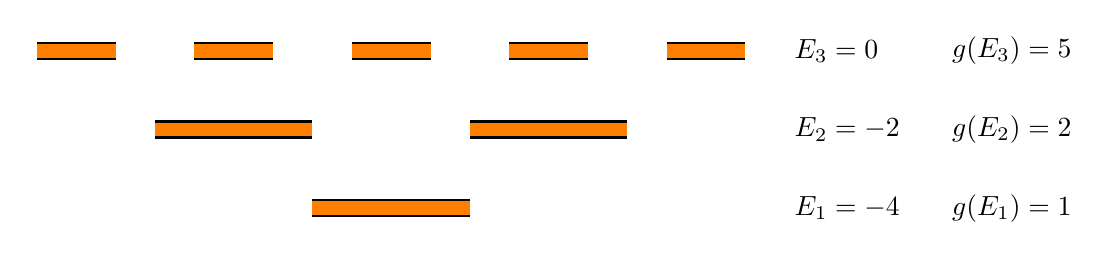
\begin{tikzpicture}
    \tikzset{level/.style   = {thick,
        double          = orange,
        double distance = 5pt}}
    
    \def\Espace{9};
    \def\Gspace{11};
    
    % Draw the energy levels.
    \draw[level] (3,0)  -- (5,0) node[right]{};
    \draw[] (\Espace,0) node[right] {$E_1=-4$};
    \draw[] (\Gspace,0) node[right] {$g(E_1)=1$};
    
    \draw[level] (1,1) -- (3,1) node[right] {};
    \draw[level] (5,1) -- (7,1) node[right] {};
    \draw[] (\Espace,1) node[right] {$E_2=-2$};
    \draw[] (\Gspace,1) node[right] {$g(E_2)=2$};
    
    \def\v{.5}; 
    \draw[level] (-1+\v,2) -- (0+\v,2) node[right] {};
    \draw[level] (1+\v,2) -- (2+\v,2) node[right] {};
    \draw[level] (3+\v,2) -- (4+\v,2) node[right] {};
    \draw[level] (5+\v,2) -- (6+\v,2) node[right] {};
    \draw[level] (7+\v,2) -- (8+\v,2) node[right] {};
    \draw[] (\Espace,2) node[right] {$E_3=0$};
    \draw[] (\Gspace,2) node[right] {$g(E_3)=5$};
  \end{tikzpicture}
}

\newcommand{\TIKZenergylevelSHORT}{

  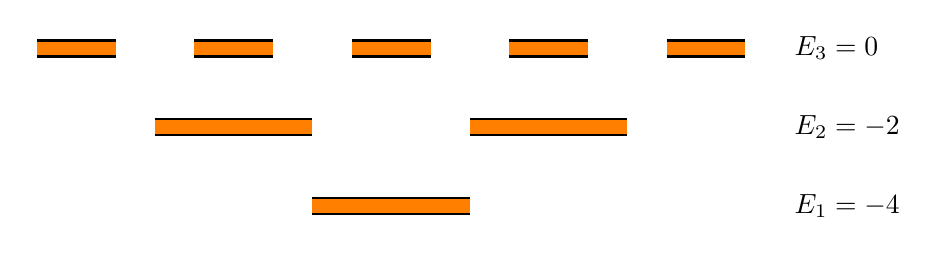
\begin{tikzpicture}
    \tikzset{level/.style   = {thick,
        double          = orange,
        double distance = 5pt,
        scale = 1.
        }}
    
    \def\Espace{9};
    \def\Gspace{11};
    
    % Draw the energy levels.
    \draw[level] (3,0)  -- (5,0) node[right]{};
    \draw[] (\Espace,0) node[right] {$E_1=-4$};
   
    \draw[level] (1,1) -- (3,1) node[right] {};
    \draw[level] (5,1) -- (7,1) node[right] {};
    \draw[] (\Espace,1) node[right] {$E_2=-2$};
    
    \def\v{.5}; 
    \draw[level] (-1+\v,2) -- (0+\v,2) node[right] {};
    \draw[level] (1+\v,2) -- (2+\v,2) node[right] {};
    \draw[level] (3+\v,2) -- (4+\v,2) node[right] {};
    \draw[level] (5+\v,2) -- (6+\v,2) node[right] {};
    \draw[level] (7+\v,2) -- (8+\v,2) node[right] {};
    \draw[] (\Espace,2) node[right] {$E_3=0$};
  \end{tikzpicture}
}


\newcommand{\TIKZgraphABC}{
  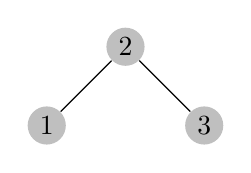
\begin{tikzpicture}[shorten >=1pt,->]
    \tikzstyle{vertex}=[circle,fill=black!25,minimum size=12pt,inner sep=2pt]
    \node[vertex] (G_1) at (-1,-1) {1};
    \node[vertex] (G_2) at (0,0)   {2};
    \node[vertex] (G_3) at (1,-1)  {3};
    \draw (G_1) -- (G_2) -- (G_3) -- cycle;
  \end{tikzpicture}
}

\newcommand{\TIKZgraphAB}{
  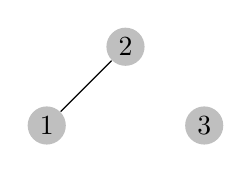
\begin{tikzpicture}[shorten >=1pt,->]
    \tikzstyle{vertex}=[circle,fill=black!25,minimum size=12pt,inner sep=2pt]
    \node[vertex] (G_1) at (-1,-1) {1};
    \node[vertex] (G_2) at (0,0)   {2};
    \node[vertex] (G_3) at (1,-1)  {3};
    \draw (G_1) -- (G_2) -- cycle;
  \end{tikzpicture}
}

\newcommand{\TIKZgraphBC}{
  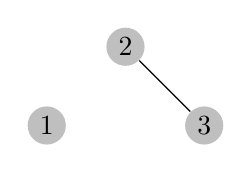
\begin{tikzpicture}[shorten >=1pt,->]
    \tikzstyle{vertex}=[circle,fill=black!25,minimum size=12pt,inner sep=2pt]
    \node[vertex] (G_1) at (-1,-1) {1};
    \node[vertex] (G_2) at (0,0)   {2};
    \node[vertex] (G_3) at (1,-1)  {3};
    \draw (G_2) -- (G_3) -- cycle;
  \end{tikzpicture}
}

\newcommand{\TIKZgraphC}{
  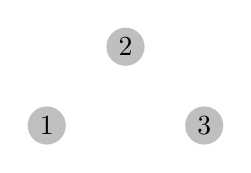
\begin{tikzpicture}[shorten >=1pt,->]
    \tikzstyle{vertex}=[circle,fill=black!25,minimum size=12pt,inner sep=2pt]
    \node[vertex] (G_1) at (-1,-1) {1};
    \node[vertex] (G_2) at (0,0)   {2};
    \node[vertex] (G_3) at (1,-1)  {3};
  \end{tikzpicture}
}


\newcommand{\TIKZgraphoneline}{
  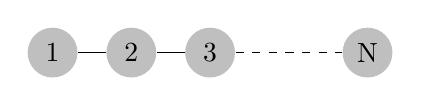
\begin{tikzpicture}[shorten >=1pt,->]
    \tikzstyle{vertex}=[circle,fill=black!25,minimum size=18pt,inner sep=2pt]
    \node[vertex] (G1) at (0,0)   {1};
    \node[vertex] (G2) at (1,0)   {2};
    \node[vertex] (G3) at (2,0)   {3};
    \node[vertex] (GN) at (4,0)   {N};
    \draw (G1) -- (G2) -- (G3) -- cycle;
    \draw[dashed] (G3) -- (GN) -- cycle;
  \end{tikzpicture}
}


\newcommand{\TIKZgraphtwoline}{
  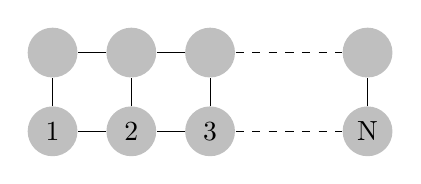
\begin{tikzpicture}[shorten >=1pt,->]
    \tikzstyle{vertex}=[circle,fill=black!25,minimum size=18pt,inner sep=2pt]
    \node[vertex] (G1) at (0,0)   {1};
    \node[vertex] (G2) at (1,0)   {2};
    \node[vertex] (G3) at (2,0)   {3};
    \node[vertex] (GN) at (4,0)   {N};
    \draw (G1) -- (G2) -- (G3) -- cycle;
    \draw[dashed] (G3) -- (GN) -- cycle;

    \node[vertex] (GN1) at (0,1)   {};
    \node[vertex] (GN2) at (1,1)   {};
    \node[vertex] (GN3) at (2,1)   {};
    \node[vertex] (G2N) at (4,1)   {};
    
    \draw (GN1) -- (GN2) -- (GN3) -- cycle;
    \draw (GN) -- (G2N) -- cycle;
    \draw (G1) -- (GN1) -- cycle;
    \draw (G2) -- (GN2) -- cycle;
    \draw (G3) -- (GN3) -- cycle;
    \draw (GN) -- (G2N) -- cycle;

    \draw[dashed] (GN3) -- (G2N) -- cycle;


  \end{tikzpicture}
}



\newcommand{\TIKZtwoladdera}{
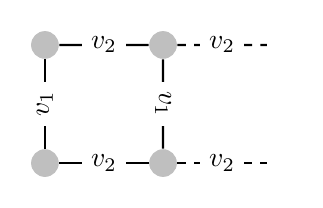
\begin{tikzpicture}[scale=\tikzpicscale]
    \node[vertex] (G1) at (0,0)   {};
    \node[vertex] (G2) at (1,0)   {};
    \node[vertex] (GA) at (0,1)   {};
    \node[vertex] (GB) at (1,1)   {};
	 \Edge[label=$v_2$](G1)(G2)
	 \Edge[label=$v_2$](GA)(GB)
	 \Edge[label=$v_1$](G1)(GA)
	 \Edge[label=$v_1$](G2)(GB)
    \node[Nvertex] (G3) at (2,0)   {};
    \node[Nvertex] (GC) at (2,1)   {};
	 \tikzstyle{EdgeStyle}=[dashed]
	 \Edge[label=$v_2$](G2)(G3)
	 \Edge[label=$v_2$](GB)(GC)
\end{tikzpicture}
}

\newcommand{\TIKZtwoladderb}{
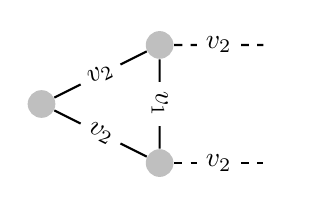
\begin{tikzpicture}[scale=\tikzpicscale]
    \node[vertex] (G2) at (1,0)   {};
    \node[vertex] (GB) at (1,1)   {};
    \node[vertex] (G1A) at (0,.5)   {};
	 \Edge[label=$v_2$](G1A)(G2)
	 \Edge[label=$v_2$](G1A)(GB)
	 \Edge[label=$v_1$](G2)(GB)
    \node[Nvertex] (G3) at (2,0)   {};
    \node[Nvertex] (GC) at (2,1)   {};
	 \tikzstyle{EdgeStyle}=[dashed]
	 \Edge[label=$v_2$](G2)(G3)
	 \Edge[label=$v_2$](GB)(GC)
\end{tikzpicture}
}

\newcommand{\TIKZtwoladderc}{
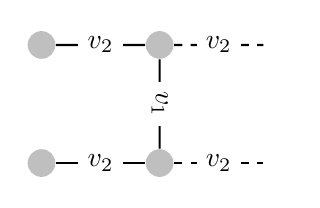
\begin{tikzpicture}[scale=\tikzpicscale]
    \node[vertex] (G1) at (0,0)   {};
    \node[vertex] (G2) at (1,0)   {};
    \node[vertex] (GA) at (0,1)   {};
    \node[vertex] (GB) at (1,1)   {};
	 \Edge[label=$v_2$](G1)(G2)
	 \Edge[label=$v_2$](GA)(GB)
	 %\Edge[label=$v_1$](G1)(GA)
	 \Edge[label=$v_1$](G2)(GB)
    \node[Nvertex] (G3) at (2,0)   {};
    \node[Nvertex] (GC) at (2,1)   {};
	 \tikzstyle{EdgeStyle}=[dashed]
	 \Edge[label=$v_2$](G2)(G3)
	 \Edge[label=$v_2$](GB)(GC)
\end{tikzpicture}
}

\newcommand{\TIKZtwoladderd}{
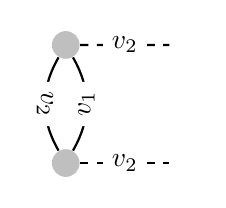
\begin{tikzpicture}[scale=\tikzpicscale]
    \node[vertex] (G2) at (1,0)   {};
    \node[vertex] (GB) at (1,1)   {};
	 %\Edge[label=$v_1$](G1)(GA)
	\tikzstyle{EdgeStyle}=[bend left]
	\Edge[label=$v_2$](G2)(GB)
  	\tikzstyle{EdgeStyle}=[bend right]
	\Edge[label=$v_1$](G2)(GB)
    \node[Nvertex] (G3) at (2,0)   {};
    \node[Nvertex] (GC) at (2,1)   {};
	 \tikzstyle{EdgeStyle}=[dashed]
	 \Edge[label=$v_2$](G2)(G3)
	 \Edge[label=$v_2$](GB)(GC)
\end{tikzpicture}
}

\newcommand{\TIKZtwoladdere}{
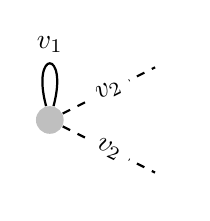
\begin{tikzpicture}[scale=\tikzpicscale]
    \node[vertex] (G2B) at (1,.5)   {};
	 %\Edge[label=$v_1$](G1)(GA)
	\tikzstyle{EdgeStyle}=[loop above]
	\Edge[label=$v_1$](G2B)(G2B)
   \node[Nvertex] (G3) at (2,0)   {};
   \node[Nvertex] (GC) at (2,1)   {};
	\tikzstyle{EdgeStyle}=[dashed]
	\Edge[label=$v_2$](G2B)(G3)
	\Edge[label=$v_2$](G2B)(GC)
\end{tikzpicture}
}

\newcommand{\TIKZtwoladderf}{
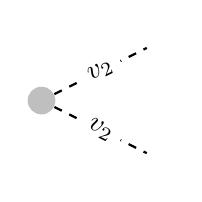
\begin{tikzpicture}[scale=\tikzpicscale]
    \node[vertex] (G2B) at (1,.5)   {};
   \node[Nvertex] (G3) at (2,0)   {};
   \node[Nvertex] (GC) at (2,1)   {};
	\tikzstyle{EdgeStyle}=[dashed]
	\Edge[label=$v_2$](G2B)(G3)
	\Edge[label=$v_2$](G2B)(GC)
\end{tikzpicture}
}

\newcommand{\TIKZthreeladderA}{
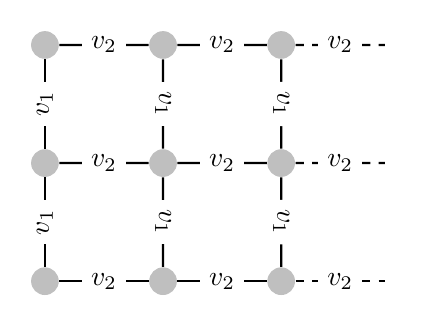
\begin{tikzpicture}[scale=\tikzpicscale]
    \node[vertex] (00) at (0,0)   {};
    \node[vertex] (10) at (1,0)   {};
	 \node[vertex] (20) at (2,0)   {};
    \node[vertex] (01) at (0,1)   {};
    \node[vertex] (11) at (1,1)   {};
    \node[vertex] (21) at (2,1)   {};
    \node[vertex] (02) at (0,2)   {};
    \node[vertex] (12) at (1,2)   {};
    \node[vertex] (22) at (2,2)   {};
	 \Edge[label=$v_2$](00)(10)
	 \Edge[label=$v_2$](10)(20)
	 \Edge[label=$v_2$](01)(11)
	 \Edge[label=$v_2$](11)(21)
	 \Edge[label=$v_2$](02)(12)
	 \Edge[label=$v_2$](12)(22)	
	 \Edge[label=$v_1$](00)(01)
	 \Edge[label=$v_1$](10)(11)
	 \Edge[label=$v_1$](20)(21)
 	 \Edge[label=$v_1$](21)(22)
 	 \Edge[label=$v_1$](11)(12)
 	 \Edge[label=$v_1$](01)(02)
    \node[Nvertex] (n30) at (3,0)   {};
    \node[Nvertex] (n31) at (3,1)   {};
    \node[Nvertex] (n32) at (3,2)   {};
	 \tikzstyle{EdgeStyle}=[dashed]
	 \Edge[label=$v_2$](20)(n30)
	 \Edge[label=$v_2$](21)(n31)
 	 \Edge[label=$v_2$](22)(n32)
\end{tikzpicture}
}

\newcommand{\TIKZthreeladderB}{
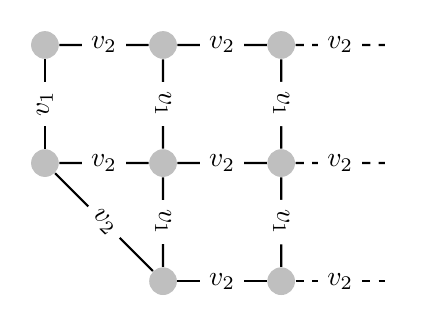
\begin{tikzpicture}[scale=\tikzpicscale]
%    \node[vertex] (00) at (0,0)   {};
    \node[vertex] (10) at (1,0)   {};
	 \node[vertex] (20) at (2,0)   {};
    \node[vertex] (01) at (0,1)   {};
    \node[vertex] (11) at (1,1)   {};
    \node[vertex] (21) at (2,1)   {};
    \node[vertex] (02) at (0,2)   {};
    \node[vertex] (12) at (1,2)   {};
    \node[vertex] (22) at (2,2)   {};
	 \Edge[label=$v_2$](01)(10)
	 \Edge[label=$v_2$](10)(20)
	 \Edge[label=$v_2$](01)(11)
	 \Edge[label=$v_2$](11)(21)
	 \Edge[label=$v_2$](02)(12)
	 \Edge[label=$v_2$](12)(22)	
%)	 \Edge[label=$v_1$](00)(01)
	 \Edge[label=$v_1$](10)(11)
	 \Edge[label=$v_1$](20)(21)
 	 \Edge[label=$v_1$](21)(22)
 	 \Edge[label=$v_1$](11)(12)
 	 \Edge[label=$v_1$](01)(02)
    \node[Nvertex] (n30) at (3,0)   {};
    \node[Nvertex] (n31) at (3,1)   {};
    \node[Nvertex] (n32) at (3,2)   {};
	 \tikzstyle{EdgeStyle}=[dashed]
	 \Edge[label=$v_2$](20)(n30)
	 \Edge[label=$v_2$](21)(n31)
 	 \Edge[label=$v_2$](22)(n32)
\end{tikzpicture}
}

\newcommand{\TIKZthreeladderC}{
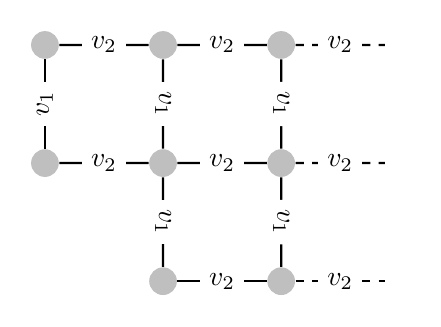
\begin{tikzpicture}[scale=\tikzpicscale]
%    \node[vertex] (00) at (0,0)   {};
    \node[vertex] (10) at (1,0)   {};
	 \node[vertex] (20) at (2,0)   {};
    \node[vertex] (01) at (0,1)   {};
    \node[vertex] (11) at (1,1)   {};
    \node[vertex] (21) at (2,1)   {};
    \node[vertex] (02) at (0,2)   {};
    \node[vertex] (12) at (1,2)   {};
    \node[vertex] (22) at (2,2)   {};
%	 \Edge[label=$v_2$](01)(10)
	 \Edge[label=$v_2$](10)(20)
	 \Edge[label=$v_2$](01)(11)
	 \Edge[label=$v_2$](11)(21)
	 \Edge[label=$v_2$](02)(12)
	 \Edge[label=$v_2$](12)(22)	
%)	 \Edge[label=$v_1$](00)(01)
	 \Edge[label=$v_1$](10)(11)
	 \Edge[label=$v_1$](20)(21)
 	 \Edge[label=$v_1$](21)(22)
 	 \Edge[label=$v_1$](11)(12)
 	 \Edge[label=$v_1$](01)(02)
    \node[Nvertex] (n30) at (3,0)   {};
    \node[Nvertex] (n31) at (3,1)   {};
    \node[Nvertex] (n32) at (3,2)   {};
	 \tikzstyle{EdgeStyle}=[dashed]
	 \Edge[label=$v_2$](20)(n30)
	 \Edge[label=$v_2$](21)(n31)
 	 \Edge[label=$v_2$](22)(n32)
\end{tikzpicture}
}

\newcommand{\TIKZthreeladderD}{
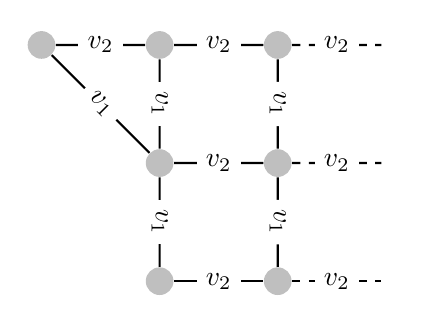
\begin{tikzpicture}[scale=\tikzpicscale]
%    \node[vertex] (00) at (0,0)   {};
    \node[vertex] (10) at (1,0)   {};
	 \node[vertex] (20) at (2,0)   {};
%    \node[vertex] (01) at (0,1)   {};
    \node[vertex] (11) at (1,1)   {};
    \node[vertex] (21) at (2,1)   {};
    \node[vertex] (02) at (0,2)   {};
    \node[vertex] (12) at (1,2)   {};
    \node[vertex] (22) at (2,2)   {};
%	 \Edge[label=$v_2$](01)(10)
	 \Edge[label=$v_2$](10)(20)
%	 \Edge[label=$v_2$](01)(11)
	 \Edge[label=$v_2$](11)(21)
	 \Edge[label=$v_2$](02)(12)
	 \Edge[label=$v_2$](12)(22)	
%)	 \Edge[label=$v_1$](00)(01)
	 \Edge[label=$v_1$](10)(11)
	 \Edge[label=$v_1$](20)(21)
 	 \Edge[label=$v_1$](21)(22)
 	 \Edge[label=$v_1$](11)(12)
 	 \Edge[label=$v_1$](11)(02)
    \node[Nvertex] (n30) at (3,0)   {};
    \node[Nvertex] (n31) at (3,1)   {};
    \node[Nvertex] (n32) at (3,2)   {};
	 \tikzstyle{EdgeStyle}=[dashed]
	 \Edge[label=$v_2$](20)(n30)
	 \Edge[label=$v_2$](21)(n31)
 	 \Edge[label=$v_2$](22)(n32)
\end{tikzpicture}
}

\newcommand{\TIKZthreeladderE}{
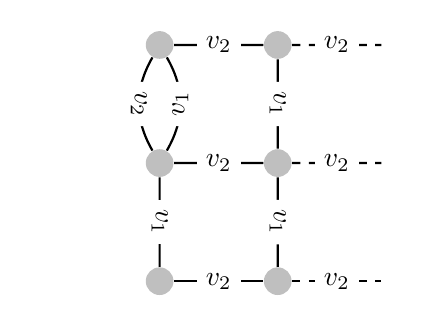
\begin{tikzpicture}[scale=\tikzpicscale]
    \node[Nvertex] (00) at (0,0)   {};
    \node[vertex] (10) at (1,0)   {};
	 \node[vertex] (20) at (2,0)   {};
%    \node[vertex] (01) at (0,1)   {};
    \node[vertex] (11) at (1,1)   {};
    \node[vertex] (21) at (2,1)   {};
%    \node[vertex] (02) at (0,2)   {};
    \node[vertex] (12) at (1,2)   {};
    \node[vertex] (22) at (2,2)   {};
%	 \Edge[label=$v_2$](01)(10)
	 \Edge[label=$v_2$](10)(20)
%	 \Edge[label=$v_2$](01)(11)
	 \Edge[label=$v_2$](11)(21)
%	 \Edge[label=$v_2$](02)(12)
	 \Edge[label=$v_2$](12)(22)	
%)	 \Edge[label=$v_1$](00)(01)
	 \Edge[label=$v_1$](10)(11)
	 \Edge[label=$v_1$](20)(21)
 	 \Edge[label=$v_1$](21)(22)
% 	 \Edge[label=$v_1$](11)(02)
    \node[Nvertex] (n30) at (3,0)   {};
    \node[Nvertex] (n31) at (3,1)   {};
    \node[Nvertex] (n32) at (3,2)   {};
	 \tikzstyle{EdgeStyle}=[dashed]
	 \Edge[label=$v_2$](20)(n30)
	 \Edge[label=$v_2$](21)(n31)
 	 \Edge[label=$v_2$](22)(n32)
 	 \tikzstyle{EdgeStyle}=[bend left]
  	 \Edge[label=$v_2$](11)(12)
  	 \tikzstyle{EdgeStyle}=[bend right]
  	 \Edge[label=$v_1$](11)(12)
\end{tikzpicture}
}

\newcommand{\TIKZthreeladderF}{
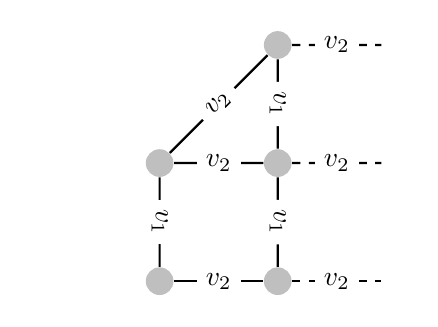
\begin{tikzpicture}[scale=\tikzpicscale]
    \node[Nvertex] (00) at (0,0)   {};
    \node[vertex] (10) at (1,0)   {};
	 \node[vertex] (20) at (2,0)   {};
%    \node[vertex] (01) at (0,1)   {};
    \node[vertex] (11) at (1,1)   {};
    \node[vertex] (21) at (2,1)   {};
%    \node[vertex] (02) at (0,2)   {};
%    \node[vertex] (12) at (1,2)   {};
    \node[vertex] (22) at (2,2)   {};
%	 \Edge[label=$v_2$](01)(10)
	 \Edge[label=$v_2$](10)(20)
%	 \Edge[label=$v_2$](01)(11)
	 \Edge[label=$v_2$](11)(21)
%	 \Edge[label=$v_2$](02)(12)
	 \Edge[label=$v_2$](11)(22)	
%)	 \Edge[label=$v_1$](00)(01)
	 \Edge[label=$v_1$](10)(11)
	 \Edge[label=$v_1$](20)(21)
 	 \Edge[label=$v_1$](21)(22)
% 	 \Edge[label=$v_1$](11)(02)
    \node[Nvertex] (n30) at (3,0)   {};
    \node[Nvertex] (n31) at (3,1)   {};
    \node[Nvertex] (n32) at (3,2)   {};
	 \tikzstyle{EdgeStyle}=[dashed]
	 \Edge[label=$v_2$](20)(n30)
	 \Edge[label=$v_2$](21)(n31)
 	 \Edge[label=$v_2$](22)(n32)
  	 %\tikzstyle{EdgeStyle}=[loop above]
  	 %\Edge[label=$v_1$](11)(11)
\end{tikzpicture}
}

\newcommand{\TIKZthreeladderG}{
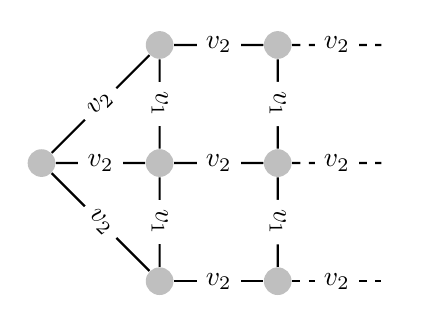
\begin{tikzpicture}[scale=\tikzpicscale]
%    \node[vertex] (00) at (0,0)   {};
    \node[vertex] (10) at (1,0)   {};
	 \node[vertex] (20) at (2,0)   {};
    \node[vertex] (01) at (0,1)   {};
    \node[vertex] (11) at (1,1)   {};
    \node[vertex] (21) at (2,1)   {};
%    \node[vertex] (02) at (0,2)   {};
    \node[vertex] (12) at (1,2)   {};
    \node[vertex] (22) at (2,2)   {};
	 \Edge[label=$v_2$](01)(10)
	 \Edge[label=$v_2$](10)(20)
	 \Edge[label=$v_2$](01)(11)
	 \Edge[label=$v_2$](11)(21)
	 \Edge[label=$v_2$](01)(12)
	 \Edge[label=$v_2$](12)(22)	
%)	 \Edge[label=$v_1$](00)(01)
	 \Edge[label=$v_1$](10)(11)
	 \Edge[label=$v_1$](20)(21)
 	 \Edge[label=$v_1$](21)(22)
 	 \Edge[label=$v_1$](11)(12)
% 	 \Edge[label=$v_1$](01)(02)
    \node[Nvertex] (n30) at (3,0)   {};
    \node[Nvertex] (n31) at (3,1)   {};
    \node[Nvertex] (n32) at (3,2)   {};
	 \tikzstyle{EdgeStyle}=[dashed]
	 \Edge[label=$v_2$](20)(n30)
	 \Edge[label=$v_2$](21)(n31)
 	 \Edge[label=$v_2$](22)(n32)
\end{tikzpicture}
}

\newcommand{\TIKZthreeladderH}{
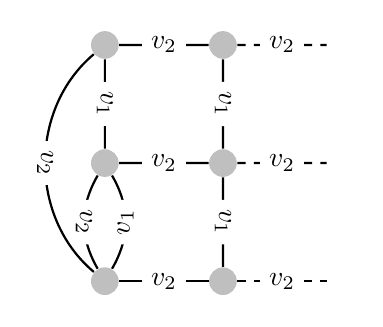
\begin{tikzpicture}[scale=\tikzpicscale]
%    \node[vertex] (00) at (0,0)   {};
    \node[vertex] (10) at (1,0)   {};
	 \node[vertex] (20) at (2,0)   {};
%    \node[vertex] (01) at (0,1)   {};
    \node[vertex] (11) at (1,1)   {};
    \node[vertex] (21) at (2,1)   {};
%    \node[vertex] (02) at (0,2)   {};
    \node[vertex] (12) at (1,2)   {};
    \node[vertex] (22) at (2,2)   {};
	 \Edge[label=$v_2$](10)(20)
%	 \Edge[label=$v_2$](01)(11)
	 \Edge[label=$v_2$](11)(21)
%	 \Edge[label=$v_2$](01)(12)
	 \Edge[label=$v_2$](12)(22)	
%)	 \Edge[label=$v_1$](00)(01)
	 \Edge[label=$v_1$](20)(21)
 	 \Edge[label=$v_1$](21)(22)
 	 \Edge[label=$v_1$](11)(12)
% 	 \Edge[label=$v_1$](01)(02)
    \node[Nvertex] (n30) at (3,0)   {};
    \node[Nvertex] (n31) at (3,1)   {};
    \node[Nvertex] (n32) at (3,2)   {};
	 \tikzstyle{EdgeStyle}=[dashed]
	 \Edge[label=$v_2$](20)(n30)
	 \Edge[label=$v_2$](21)(n31)
 	 \Edge[label=$v_2$](22)(n32)
 	 
 	 \tikzstyle{EdgeStyle}=[bend left]
 	 \Edge[label=$v_2$](10)(11)
  	 \tikzstyle{EdgeStyle}=[bend left=50]
 	 \Edge[label=$v_2$](10)(12)
  	 %\Edge[label=$v_2$](11)(12)
 	 \tikzstyle{EdgeStyle}=[bend right]
	 \Edge[label=$v_1$](10)(11)
\end{tikzpicture}
}

\newcommand{\TIKZthreeladderI}{
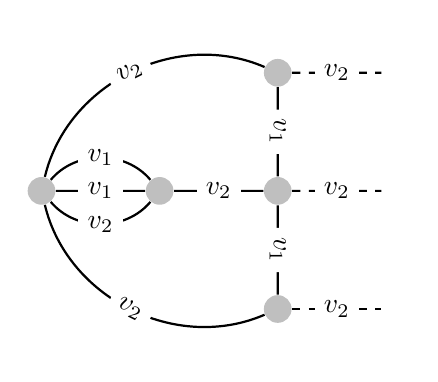
\begin{tikzpicture}[scale=\tikzpicscale]
%    \node[vertex] (00) at (0,0)   {};
%    \node[vertex] (10) at (1,0)   {};
	 \node[vertex] (20) at (2,0)   {};
    \node[vertex] (01) at (0,1)   {};
    \node[vertex] (11) at (1,1)   {};
    \node[vertex] (21) at (2,1)   {};
%    \node[vertex] (02) at (0,2)   {};
%    \node[vertex] (12) at (1,2)   {};
    \node[vertex] (22) at (2,2)   {};
%	 \Edge[label=$v_2$](01)(10)
%	 \Edge[label=$v_2$](10)(20)
%	 \Edge[label=$v_2$](01)(21)
	 \Edge[label=$v_2$](11)(21)
%	 \Edge[label=$v_2$](12)(22)	
%)	 \Edge[label=$v_1$](00)(01)
%	 \Edge[label=$v_1$](10)(11)
	 \Edge[label=$v_1$](20)(21)
 	 \Edge[label=$v_1$](21)(22)
% 	 \Edge[label=$v_1$](11)(12)
% 	 \Edge[label=$v_1$](01)(02)
    \node[Nvertex] (n30) at (3,0)   {};
    \node[Nvertex] (n31) at (3,1)   {};
    \node[Nvertex] (n32) at (3,2)   {};
	 \tikzstyle{EdgeStyle}=[dashed]
	 \Edge[label=$v_2$](20)(n30)
	 \Edge[label=$v_2$](21)(n31)
 	 \Edge[label=$v_2$](22)(n32)

	 \tikzstyle{EdgeStyle}=[]
	 \Edge[label=$v_1$](01)(11)
  	 \tikzstyle{EdgeStyle}=[bend left=50]
	 \Edge[label=$v_2$](01)(22)
 	 \Edge[label=$v_1$](01)(11)
  	 \tikzstyle{EdgeStyle}=[bend right=50]
 	 \Edge[label=$v_2$](01)(20)
 	 \Edge[label=$v_2$](01)(11)
\end{tikzpicture}
}


\newcommand{\TIKZthreeladderJ}{
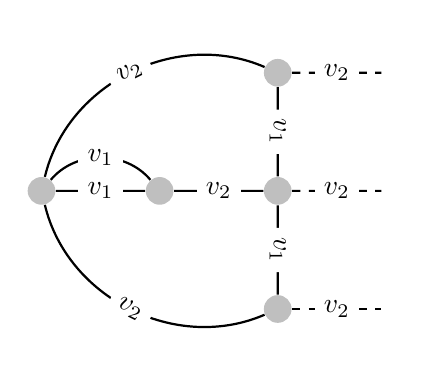
\begin{tikzpicture}[scale=\tikzpicscale]
%    \node[vertex] (00) at (0,0)   {};
%    \node[vertex] (10) at (1,0)   {};
	 \node[vertex] (20) at (2,0)   {};
    \node[vertex] (01) at (0,1)   {};
    \node[vertex] (11) at (1,1)   {};
    \node[vertex] (21) at (2,1)   {};
%    \node[vertex] (02) at (0,2)   {};
%    \node[vertex] (12) at (1,2)   {};
    \node[vertex] (22) at (2,2)   {};
%	 \Edge[label=$v_2$](01)(10)
%	 \Edge[label=$v_2$](10)(20)
%	 \Edge[label=$v_2$](01)(21)
	 \Edge[label=$v_2$](11)(21)
%	 \Edge[label=$v_2$](12)(22)	
%)	 \Edge[label=$v_1$](00)(01)
%	 \Edge[label=$v_1$](10)(11)
	 \Edge[label=$v_1$](20)(21)
 	 \Edge[label=$v_1$](21)(22)
% 	 \Edge[label=$v_1$](11)(12)
% 	 \Edge[label=$v_1$](01)(02)
    \node[Nvertex] (n30) at (3,0)   {};
    \node[Nvertex] (n31) at (3,1)   {};
    \node[Nvertex] (n32) at (3,2)   {};
	 \tikzstyle{EdgeStyle}=[dashed]
	 \Edge[label=$v_2$](20)(n30)
	 \Edge[label=$v_2$](21)(n31)
 	 \Edge[label=$v_2$](22)(n32)

	 \tikzstyle{EdgeStyle}=[]
	 \Edge[label=$v_1$](01)(11)
  	 \tikzstyle{EdgeStyle}=[bend left=50]
	 \Edge[label=$v_2$](01)(22)
 	 \Edge[label=$v_1$](01)(11)
  	 \tikzstyle{EdgeStyle}=[bend right=50]
 	 \Edge[label=$v_2$](01)(20)
% 	 \Edge[label=$v_2$](01)(11)
\end{tikzpicture}
}

\newcommand{\TIKZoneladderA}{
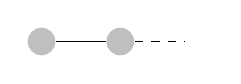
\begin{tikzpicture}[shorten >=1pt,->]
    \tikzstyle{vertex}=[circle,fill=black!25,minimum size=10pt,inner sep=2pt]
    \tikzstyle{nullvertex}=[circle,fill=white!25,minimum size=10pt,inner sep=2pt]
    \node[vertex] (G1) at (0,0)   {};
    \node[vertex] (G2) at (1,0)   {};
    \node[nullvertex] (GX) at (2,0)   {};
    \draw (G1) -- (G2) -- cycle;
    \draw[dashed] (G2) -- (GX) -- cycle;
\end{tikzpicture}
}

\newcommand{\TIKZoneladderB}{
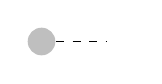
\begin{tikzpicture}[shorten >=1pt,->]
    \tikzstyle{vertex}=[circle,fill=black!25,minimum size=10pt,inner sep=2pt]
    \tikzstyle{nullvertex}=[circle,fill=white!25,minimum size=10pt,inner sep=2pt]
    \node[vertex] (G2) at (1,0)   {};
    \node[nullvertex] (GX) at (2,0)   {};
    \draw[dashed] (G2) -- (GX) -- cycle;
\end{tikzpicture}
}

\newcommand{\TIKZoneladderC}{

\begin{tikzpicture}[shorten >=1pt,->]
    \tikzstyle{vertex}=[circle,fill=black!25,minimum size=10pt,inner sep=2pt]
    \tikzstyle{nullvertex}=[circle,fill=white!25,minimum size=10pt,inner sep=2pt]
    \node[vertex] (G1) at (0,0)   {};
    \node[vertex] (G2) at (1,0)   {};
    \node[nullvertex] (GX) at (2,0)   {};
    %\draw (G1) -- (G2) -- cycle;
    \draw[dashed] (G2) -- (GX) -- cycle;
\end{tikzpicture}
}

\newcommand{\TIKZpetersengraph} {
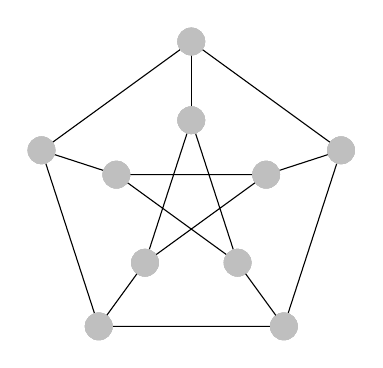
\begin{tikzpicture}[]
    \tikzstyle{vertex}=[circle,fill=black!25,minimum size=10pt,inner sep=2pt]
            
\draw (18:2cm) -- (90:2cm) -- (162:2cm) -- (234:2cm) -- (306:2cm) -- cycle;
\draw (18:1cm) -- (162:1cm) -- (306:1cm) -- (90:1cm) -- (234:1cm) -- cycle;
\foreach \x in {18,90,162,234,306}{
\draw (\x:1cm) -- (\x:2cm);

    \node[vertex] at (18:2cm) {};
    \node[vertex] at (90:2cm) {};
    \node[vertex] at (162:2cm) {};
    \node[vertex] at (234:2cm) {};
    \node[vertex] at (306:2cm) {};
    \node[vertex] at (18:1cm) {};
    \node[vertex] at (162:1cm) {};
    \node[vertex] at (306:1cm) {};
    \node[vertex] at (90:1cm) {};
    \node[vertex] at (234:1cm) {};

%\draw (\x:2cm) circle (2pt);
%\draw (\x:1cm) circle (2pt);
}
\end{tikzpicture}
}

\newcommand{\TIKZFLWmacrostates} {

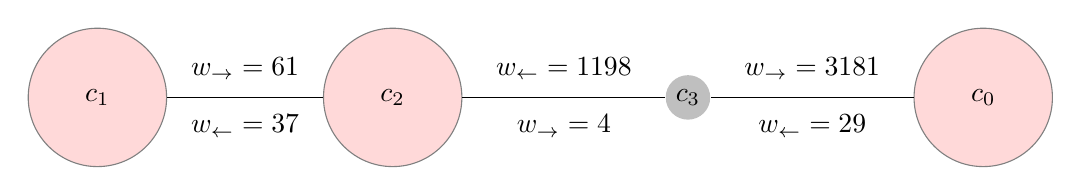
\begin{tikzpicture}[scale=\tikzpicscale]

  \node[big_vertex] (c1) at (0,0)   {$c_1$};
  \node[big_vertex] (c2) at (1*\vertexshiftamount,0)   {$c_2$};
  \node[vertex]    (c3) at (2*\vertexshiftamount,0)   {$c_3$};
  \node[big_vertex] (c0) at (3*\vertexshiftamount,0)   {$c_0$};
  
  \draw [] (c0) -> node[above=.1cm] {$w_{\rightarrow}=3181$} (c3);
  \draw [] (c0) -> node[below=.1cm] {$w_{\leftarrow}=29$} (c3);

  \draw [] (c2) -> node[above=.1cm] {$w_{\leftarrow}=1198$} (c3);  
  \draw [] (c2) -> node[below=.1cm] {$w_{\rightarrow}=4$} (c3);
  
  \draw [] (c2) -- node[below=.1cm] {$w_{\leftarrow}=37$} (c1);
  \draw [] (c2) -- node[above=.1cm] {$w_{\rightarrow}=61$} (c1);
\end{tikzpicture}
}

\newcommand{\TIKZbetahairpinNativestate} {
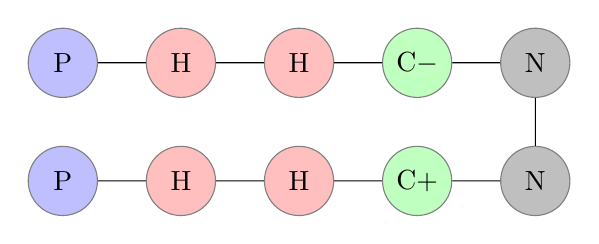
\begin{tikzpicture}[scale=\tikzpicscale]
    \tikzstyle{hvertex}=[circle,fill=red!25,minimum size=25pt,inner sep=2pt,draw=black!50]
    \tikzstyle{pvertex}=[circle,fill=blue!25,minimum size=25pt,inner sep=2pt,draw=black!50]
    \tikzstyle{cpvertex}=[circle,fill=green!25,minimum size=25pt,inner sep=2pt,draw=black!50]
    \tikzstyle{nvertex}=[circle,fill=black!25,minimum size=25pt,inner sep=2pt,draw=black!50]

    \node[pvertex] (r0) at (0,0)   {\chem{P}};
    \node[hvertex] (r1) at (1,0)   {\chem{H}};
    \node[hvertex] (r2) at (2,0)   {\chem{H}};
    \node[cpvertex] (r3) at (3,0)   {\chem{C+}};
    \node[nvertex] (r4) at (4,0)   {\chem{N}};
    \node[nvertex] (r5) at (4,1)   {\chem{N}};
    \node[cpvertex] (r6) at (3,1)   {\chem{C-}};
    \node[hvertex] (r7) at (2,1)   {\chem{H}};
    \node[hvertex] (r8) at (1,1)   {\chem{H}};
    \node[pvertex] (r9) at (0,1)   {\chem{P}};

    \draw [] (r0)--(r1)--(r2)--(r3)--(r4)--(r5)--(r6)--(r7)--(r8)--(r9)--cycle;
   
\end{tikzpicture}
}


\newcommand{\TIKZbetahairpinMacrostates} {
\begin{tikzpicture}[scale=\tikzpicscale]
    \node[macrostate_vertex] (R) at (0,0)   {
    \begin{minipage}{3.1cm}
    \includegraphics[width=1.5 cm]{supplement/beta_cluster_example_2/pictures/21/state_cluster_shapes_150.pdf} 
    \includegraphics[width=1.5 cm]{supplement/beta_cluster_example_2/pictures/21/state_cluster_shapes_17.pdf} \\
    \includegraphics[width=1.5 cm]{supplement/beta_cluster_example_2/pictures/21/state_cluster_shapes_32.pdf} 
    \includegraphics[width=1.5 cm]{supplement/beta_cluster_example_2/pictures/21/state_cluster_shapes_200.pdf} \\
  	 $c_\chem{R}$ random coil
    \end{minipage}
    };
    \node[macrostate_vertex] (I) at (1.5*\vertexshiftamount,0)   {
    \begin{minipage}{3.1cm} \centering
    \includegraphics[width=2 cm]{supplement/beta_cluster_example_2/pictures/saved_macrostates/intermed.png} \\
  	 $c_\chem{I}$ intermediate \\ (turn formation)
    \end{minipage}
	 };
    \node[macrostate_vertex] (F) at (3*\vertexshiftamount,0)   
    {
    \begin{minipage}{3.1cm} \centering
    \includegraphics[width=2.5 cm]{supplement/beta_cluster_example_2/pictures/saved_macrostates/native.png} \\
  	 $c_\chem{F}$ native state
    \end{minipage}
    };

  \tikzstyle{EdgeStyle}=[bend right]
  \Edge[label=$\B{S}_{\chem{R I}}$](R)(I)
  \Edge[label=$\B{S}_{\chem{I R}}$](I)(R)
  
  \tikzstyle{EdgeStyle}=[]
  \Edge[label=$\B{S}_{\chem{I F}}$](I)(F)
  
\end{tikzpicture}
}


%\end{comment}


\begin{document}
\suppressfooter{}
\begin{preamble}

\iffinal{}{\newpage}

\begin{DUTdedications}
%
\vspace*{\fill}
%
\begin{center}
\setstretch{2}
\begin{minipage}{8 cm}
\begin{center}
\hrulefill\\

This thesis is dedicated to my family. Their unconditional support and love was
the foundation of success for my graduate study. I want you to know that I love
you so much and this thesis was only possible thanks to you. 

\hrulefill
\vspace{6em}
\end{center}
\end{minipage}
\end{center}
\vspace*{\fill}
\end{DUTdedications}

\iffinal{}{\newpage}

\begin{acknowledgments}
%Over the past six years I have received support and encouragement form many
    %people.

This dissertation summarized the research work I have accomplished during my
graduate study in Drexel University. Over all these years, I obtained
tremendous help from all the people around and I cannot leave the dissertation
without expressing my gratitude to them.

This work would not have been possible without the support of my advisor, Dr.
Bahram Nabet. His guidance helped to shape and provided much needed focus to my
work.  I would also like to thank my dissertation committee of Dr. Timothy Kurzweg,
Dr. Baris Taskin, Dr. Nagarajan Kandasamy, and Dr. Goran Karapetrov for their
support and insight throughout my research.

Many thanks to our generous collaborators, Dr. Adriano Cola, Dr. Anna Persano,
Dr. Paola Prete at IMM-NCR in Italy, Dr. Nico Lovergine at University of
Salento in Italy and Dr. Marc Currie from Navel Research Laboratory in
Washington D.C. for their tremendous efforts in fabrication of the AlGaAs/GaAs
core-shell nanowires and electro-optically sampling, micro-photoluminescence
measurements of the devices. Although, I have not had the opportunity of
meeting them yet, it is still a great pleasure to communicate with them in
Email and I appreciate their valuable thoughts and discussions in many of the
experimental results. I would also like to dedicate many thanks to Dr. Fernando
Camino, Dr. Aaron Stein, Dr. Chang-Yong Nam, Dr. Mircea Cotlet and many other
staffs at CFN of Brookhaven National Laboratory in Long Island for their
assistance and suggestions in characterizing the devices.

I would also like to thank my friends in the Photonics Lab for all the help and
support they provided, and especially for providing such a friendly and awesome
place to work and study at. Pouya Dianat, Weston Aenchbacher and Shrenik Vora
have spent countless hours listening to me talk about my research, helping me
flesh out my ideas. And a special thanks to Jiajia Liu for accompanying me
during all these years and bringing countless happiness to my life.

Finally, my parents deserve my most sincere gratitude. I appreciate you spent
one or two months each year to be in the states with me, and they always
believe in, encourage and love me even when they live on the other side of the
earth.

\end{acknowledgments}

\iffinal{}{\newpage}

\tableofcontents 
\iffinal{}{\newpage}

\listoftables
\iffinal{}{\newpage}

\listoffigures 
\iffinal{}{\newpage}

\begin{abstract}
%\ifdaring{\setstretch{1.3}}{}
\ifdaring{\setstretch{1.3}}{\setstretch{1.6}}

Semiconductor nanowires have been used in a variety of passive and active
optoelectronic devices including waveguides, photodetectors, solar cells, LEDs,
Lasers, sensors, and optical antennas. We have designed and fabricated
GaAs/AlGaAs core-shell nanowires (CSNWs) grown on both GaAs and Si substrates
by vapor-liquid-solid (VLS) method. These nanowires show extremely enhanced
optical properties in terms of absorption, guiding, radiation of light, and
even lasing. Analysis of the interaction of light with cylindrical and
hexagonal structures with sub-wavelength diameters identifies both transverse
plane modes and longitudinal plane modes in a generalized volumetric resonance
modes without the need for vertical structures such as Bragg mirrors commonly
used in vertical cavity surface emitting lasers (VCSEL's). We report on FDTD
simulations with the aim of identifying the dependence of these modes on:
geometry (length, width), tapering, shape (cylindrical, hexagonal), core-shell
versus core-only, and dielectric cores with semiconductor shells. This
demonstrates how NWs form excellent optical cavities without the need for top
and bottom mirrors. However, optically equivalent structures such as hexagonal
and cylindrical wires can have very different optoelectronic properties meaning
that light management alone does not sufficiently describe the observed
enhancement in upward (absorption) and downward transitions (emission) of light
in nanowires; rather, the electronic transition rates should be considered. We
discuss how the transition rates change with respect to electron distribution
and identify three factors explicitly contributed to the transition rates with
strong dependence on dimensionality. In addition, a CSNW based laser has been
proposed and modeled, showing large increase in optical gain and quantum
efficiency compared to their bulk counterparts. These results and findings will
further facilitate the design and optimization of sub-micron scale
optoelectronic devices. In conclusion, we make a case for photonic integrated
circuits that can take advantage of the confluence of the desirable optical and
electronic properties of these nanostructures.

\end{abstract}

\iffinal{}{\newpage}

\end{preamble}


\begin{thesis}
  \pdfbookmark[-1]{Main Matter}{Main Matter}
  \ifdaring{\setstretch{1.3}}{}
  %\ifdaring{\setstretch{1.3}}{\setstretch{1.3}}
  
  \restorefooter{}

  %CHAPTER: Introduction
  \chapter{Introduction}

The development of sophisticated growth techniques for layered semiconductor
structures has stimulated a large body of new work in semiconductor physics
over the last fifteen years or so. Undoubtedly, much of this interest was
further stimulated by the possibility of novel physics and applications in
electronic transport. New physical discovered in inversion channels and
heterostructures, and the first heterostructure electronic devices, such as
modulation-doped field-effect transistors and heterojuntion bipolar
transistors, are now being commercially exploited. Linear optical spectroscopic
techniques, such as absorption, luminescnence and modulation spectroscopy, have
for a long time been important tools in understanding the basic physics of
semiconductor materials. Also over the last fifteen years or so, semiconductor
optical and optioelectronic properties have become of increasing technological
importance in their own right. The ever-growing application of semiconductor
diode lasers and related optoelectronic technology in communications and
consumer products has helped to give yet further impetus to research on
semiconductor optical properties. 

The successes of semiconductor optoelectronics and promising physical
mechanisms and novel devices using quantum-confined structures have,
furthermore, enlivened the debate over possible applications of optics for
other functions such as logic and switching in communications and computation.

It is important to emphasize at the outset that quantum confinement and produce
not only quantitative but also qualitative differences in physics from that in
bulk structures, which is of course another major motivation for the interest
in them. There are many examples of these differences. The optical absorption
spectrum breaks up into a series of steps associated with the quantum-confined
electron and hole levels. Excitonic effects become much stronger because of the
quantum confinement, giving clear absorption resonances even at room
temperature. The relative importance of direct Coulomb screening and exchange
effects is quite different in quantum wells (the Coulomb screening is
relatively much weaker), giving very different optical saturation behaviour.

\section{Background} \label{sec:AD}


%\subsection{$\alpha$--Disk Model}


%\subsection{Eddington Luminosity} \label{Eddington_fraction}


%\section{Spectral Energy Distributions}


\section{Problem Statement} \label{sec:dust_intro}

\section{Literature Review} \label{sec:intro_MBH}


\section{Outline of Chapters}

This thesis is structured as follows. The data used for this analysis are presented in Chapter~\ref{data}.  After introducing the corrections and data analysis methods, Chapter~\ref{SEDs} presents our findings for individual and mean bolometric corrections.  Chapter~\ref{Dust} presents our methods and findings for estimating dust reddening associated with a subset of our quasars.  The statistical methods used in this chapter are outlined in more detail in Appendix~\ref{ch:mcmc}. In Chapter~\ref{BH}, we apply the corrections from Chapter~\ref{Dust} to our SEDs and use estimated black hole masses to study changes in the SEDs with the properties of the central black hole. Finally, we present our conclusions in Chapter~\ref{conclusions}. Throughout this work we use a $\Lambda$CDM cosmology with $H_0=71$ km s$^{-1}$ Mpc$^{-1}$, $\Omega_\Lambda = 0.734$, and $\Omega_m = 0.266$, consistent with the {\em Wilkinson Microwave Anisotropy Probe} 7 cosmology \citep{Jarosik:2011}.


  
  %CHAPTER: Experimental Results
  \chapter{Optical Enhancement of Core-Shell Nanowire} \label{data}

Given that the profound enhancement of optoeletronic properties of nanowires is
the major theme of this dissertation, it is dutiful to first summarize the
major experimental results, such as fabrication and characteristics of
core-shell nanowires (CSNWs).

Electron systems in lower dimensions are adequately treated through
perturbation methods. For 1D electron systems (1DES) the correlations among
electrons are much more significant due to higher degrees of confinement. The
electron can either be moving to the left or right and any small or localized
interaction can cause a collective response from the whole system. This is the
condition of broken symmetry, in which the overall status of the system has to
be reformulated. For a 2DES, a broken symmetry occurs at very low densities of
fermions, in which formation of a Wigner lattice is expected, which is due to
the Coulombic interactions of electrons. Interestingly for a 1DES, the
direction of movement for fermions is restricted to the left or right.
Consequently, the density of the system becomes irrelevant with respect to the
determination of the status of the system. Such a 1D many electron system is
often called a $L\ddot{u}finger$ Liquid, as he was the first person who
successfully formulated these systems.

Importantly, a 1DES can experimentally be realized in various material systems.
These include carbon nanotubes, electrons at the edges of a 2DES, and in
nanowires.

A core-shell nanowire (CSNW) is a quasi-one dimensional structure with a wide
band gap materials, such as AlGaAs, wrapping around a low band gap
semiconductor, such as GaAs.

It is expected that the lower dimensionality in CSNW to have a significant
influence on both optical and electrical properties of the structure. Fot
instantce,

Electrically it is important account for the electron correlations in order to
determine the behavior of the structure. The significant values of exchange
and correlation energies in 1DES, makes them an interesting candidate for
probing their energy dynamics. This, however, imposes various experimental
challenges and theoretical considerations and are deferred to future
investigations.

\section{Growth of Nanowires}

Freestanding quasi-one-dimensional semiconductor nanostructures (nanowires)
based on III-V compound semiconductors, owing to their unique physical
properties, are considered ideal building blocks for the realization of
photonic and electronic nanodevices.

Currently, two bottom-up approaches to the fabrication of freestanding
nanowires are considered: (i) selective area epitaxy
(SAE)~\cite{motohisa2004catalyst} and (ii) metal-catalyst assisted grouth
through the so-called vapor-liquid-solid (VLS) mechanism~\cite{wagner1964vapor,
givargizov1975fundamental}. The latter method relies on the alloying of a metal
catalyst (usually Au) nanoparticle with the semiconductor constituent elements,
supplied through a vapor phase. The as-formed alloy acts as an initial
nucleation site for the material and further guides the nanowire growth, the
diameter of the nanowire being controlled by that of the metal nanoparticle.

An advantage of the VLS method over SAE is that it does not require
nanolithograpic processing of the substrate; furthermore, it is compatible with
most advanced epitaxial grouth techniques for III-V compounds, such as
molecular beam epitaxy, chemical beam epitaxy, and metalorganic vapor phase
epitaxy (MOVPE). 

GaAs nanowires were grown by low (50mbar) pressure MOVPE using an Aixtron
reactor model AIX200 RD. TMGa and TBAs were used as gallium and arsenic
precursors, respectively. Au nanoparticle deposited on
$(\bar{1}\bar{1}\bar{1})B$ GaAs were used to catalyze the nanowire growth. To
this purpose, VGF-grown semi-insulating (undoped) GaAs wafers oriented
$(\bar{1}\bar{1}\bar{1})B$ were used. The substrates were then first degreased
in isopropanol vapors, etched in $4H_2SO_4:1H_2O_2:2H_2O$ solution for 8 min at
around $40\,^{\circ}\mathrm{c}$, ringsed in de-ionized water and finally dried
under pure $N_2$. Au nanoparticles with $\sim 60 nm$ diameters were prepared by
reaction of $HAuCl_4$ with sodium citrate in aqueous solution and randomly
deposited on the as-prepared GaAs surface by dropping a small amount of
colloidal solution onto the substrate. The solvent (water) was then evaporated
by holding the samples on a hot plate (in air) or a few minutes; Au
nanoparticle surface densities thus achieved ranged around (1-4). 

After loading the sample into the reactor chamber, its temperature was raised,
and sample annealing was then performed for 10 min to absorb GaAs surface
oxides and organic residues originating from the Au nanoparticle synthesis.
This annealing step would also allow the initial uptake of Ga atoms from the
GaAs substrate into the Au nanoparticles. 

\section{Scanning Electron Microscopy Images} 

Figure~\ref{SEMNW} is top view scanning electron microscopy (SEM) image of
nanowires of with $\sim100nm$ diameter core of GaAs, and $\sim40nm$ thick
AlGaAs, with the four figures showing at different magnifications and view
angles. These images demonstrate the rather sparse distribution of the wires.
In addition, the wires are not fully arrayed with various growth directions and
lengths. The most magnified view for the left bottom figure clearly indicate
the CSNWs have hexagonal structure and tapering effect along the wire growth
direction.

\begin{figure}
  \caption{Scanning Electron Microscopy image of as-grown GaAs/AlGaAs core-shell nanowires on Si taken at different magnifications and view angles (Image courtesy of Dr.Pouya Dianat)}
  \centering
  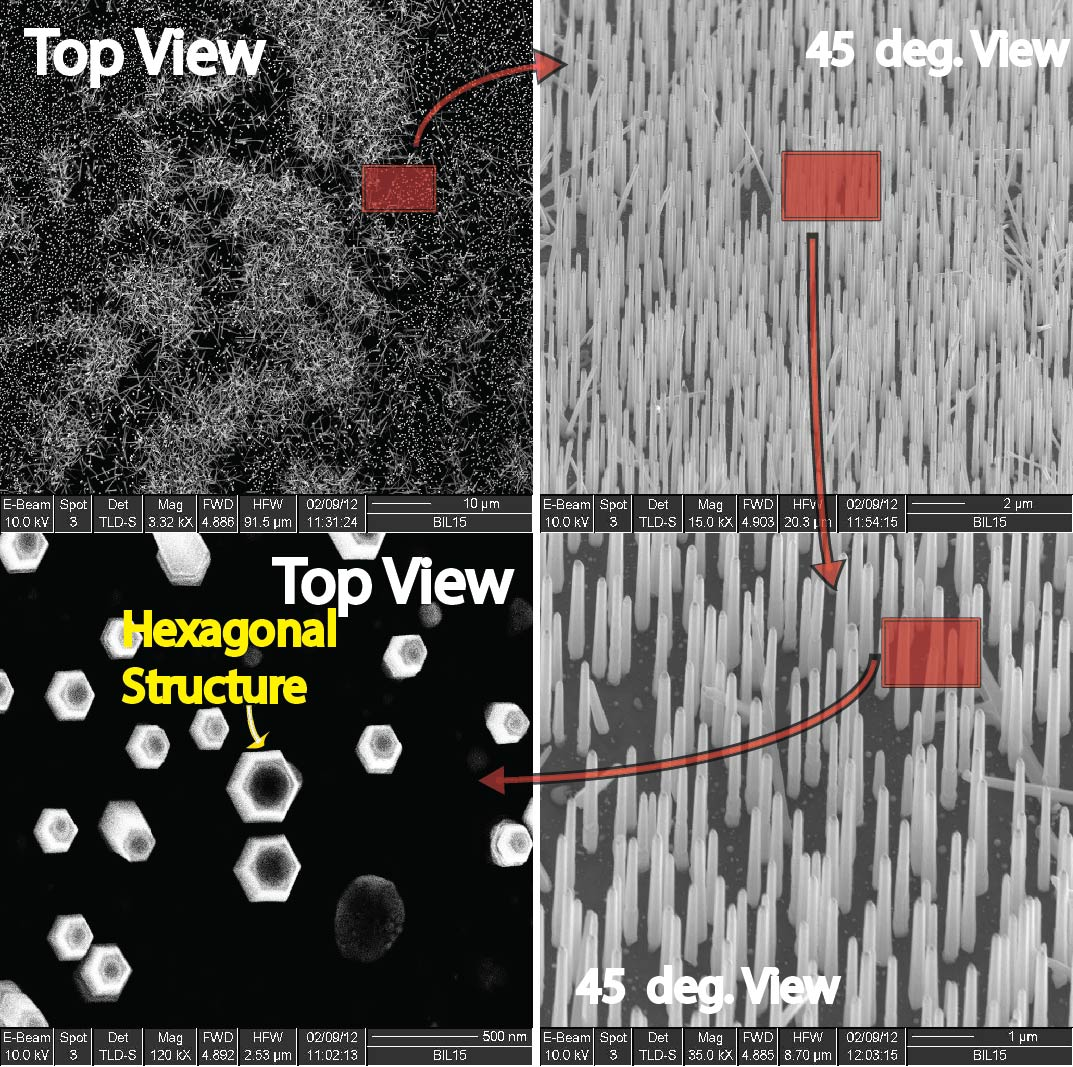
\includegraphics[width=\textwidth]{pictures/Data/SEMNW}
  \label{SEMNW}
\end{figure}

\section{Electrical Characterization of Nanowire}

The as-grown CSNWs are used to perform optical characterization measurement.
However, in order to measure the CSNWs electrical performance, additional
treatments have been taken to make Ohmic contacts between nanowires and
transmission lines.

Characteristic current-voltage (I-V) curves of the nanowire device are given in
Fig.~\ref{CSNWIV_light}. The I-V curve exhibits rectifying behavior, confirming
that the device is a well=behaved diode structure with the electric contact on
one side (Al) ohmic and the other (Pt) Schottky. The reverse bias dark current
of the device is very small, $\sim20pA$ at -1V, and could be further improved
by properly passivating the CSNW surface. Upon illumination, the device shows a
prnounced photovoltaic response due to the built-in potential from the Schottky
junction. The short length of the nanowire device and the large depleted region
by the built-in potential enable the nanowire photodetector to be operated at
zero bias. Fig.~\ref{CSNWIV_light} shows the photocurrent of the device at zero
bias as a function of irradiance. The linearity of the device was demonstrated
up to at least at a 632 nm wavelength. The excellent linear response is in part
based on the good crystalline quality of the nanowires, as confirmed by
transmission electron microscopy. In addition, the capactiance of a typical
device () is calculated to be 5 aF based on a simple parallel-plate model and
thus its cutoff frequency is mainly limited by the transit time of the
photo-generated charge carriers in the device, which may in principle reach ~
100 GHz after certain parameter opti 

\begin{figure}
  \caption{Scanning Electron Microscopy (SEM) image of one dispersed core-shell nanowire connecting with the transmission line by Focus Ion Beam (FIB).}
  \centering
  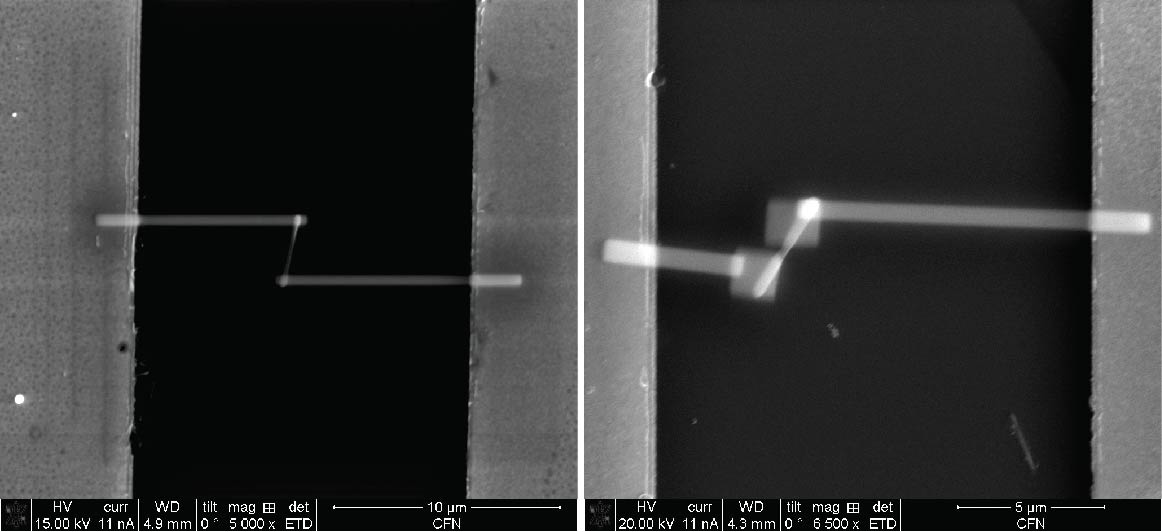
\includegraphics[width=\textwidth]{pictures/Data/ContactNW}
  \label{ContactNW}
\end{figure}

\begin{figure}
  \caption{Current versus Voltage Measurement under illumination of Single Core-Shell Nanowire.}
  \centering
  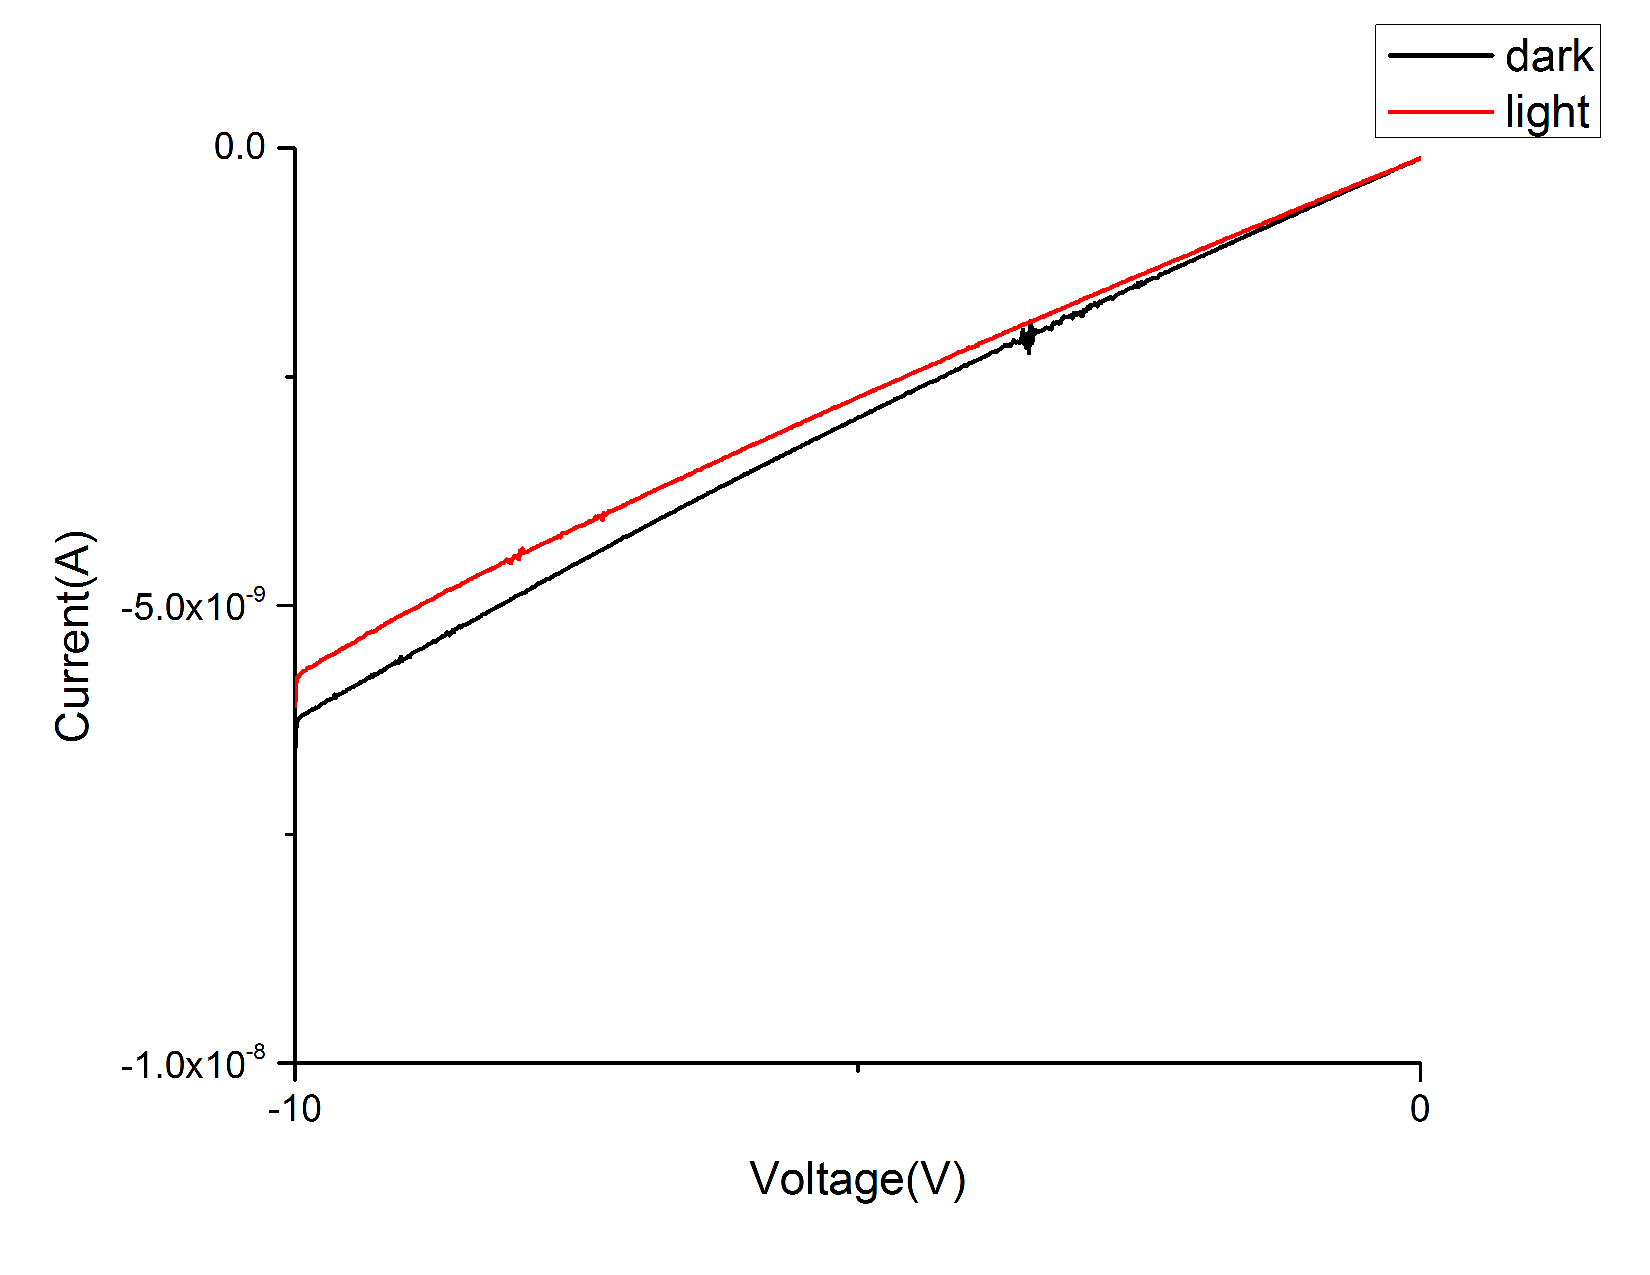
\includegraphics[width=\textwidth]{pictures/Data/CSNWIVlight}
  \label{CSNWIVlight}
\end{figure}

\begin{figure}
  \caption{Capacitance versus Voltage Measurement under illumination of Single Core-Shell Nanowire.}
  \centering
  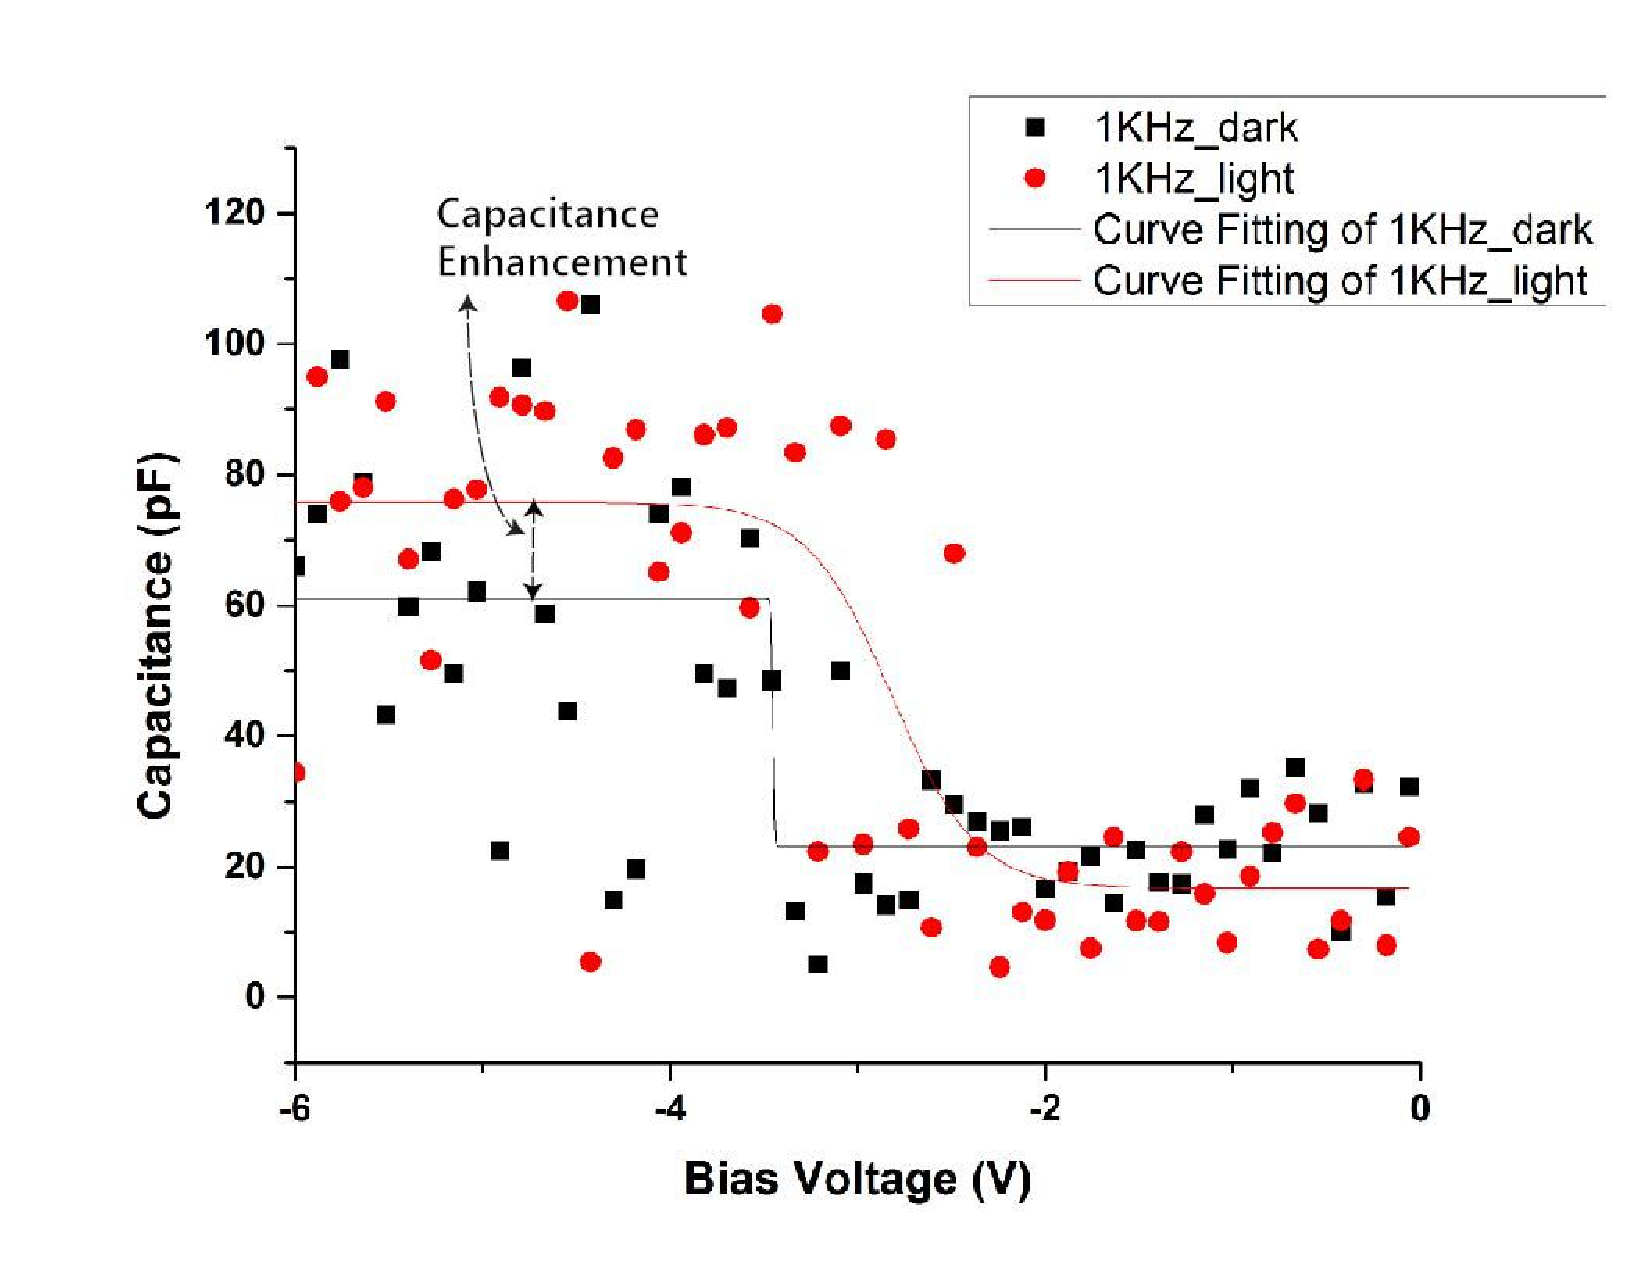
\includegraphics[width=\textwidth]{pictures/Data/CSNWCVlight}
  \label{CSNWCVlight}
\end{figure}

\section{Absorption Enhancement} \label{Data_Abs}

Figure~\ref{reflecbulk} shows the reflectivity of a GaAs wafer on which 50 nm
thin film of AlGaAs is grown, and compared this to the reflectivity spectrum of
a Si substrate. As expected, about 30\% to 55\% of a normally incident light is
reflected in bulk Si and GaAs, with a sharp change for wavelengths near their
respective band gaps. All the data are normalized to the reflectivity of gold
(Au).

\begin{figure}
  \caption{Reflectivity of GaAs (blue) and Si (green) substrates measured with $\sim{\mu}m$ normally incident beam.}
  \centering
  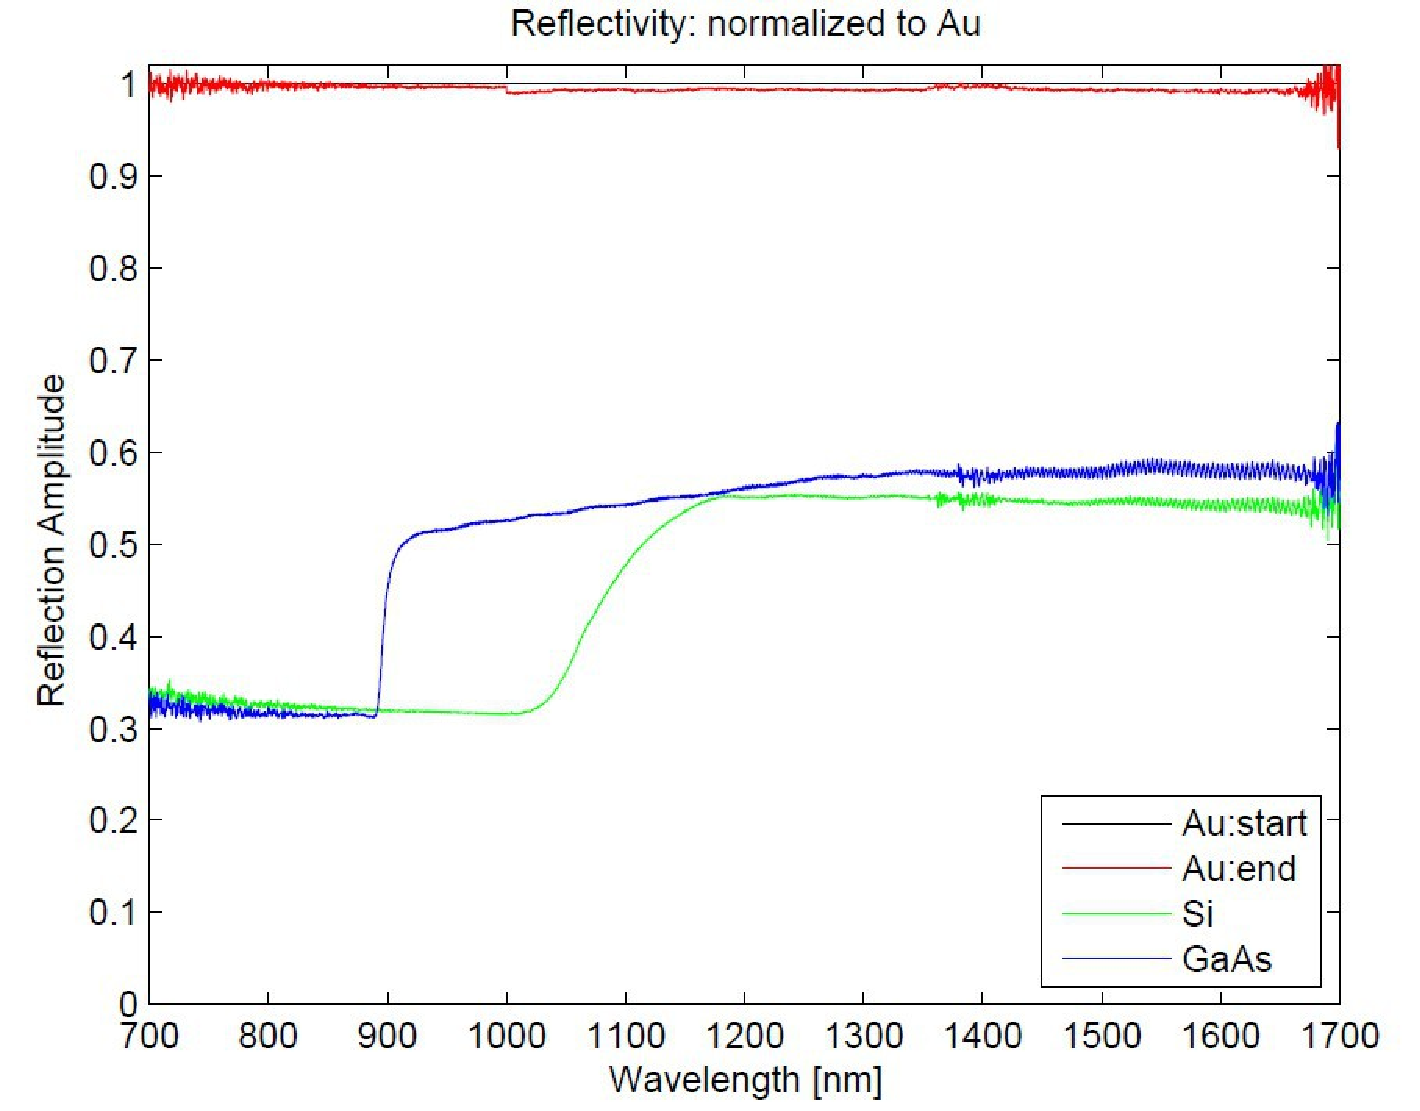
\includegraphics[width=\textwidth]{pictures/Data/reflecbulk}
  \label{reflecbulk}
\end{figure}

Figure~\ref{reflectCSNW} contrasts this with the measured absorption spectrum
of two types of GaAs core, AlGaAs shell nanowires (CSNWs): those grown on a
GaAs substrate (black), and the others heteroexpitaxially grown on a Si
substrate (red). The spectra show that both cases have the signature change of
reflectivity at badgap of GaAs, i.e., these are due to the GaAs/AlGaAs CSNWs,
not the substrate. Importantly, for the wavelength range of 700-1200nm these
core-shells which only occupy ~15\% of the volume compared to thin films of the
same height, reflect 2-4\% of light for the CSNWs grown on Si, and 3-7\% of
light for those grown on GaAs substrate. The beam-width of the incident light
being $\sim1{\mu}m$, this shows that only a few NWs are interrogated by ligth
and, normalized to volume, these wires absorb more than two orders of magnitude
more ligth than their thin-film counterparts.

\begin{figure}
  \caption{Reflectivity spectrum of GaAs/AlGaAs core-shells grown on Si (red) and GaAs (black) substrates shows, normalized to volume, nearly two orders of magnitude more absorption of ligth.}
  \centering
  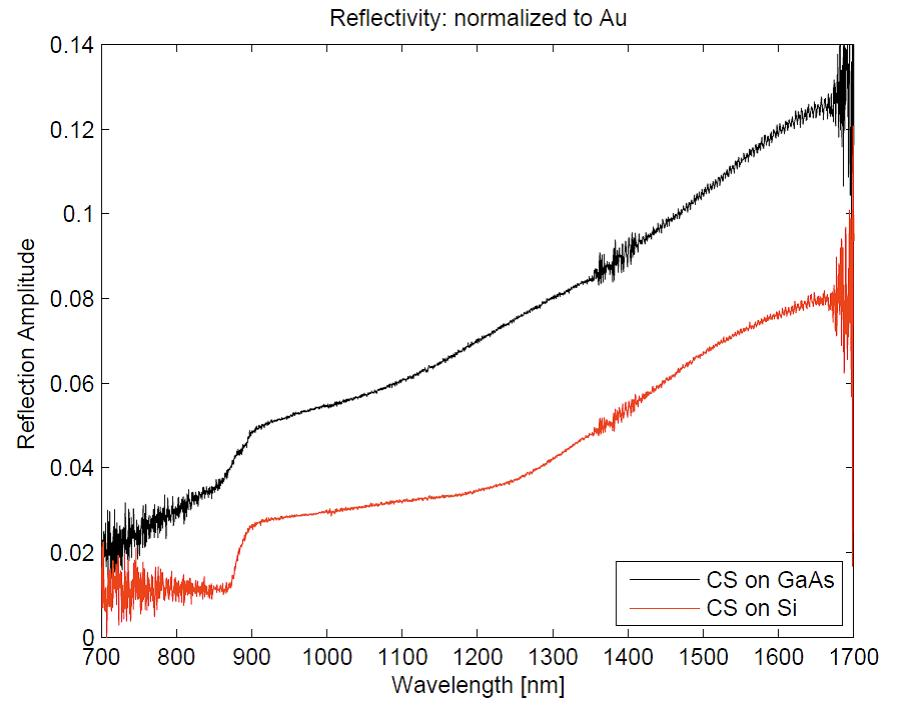
\includegraphics[width=\textwidth]{pictures/Data/reflectCSNW}
  \label{reflectCSNW}
\end{figure}

\section{Emission Enhancement} \label{Dust_data}

Figure~\ref{PL} compares room temperature micro photoluminescence (PL) spectrum
of bulk GaAs to CSNWs grown on GaAs, and two cuts of Si. The ratio of peak
luminescence of a) CSNWs on GaAs, B) CSNWs on Si[111] and c) Si(miscut)
substrates to bulk GaAs are, respectively, 923, 311 and 10. Considering the
beam width of $\sim1{\mu}m$, 5-10 NW were excited, yet emitted over three
order of magnitude more light compared to bulk.

\begin{figure}
  \caption{Photoluminescence of bulk GaAs, Core-Shell Nanowires grown on GaAs and Si.}
  \centering
  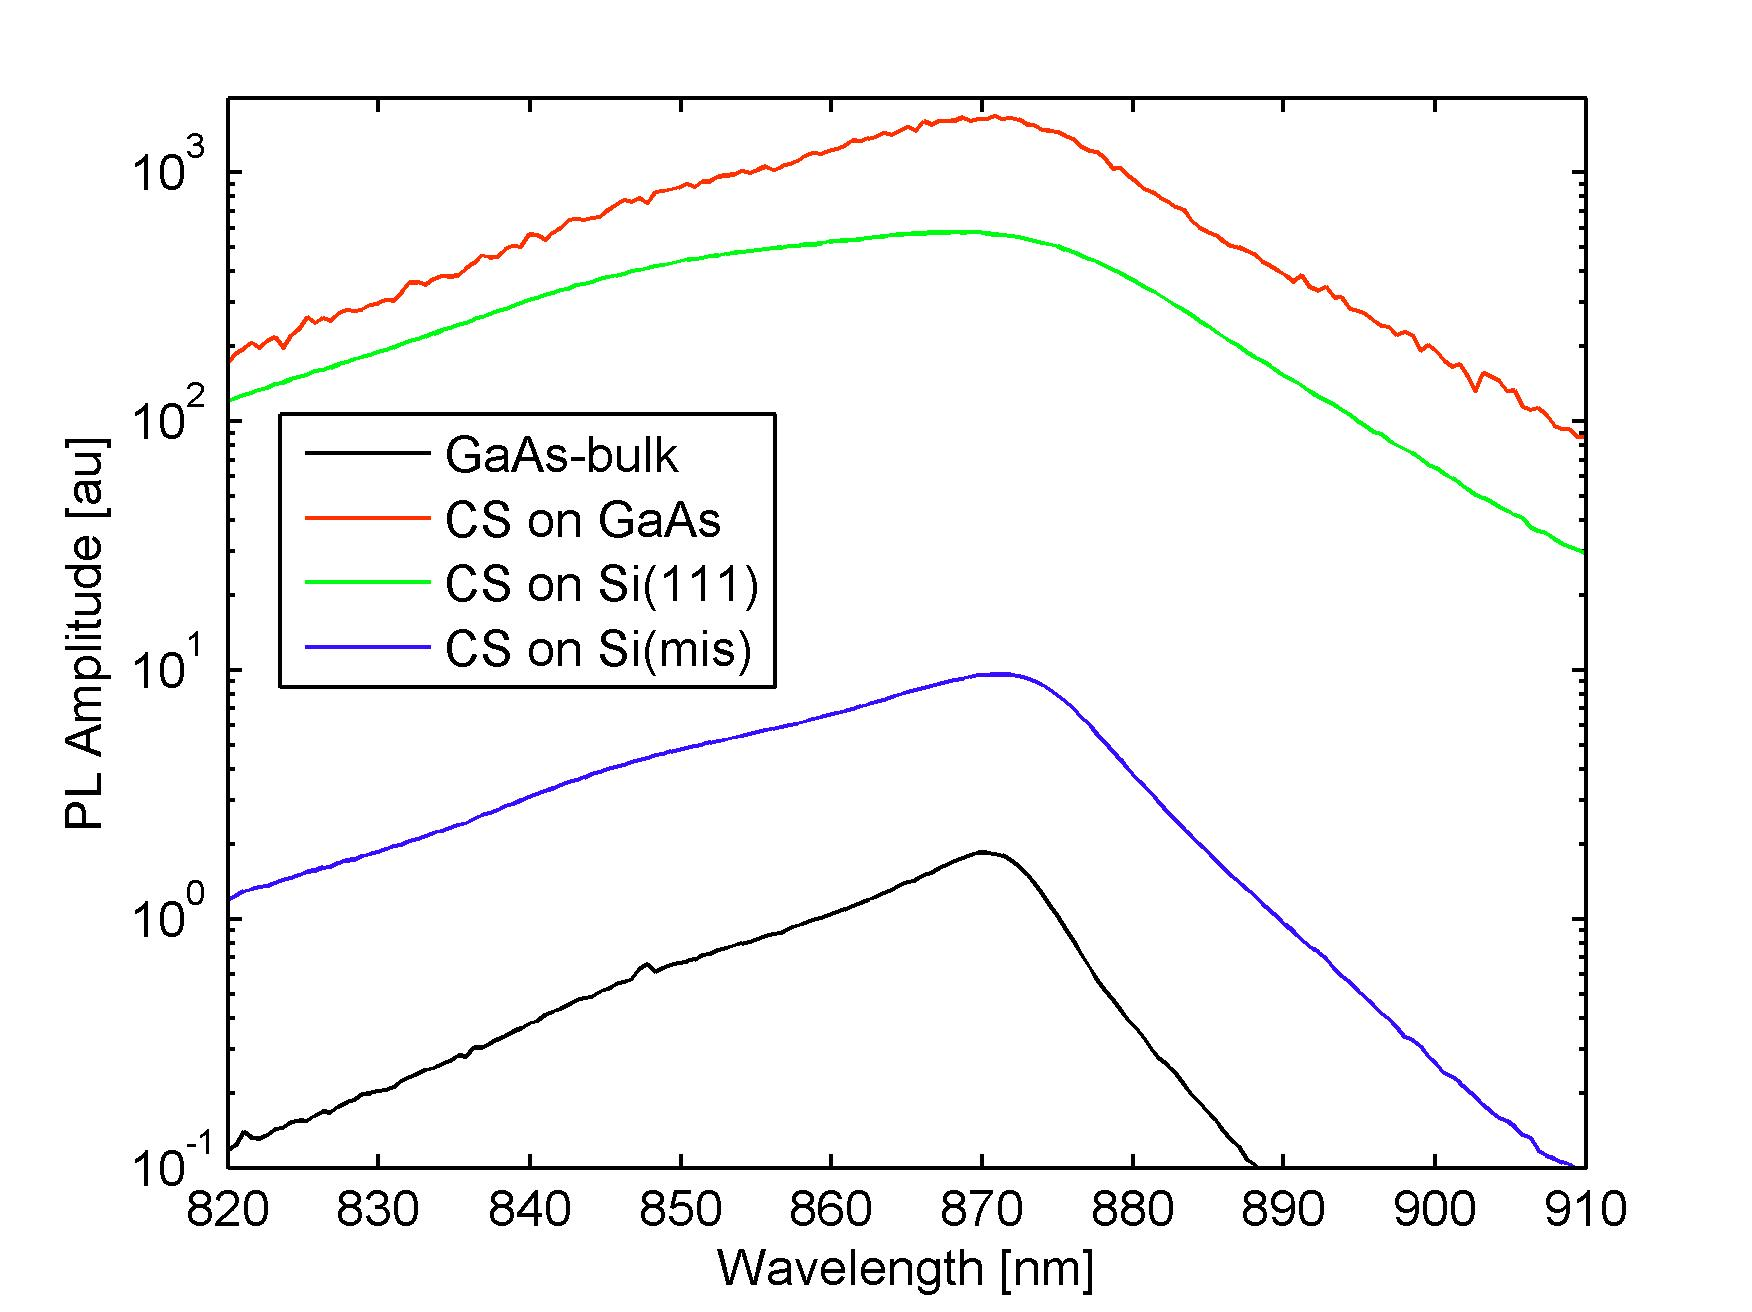
\includegraphics[width=\textwidth]{pictures/Data/PL}
  \label{PL}
\end{figure}

\section{Lasing} \label{data_lasing}

Photoluminescence (PL) of bulk GaAs to CSNWs grown on GaAs, and on two
directions of Si showed that normalized to the fraction of the volume that
these wires occupy, nearly 10,000 times more brightness is observed in these
wires compared to thin-film as in Fig.~\ref{PL}. In the case of stimulated
emission of light, the photon mode density $(1+u_\varepsilon)$ plays a crucial
role. Figure ~\ref{lasing} is the photoluminescence (PL) spectrum at various
optical pump intensities. As the excitation laser power increase beyond
$5{\mu}W$ a sudden and highly nonlinear increase in the emission intensity is
observed, with pronounced peaks emerging from 800nm to 850nm that rapidly grows
to become several orders of magnitude stronger than the background emission.
The lasing amplitude versus excitation power demonstrates a threshold of around
$5{\mu}W$, followed by saturation near $12{\mu}W$. This nonlinear threshold
behavior shows in detail in the L-L plot, (i.e., The pumping power intensity
(L) versus output light power intensity (L)) as in Fig.~\ref{expthreshold}. The
sharp peak has a full width half maximum (FWHM) that varies from 1.5 to 3.5 nm.
This remarkable behavior is achieved in the as-grown wires with no vertical
structure.

\begin{figure}
  \caption{Micro-Photoluminescence measurements with fs-pulsed, 532-nm laser excitation at 250kHz repetition rate shows lasing of the as-grown wires.}
  \centering
  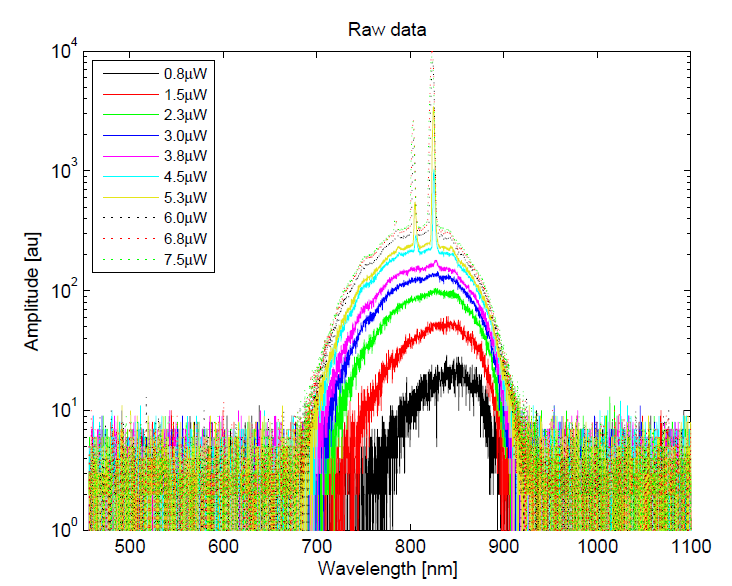
\includegraphics[width=\textwidth]{pictures/Data/lasing}
  \label{lasing}
\end{figure}

\begin{figure}
  \caption{\em{L-L curve of as-grown core-shell nanowire.} The pumping power intensity (L) versus output light power intensity (L) of as-grown core-shell nanowire operating at room temperature with a low threshold of $\sim10{\mu}W$ and followed by saturation near $22{\mu}W$.}
  \centering
  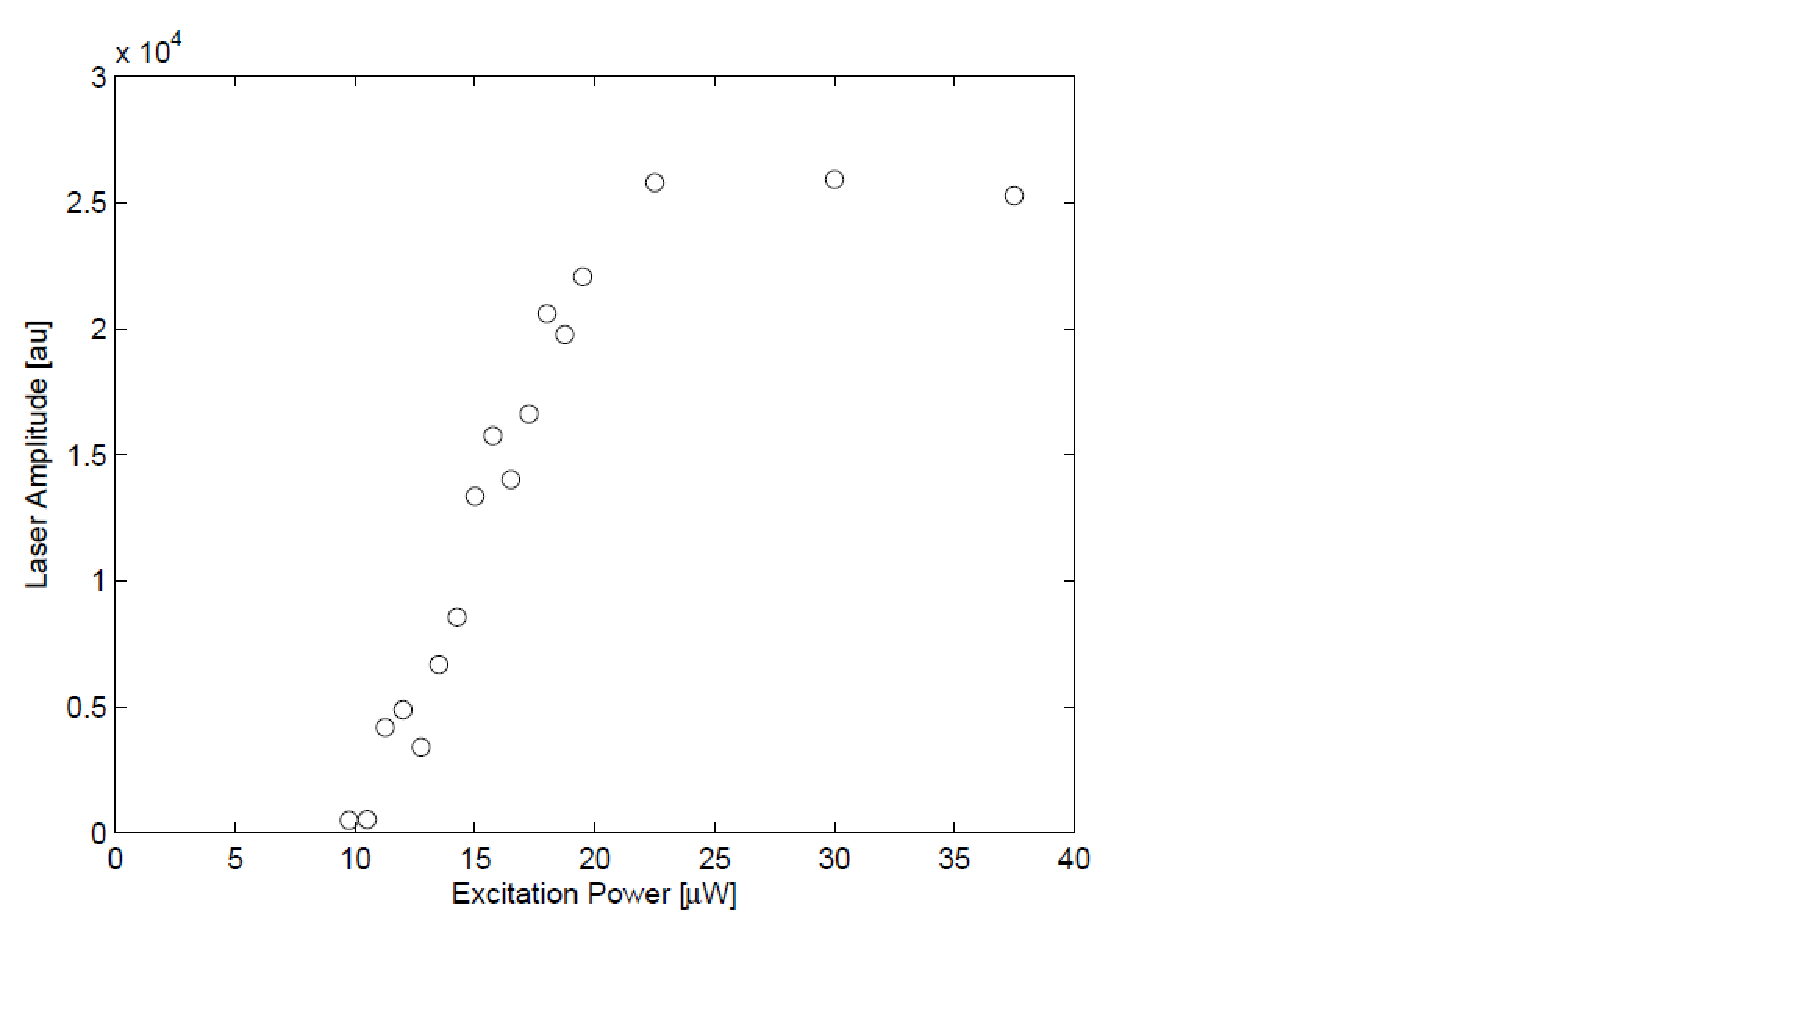
\includegraphics[width=\textwidth]{pictures/Data/expthreshold}
  \label{expthreshold}
\end{figure}

  
  %CHAPTER: Light Management
  \chapter{Light confinement in sub-wavelength nano-structure} \label{LM}


\section{Light and Nanowire} \label{corrections}


\subsection{Leaky Mode Resonance}
\label{sec:hydrogen}

Interaction of light with a dielectric or metallic cylindrical medium is
analyzed by solving Maxwell's equations with the appropriate boundary
conditions in the classical waveguide theory [80] which leads to highly
confined modes in optical fibers and microscale dielectric resonators. In an
infinitely long cylinder, even at deep sub-wavelength diameters this results in
a “characteristic equation” the solution to which are the transverse magnetic
(TM) and transverse electric (TE) resonant modes. We can define the
electromagnetic modes of localized resonators as time-harmonic solutions of the
form  to the source-free Maxwell equations. This solution shows that the
longitudinal field component distributes outside the NW, and is in resonance
with the natural modes, such as TE11, TM02, etc., supported by the NW. These
modes have been termed leaky-mode resonances (LMR) [81, 82], and provide an
intuitive tool to facilitate the understanding and optimization of the
resonance effect in such nano-structures.  We replicate these results using
MEEP, a widely used open-source finite-difference time-domain (FDTD) simulation
package [83], to identify how light is confined in an infinitely long GaAs
nanowire. The top row of Fig. 1 shows several configurations of TM LMR modes
for a NW with diameter of 220nm, with excitation single wavelength light being
incident parallel to the NW axis. The blue and red color codes represent the
polarization of the electric fields. The TE modes are primarily identical to
the TM modes shown here with the electric and magnetic fields exchanged. If the
light is incident with an arbitrary angle, then so-called hybrid HE and EH
leaky modes will be excited instead of the pure TE or TM mode.  The bottom row
of Fig. 1 shows the directional energy flux density of the electromagnetic
field, the Poynting vector, at different time frames with light being incident
perpendicular to the NW axis from the right side. The light is seen to
propagate from the right and then mostly remain confined at the left part of
the cylinder. It is notable that in either case the light energy is spatially
distributed along the cross section of the wire but, as expected from a 2D
treatment does not vary axially. Figure 1 demonstrates that the LMR can gently
confine light within subwavelength semiconductor nano-structures, similar to
the intuitive ray-optics picture of multiple total internal reflections from
the periphery of the cylinder. As shown by in Ref. [81], these LMRs depend on
the radius and the height of the dielectric, which allows ‘light engineering’
of the nanowires so as to increase its absorption efficiency at pre-determined
wavelength, e.g., to maximize absorption of sunlight spectrum for  higher
efficiency solar cells, or to radiate as optical antennas. 

\subsection{Whispering Gallery Modes}
\label{sec:host}

Infinitely long cylindrical or hexagonal NW structures can also support
Whispering Gallery (WG) modes [78, 79, 84-90]. To calculate the resonant WGMs,
Maxwell’s equations have to be solved numerically [91] taking into
consideration the spectral dependence of the material of interest’s index of
refraction. However, we can deduce a simple plane-wave model from theoretical
derivations, and the relationship between resonance wavelength λ and the
corresponding mode serial number N can be obtained [92]. The WG modes can also
reflect and confine light in the (subwavelength) nanostructure by total
internal reflection from the curvature of the structure boundaries. However, a
light wave can interfere with itself only when having completed one full
circulation within the resonator, which means only the light with one or
multiple wavelengths are allowed to perform multiple circulations generating a
standing wave. Figure 2 from reference 85 shows near-field intensity patterns
of low-order TM polarized hexagonal WGMs for n=1 and refractive index =2.1.
Each mode pattern is labeled by its respective mode number m (lower right
number) and its symmetry class (upper right symbol).  For comparison, four mode
patterns of the circular cavity are given in the upper left and lower right
together with their angular mode number. We again observe the radial spatial
dependence of light intensity. Furthermore, the low order WG modes of hexagonal
NWs are essentially similar to the cylindrical ones, but for higher order modes
additional features will arise on the facets of the hexagonal NWs [85].
Simulation results also show little difference between WG mode and Leaky modes
in lower order modes for both hexagonal and cylindrical structures. As with the
LMR, the resonant WG modes have been used as the basis for a precise
theoretical explanation of the enhanced optical behavior of hexagonal NWs, such
as enhanced light absorption [81, 93-96] and emission [78, 97-99]. Furthermore,
these numerical solutions have lead to reproduction of experimental resonance
spectra, e.g., polarization-resolved micro-photoluminescence (µ-PL) and
cathodeluminescence (CL) spectroscopy.  \subsection{Fabry-Perot Resonant Mode}
The above analysis and results apply to long structures, hence, provide
two-dimensional radial modes, independent of the NW axis. However, light
confinement has strong axial dependence, necessitating three-dimensional
analysis of the cavity modes. FDTD simulation in 3D are used to identify the
axial dependence of resonant modes in these nano-structures, revealing modes
which are volumetric in nature.  Fabry-Perot (FP) modes have been analyzed for
sub-microcavity, or nano-cavity, NWs with cylindrical or hexagonal structures,
specifically in order to determine the axial dependence of the resonance modes
[100]. At least two mirrors are needed to construct the reflection structure
inside the cavity, whether they are the top and bottom ends, i.e., the air and
substrate interfaces with the nanowire, or any of the two opposite facets along
the nanowire axis. For subwavelength structures, the longitudinal WG modes have
high scattering losses due to diffraction, and axial FP waveguide modes will
dominate [90]. However, due to small difference of the refractive index between
the substrate and the nanowire dielectric, the existence of the FP mode will
only be valid if the nanowire has relatively large radii, e.g., larger than 200
nm [101]. Under these conditions, besides the top and bottom ends, the lateral
facets of nanowire can also be treated as two parallel slabs, and with the
dielectric in between, it can support the FP mode with mode spacing inversely
related to the nanowire length. An application of this analysis is in the
design of NW lasers, since the optical cavity modes are observed at threshold
for lasing, and have been investigated for both optical and electrical pumped
cases [102, 103]. As a results the FP resonance mode based nanoscale lasers are
not only capable of covering a wide spectral regions, but can also can be
integrated as single or multi-color laser source arrays in silicon based
photonic integrated circuit or microelectronic devices [102,103]. However, the
FP modes supported by the nano-cavity structure have relatively small quality
factor due to the small difference of the refractive indices of the substrate
and the NWs. In order to address this issue,  Bragg gratings can be produced at
the NW ends, alternatively, NWs can be placed on metal substrates in order to
increase the FP resonance peak intensity by more than one order of magnitude
compared to those on Si substrates [104].  \subsection{Helical Resonance Modes}
Nano needles of III-V material grown on heterogeneous substrates are
optoelectronic devices which have shown interesting optical behavior, including
lasing, at room temperature [105]. Figure 3 (A) shows SEM image of a nano-laser
grown on silicon substrate that has subwavelength dimensions on all sides.
Analysis of light propagation introduced by shows that unlike the traditional
WG mode that lack vertical structure, there is net propagation in axial
direction in these structures which leads to  volumetric resonant modes which
are termed helical mode resonances [105]. The schematic Fig. 3(B) suggests a
helical ray path with nearly total internal reflection at the
nanopillar-silicon interface due to the glancing angle of incidence from the
hexagonal facets of the nano-laser shown in Fig. 3(A). As such, the faceted
shape of the structure affects the optical cavity properties. FDTD-simulated
field profile shows a hexagonal WG-like mode pattern  in the transverseplane as
in Fig. 3 (C), which arises from strong azimuthal components of helical modes.
Figure 3 (D) shows first-order  and higher-order standing waves’ axial
variation. The radial mode number (first number, m) describes the transverse
field pattern for WG modes, and the axial mode number (second number, n)
describes the axial standing wave as is the case for Fabry-Perot resonances. It
is seen that light or optical field can be well confined in the nanostructure
even with low index contrast at the dielectric interface thus producing the
nano-resonators needed for lasing. Although the quality (Q) factors of such
nanostructure are usually not large, these helically propagating cavity modes,
provide an optical feedback mechanism without the sophisticated mirror
structures of the vertical cavity surface emitting lasers (VCSEL’s).
Additionally, since the nanowires are heteroepitaxially grown on different
substrates, they enable heterogeneous integration of photonic emitters and
silicon based computational circuitry.  Whereas traditional FP modes are
inhibited by the interface between semiconductor nanostructure and the silicon
substrate, such unique optical structures have been proposed as an avenue for
engineering and integrating on-chip nanophotonic devices. 

\section{Volumetric Modes} \label{sed} The diameter of the nanostructures which
can support the helical resonance modes is near the Rayleigh limit, around the
boundary of the validity of ray-optics. FDTD analysis can be applied to deeper
subwavelength structure in order to identify the cavity modes which are by
nature volumetric, i.e., axially dependent.  Figure 4 shows simulation results
for various diameters of hexagonal structure of 1 m length.  Incident
radiation with 532 nm wavelength is nearly parallel to the wire axis and
different modes are displayed for different radii. Top row shows radial spatial
dependence at the middle of the wire axis, and the bottom row shows the axial
dependence. Top row results are similar to Figures 1-2, and the bottom row
shows that the light can be confined in volumetric resonance mode in both
transverse plane and longitudinal plane even with sub-wavelength diameter of
these hexagonal NWs. Unlike helical modes, the explanation of resonance  need
not rely on an intuitive ray-optics description based on the grazing angle of
incident light, but shows similar results in how the deep subwavelength
structures can confine the light and produce a resonant cavity without having
sophisticated mirrors at the end facets. In this respect nano-cavities of
as-grown nanowires outperform microcavities of VCSELs.  \subsection{Nanocavity
Geometry Dipendence}

\subsection{Light Engineering of Nanocavities}

Dependence of the resonant modes on the cavity geometry offers an important
degree of freedom to engineer a cavity for particular optical properties.
Figure 6 shows the dependence of three volumetric TM resonant modes’ excitation
wavelengths with radius. In this spectral range, only lower TM modes can be
excited with smaller radii, e.g., r = 40 nm and 60 nm, however, as the radius
increases, higher order modes can be excited, and the optical power
corresponding to the lower order modes will be reduced. We observe redshift of
these volumetric TM modes with increasing NW radius. Also, the wavelength
variation of TM1n mode is much larger compared to TM2n and TM3n modes. These
observations demonstrate the feasibility to engineer the volumetric mode at
certain wavelength, i.e., allow us to optimize absorption or emission at a
desired frequency or certain incident optical power  by controlling the radius
and/or length of a NW thus providing the ability to engineer the absorption
spectrum in order to match desired properties.

iThe dependence of the resonant modes on NW radius also suggests the
interesting possibility of having tapered structures which can support more
than one resonant mode, thus be able to optimize the spectrum of interest.  The
metalorganic vapor phase epitaxy (MOVPE) or vapor liquid solid (VLS) growth
methods are readily capable of forming nanowires with tapered sidewalls. The
resultant cavity, however, does not support the superposition of the modes
present in cylindrical structures of the same diameter; in fact tapered
sidewalls have been identified as the primary loss mechanism for these
sub-wavelength cavities.  The effect of  tapering has been studied for
nanopillars that were grown on a silicon substrate with average 5° angles
between opposite sidewalls; vertical field profiles for ,  and  modes are shown
in Fig. 7 [105]. The modes are primarily confined at the base, and become less
resonant as they propagate upwards with decreasing of the radius at top.
Higher-order axial modes generally have lower quality factor. Physically, the
stronger Fabry-Perot characteristic of higher-order axial modes means that
their effective longitudinal wave-vector components become stronger, causing
larger penetration and loss into the substrate. Nevertheless, from a different
perspective, multi-mode resonances can be achieved within certain wavelength
range by controlling the tapering angle in order to form small varying radius
along the nanostructure axial direction. One can also red- or blue-shift the
resonance peaks, since these volumetric resonance modes are dependent on
transverse dimensions. Thus, intentioned tapering offers an alternative way to
engineering the multi-mode resonances and finer tunability of these resonance
peaks.

\begin{figure}
  \caption{Cylindrical Nanowire Ez with different Mode number}
  \centering
  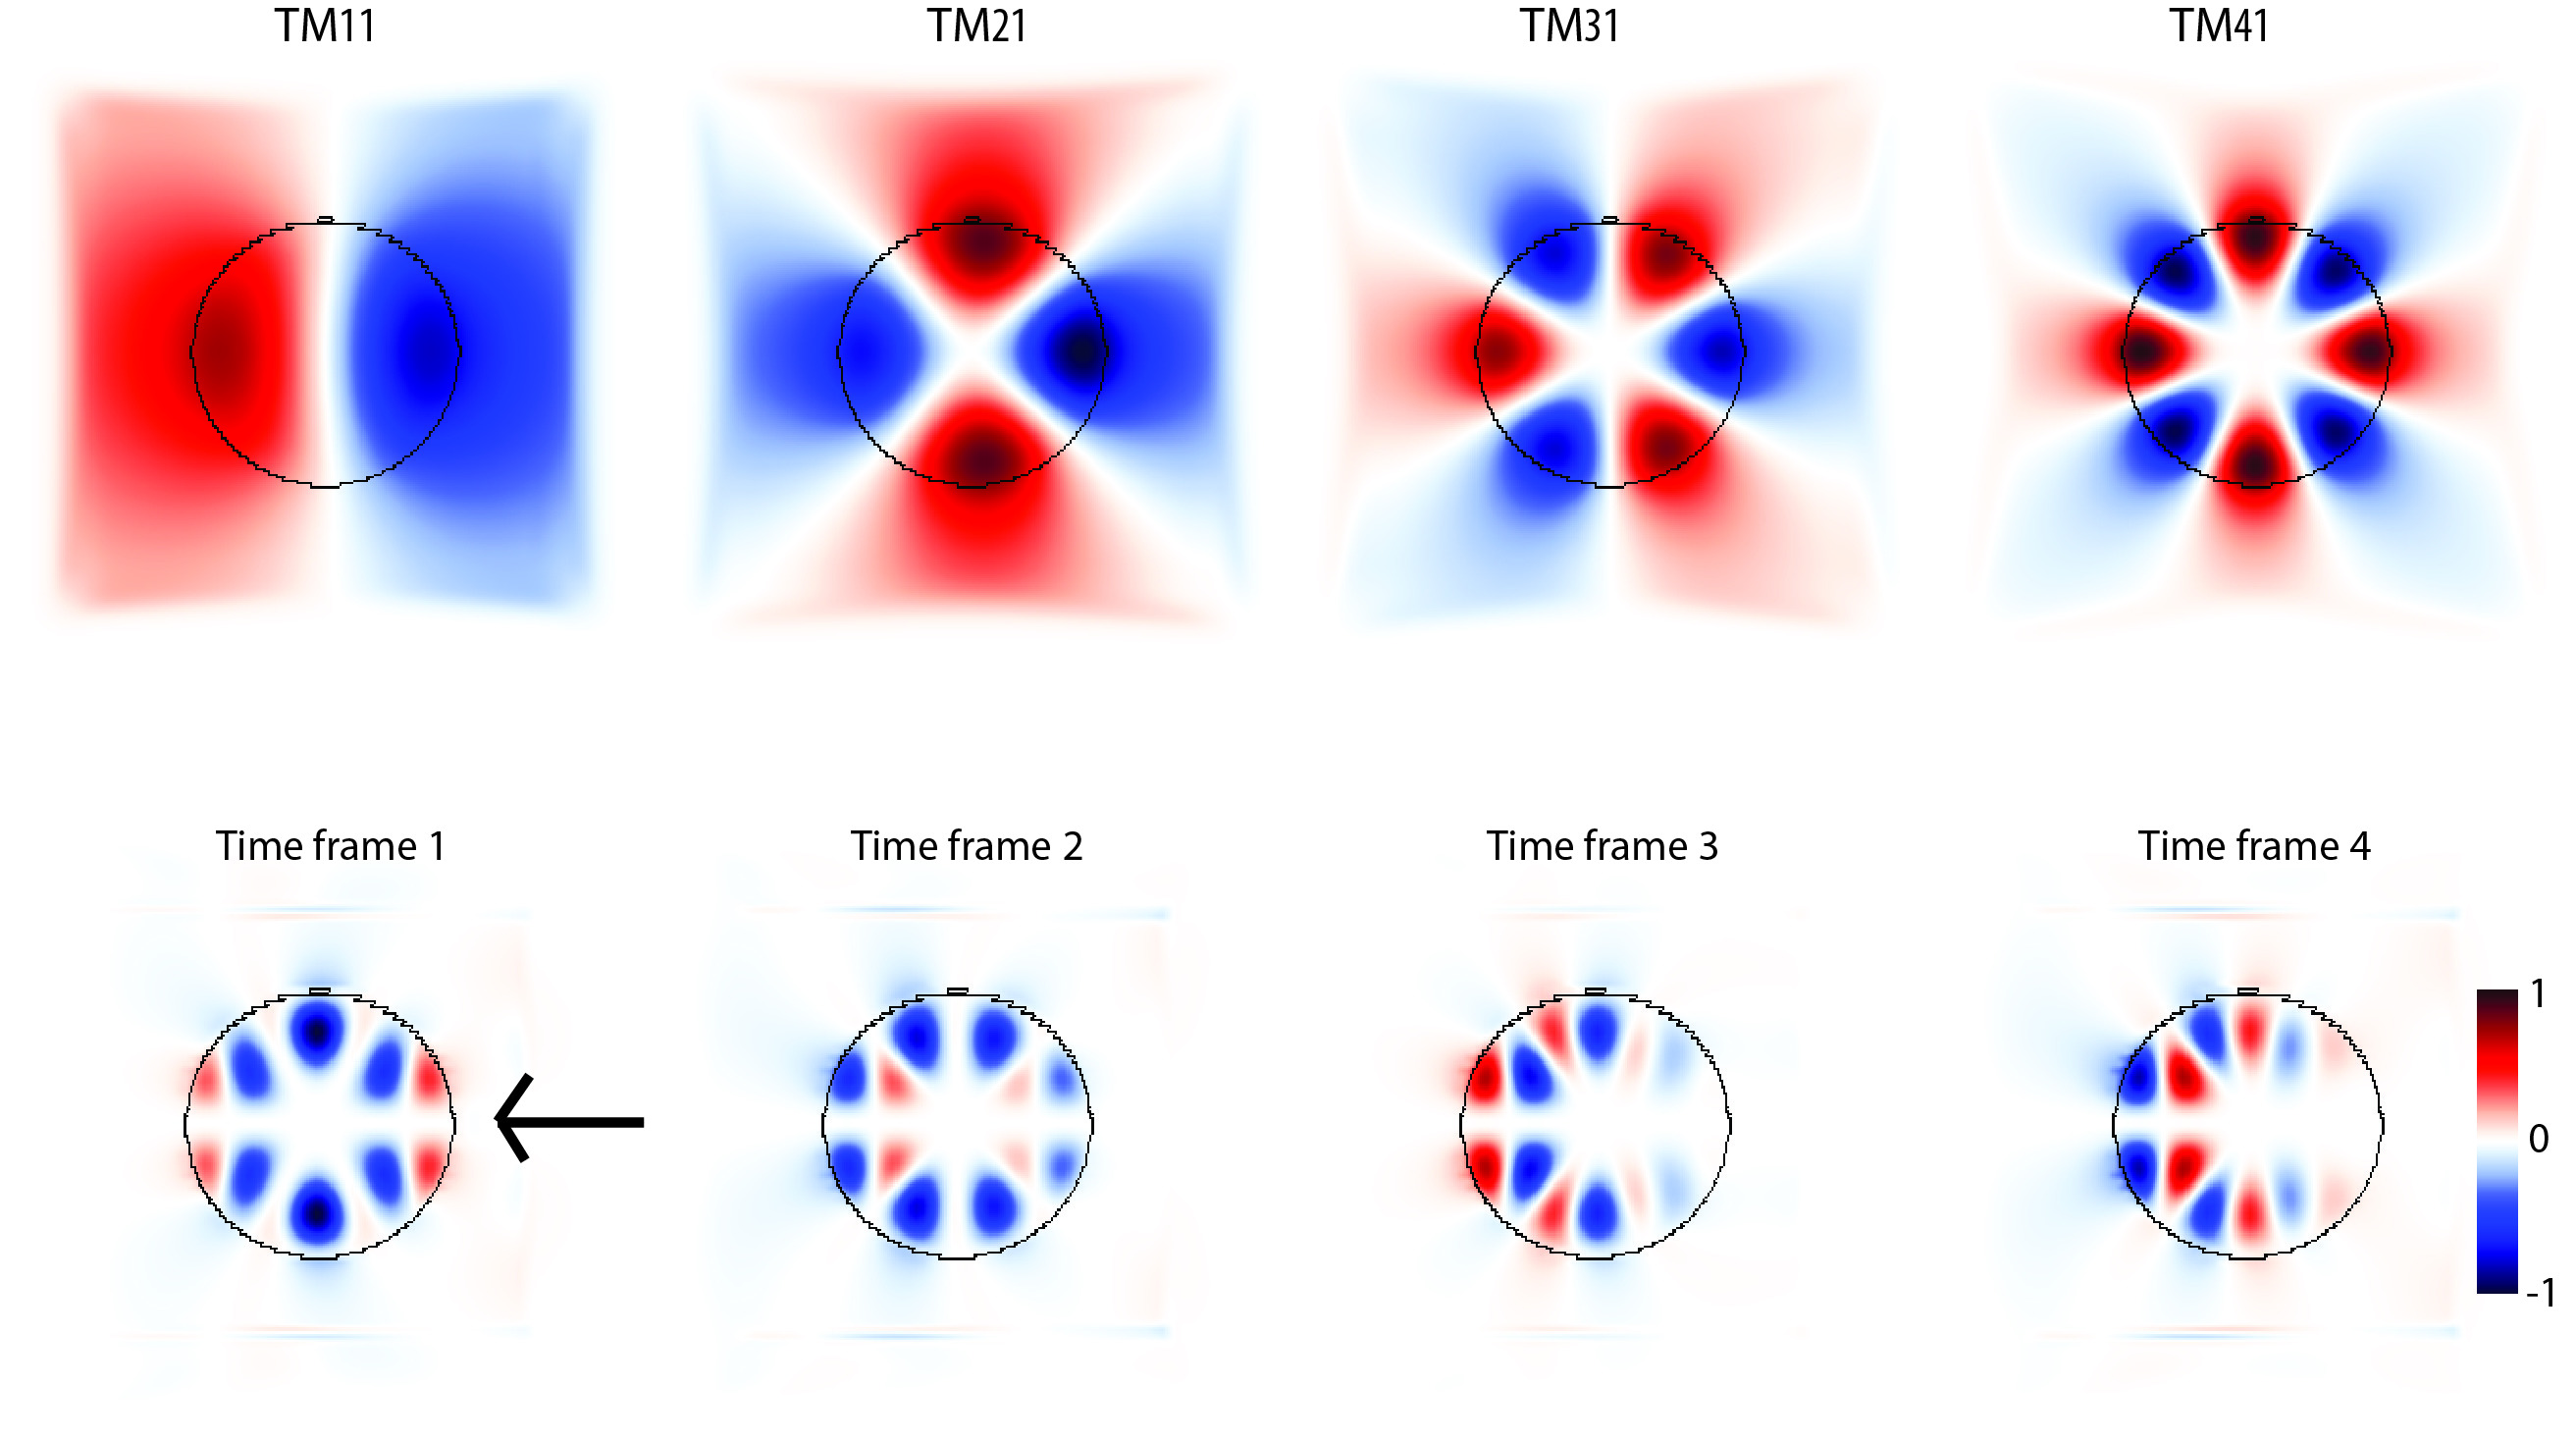
\includegraphics[width=\textwidth]{pictures/LM/CylindEz}
  \label{CylindEz}
\end{figure}

\begin{figure}
  \caption{Simulation Schematic for Cylindrical and Hexagonal Nanowires}
  \centering
  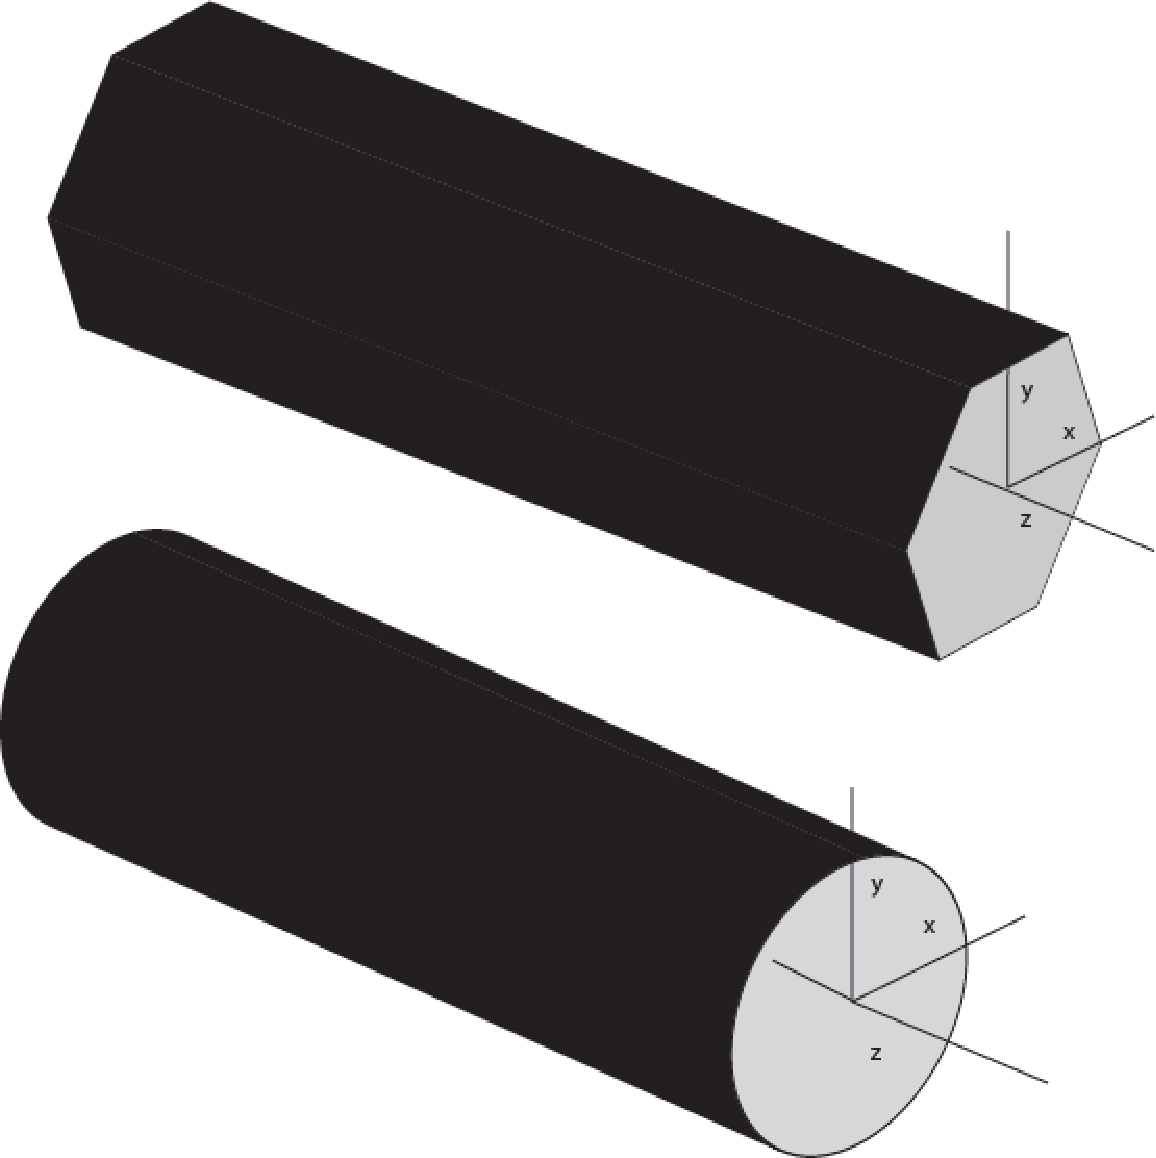
\includegraphics[width=\textwidth]{pictures/LM/NW}
  \label{NW}
\end{figure}

\begin{figure}
  \caption{Geometric Dependence TM radius variation for different Radius and Diameters}
  \centering
  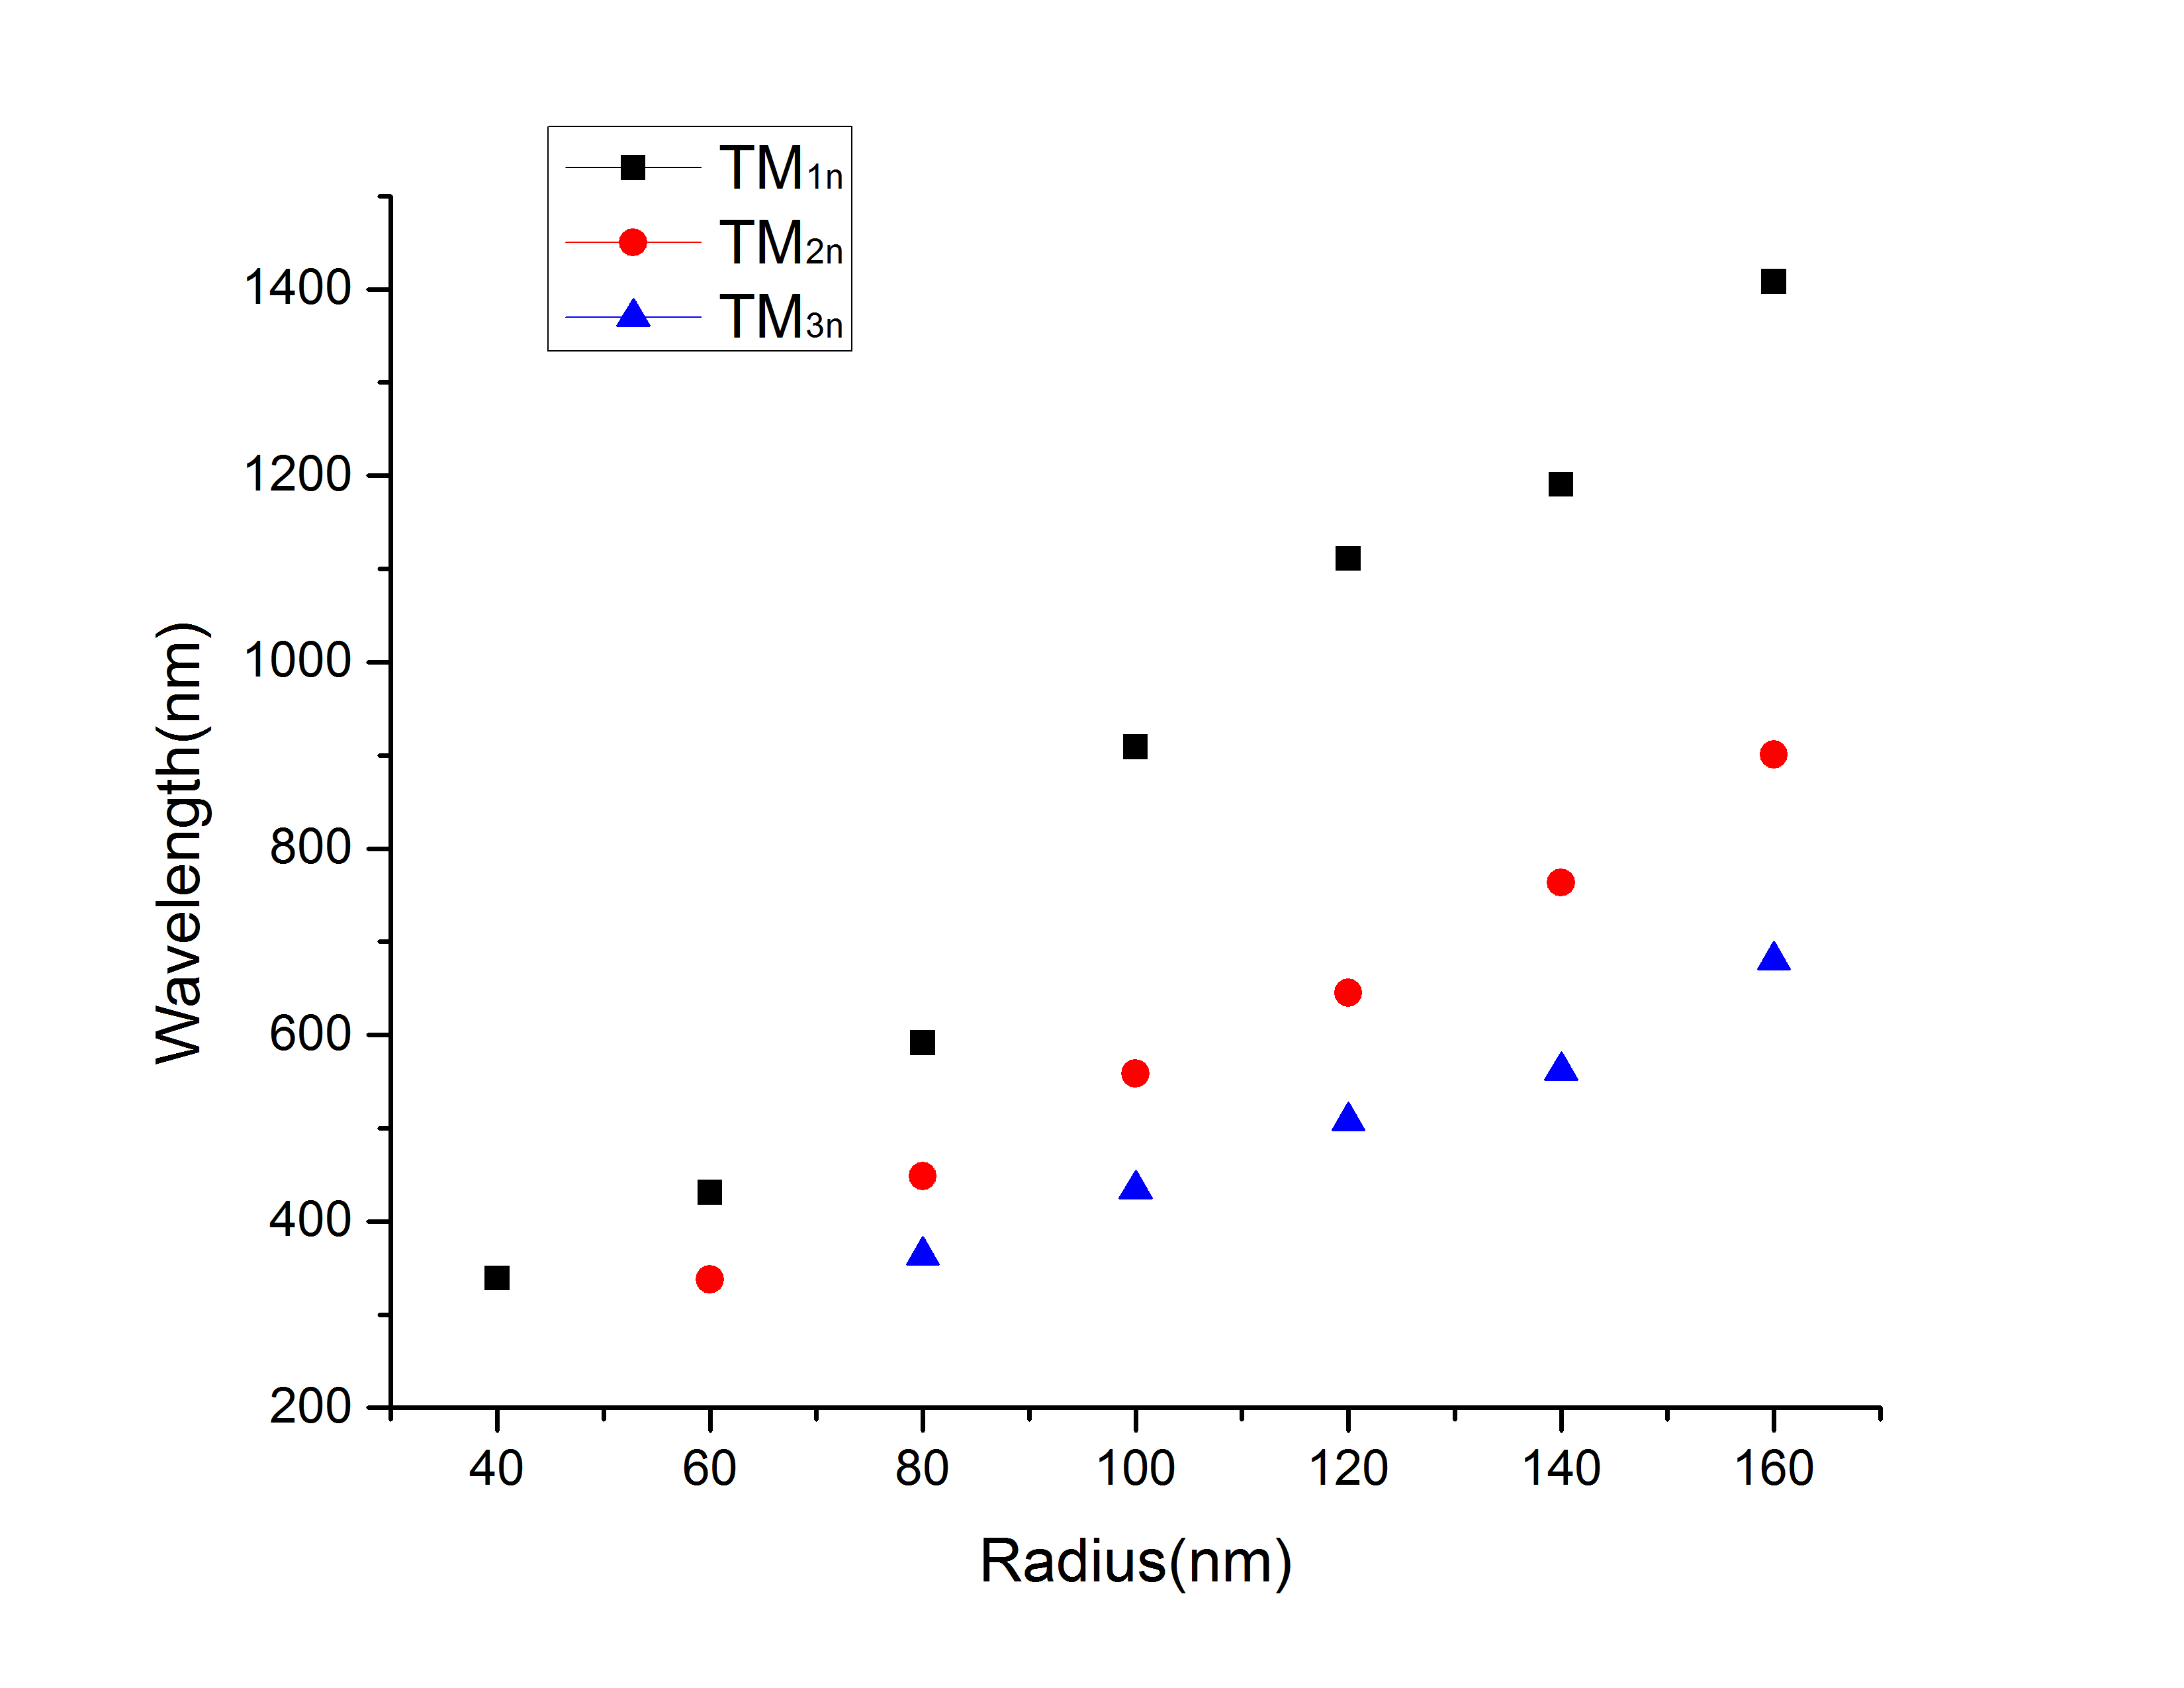
\includegraphics[width=\textwidth]{pictures/LM/TMradius}
  \label{TMradius}
\end{figure}

\begin{figure}
  \caption{Geometric Dependence and Engineering Light with Radius}
  \centering
  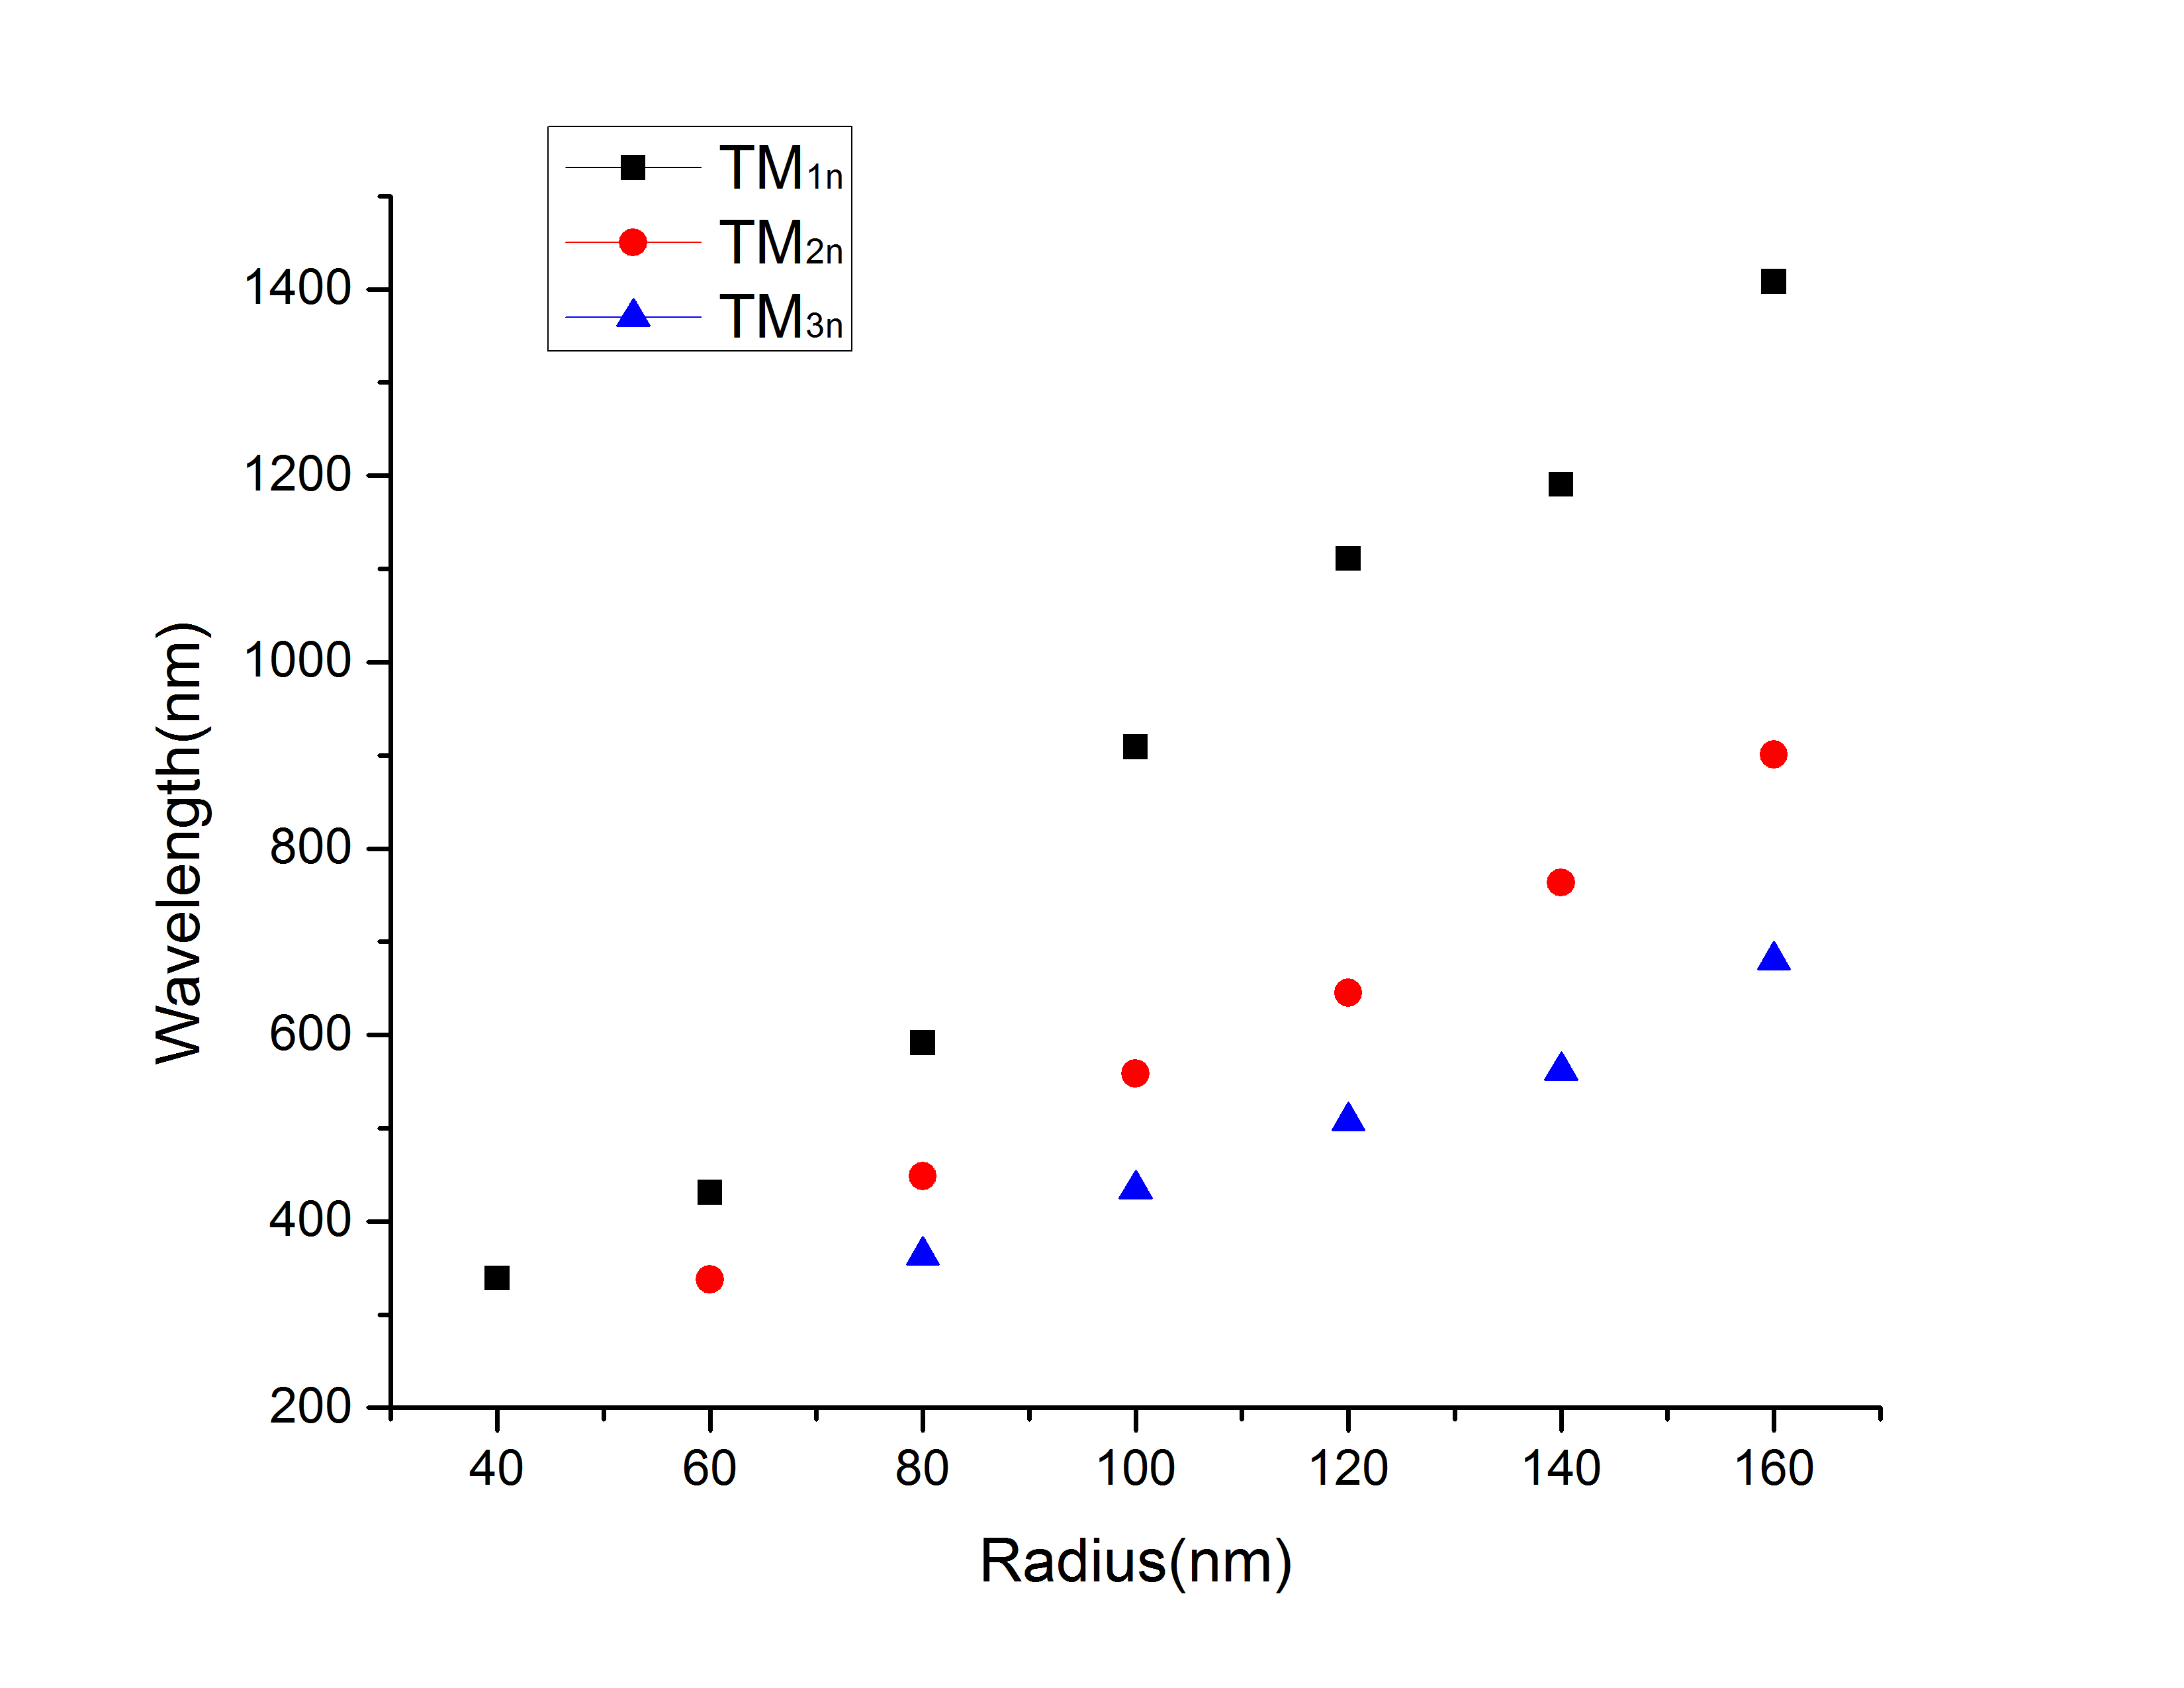
\includegraphics[width=\textwidth]{pictures/LM/TMRadiusScat}
  \label{TMRadiusScat}
\end{figure}

\begin{figure}
  \caption{3D view of Photon Distribution}
  \centering
  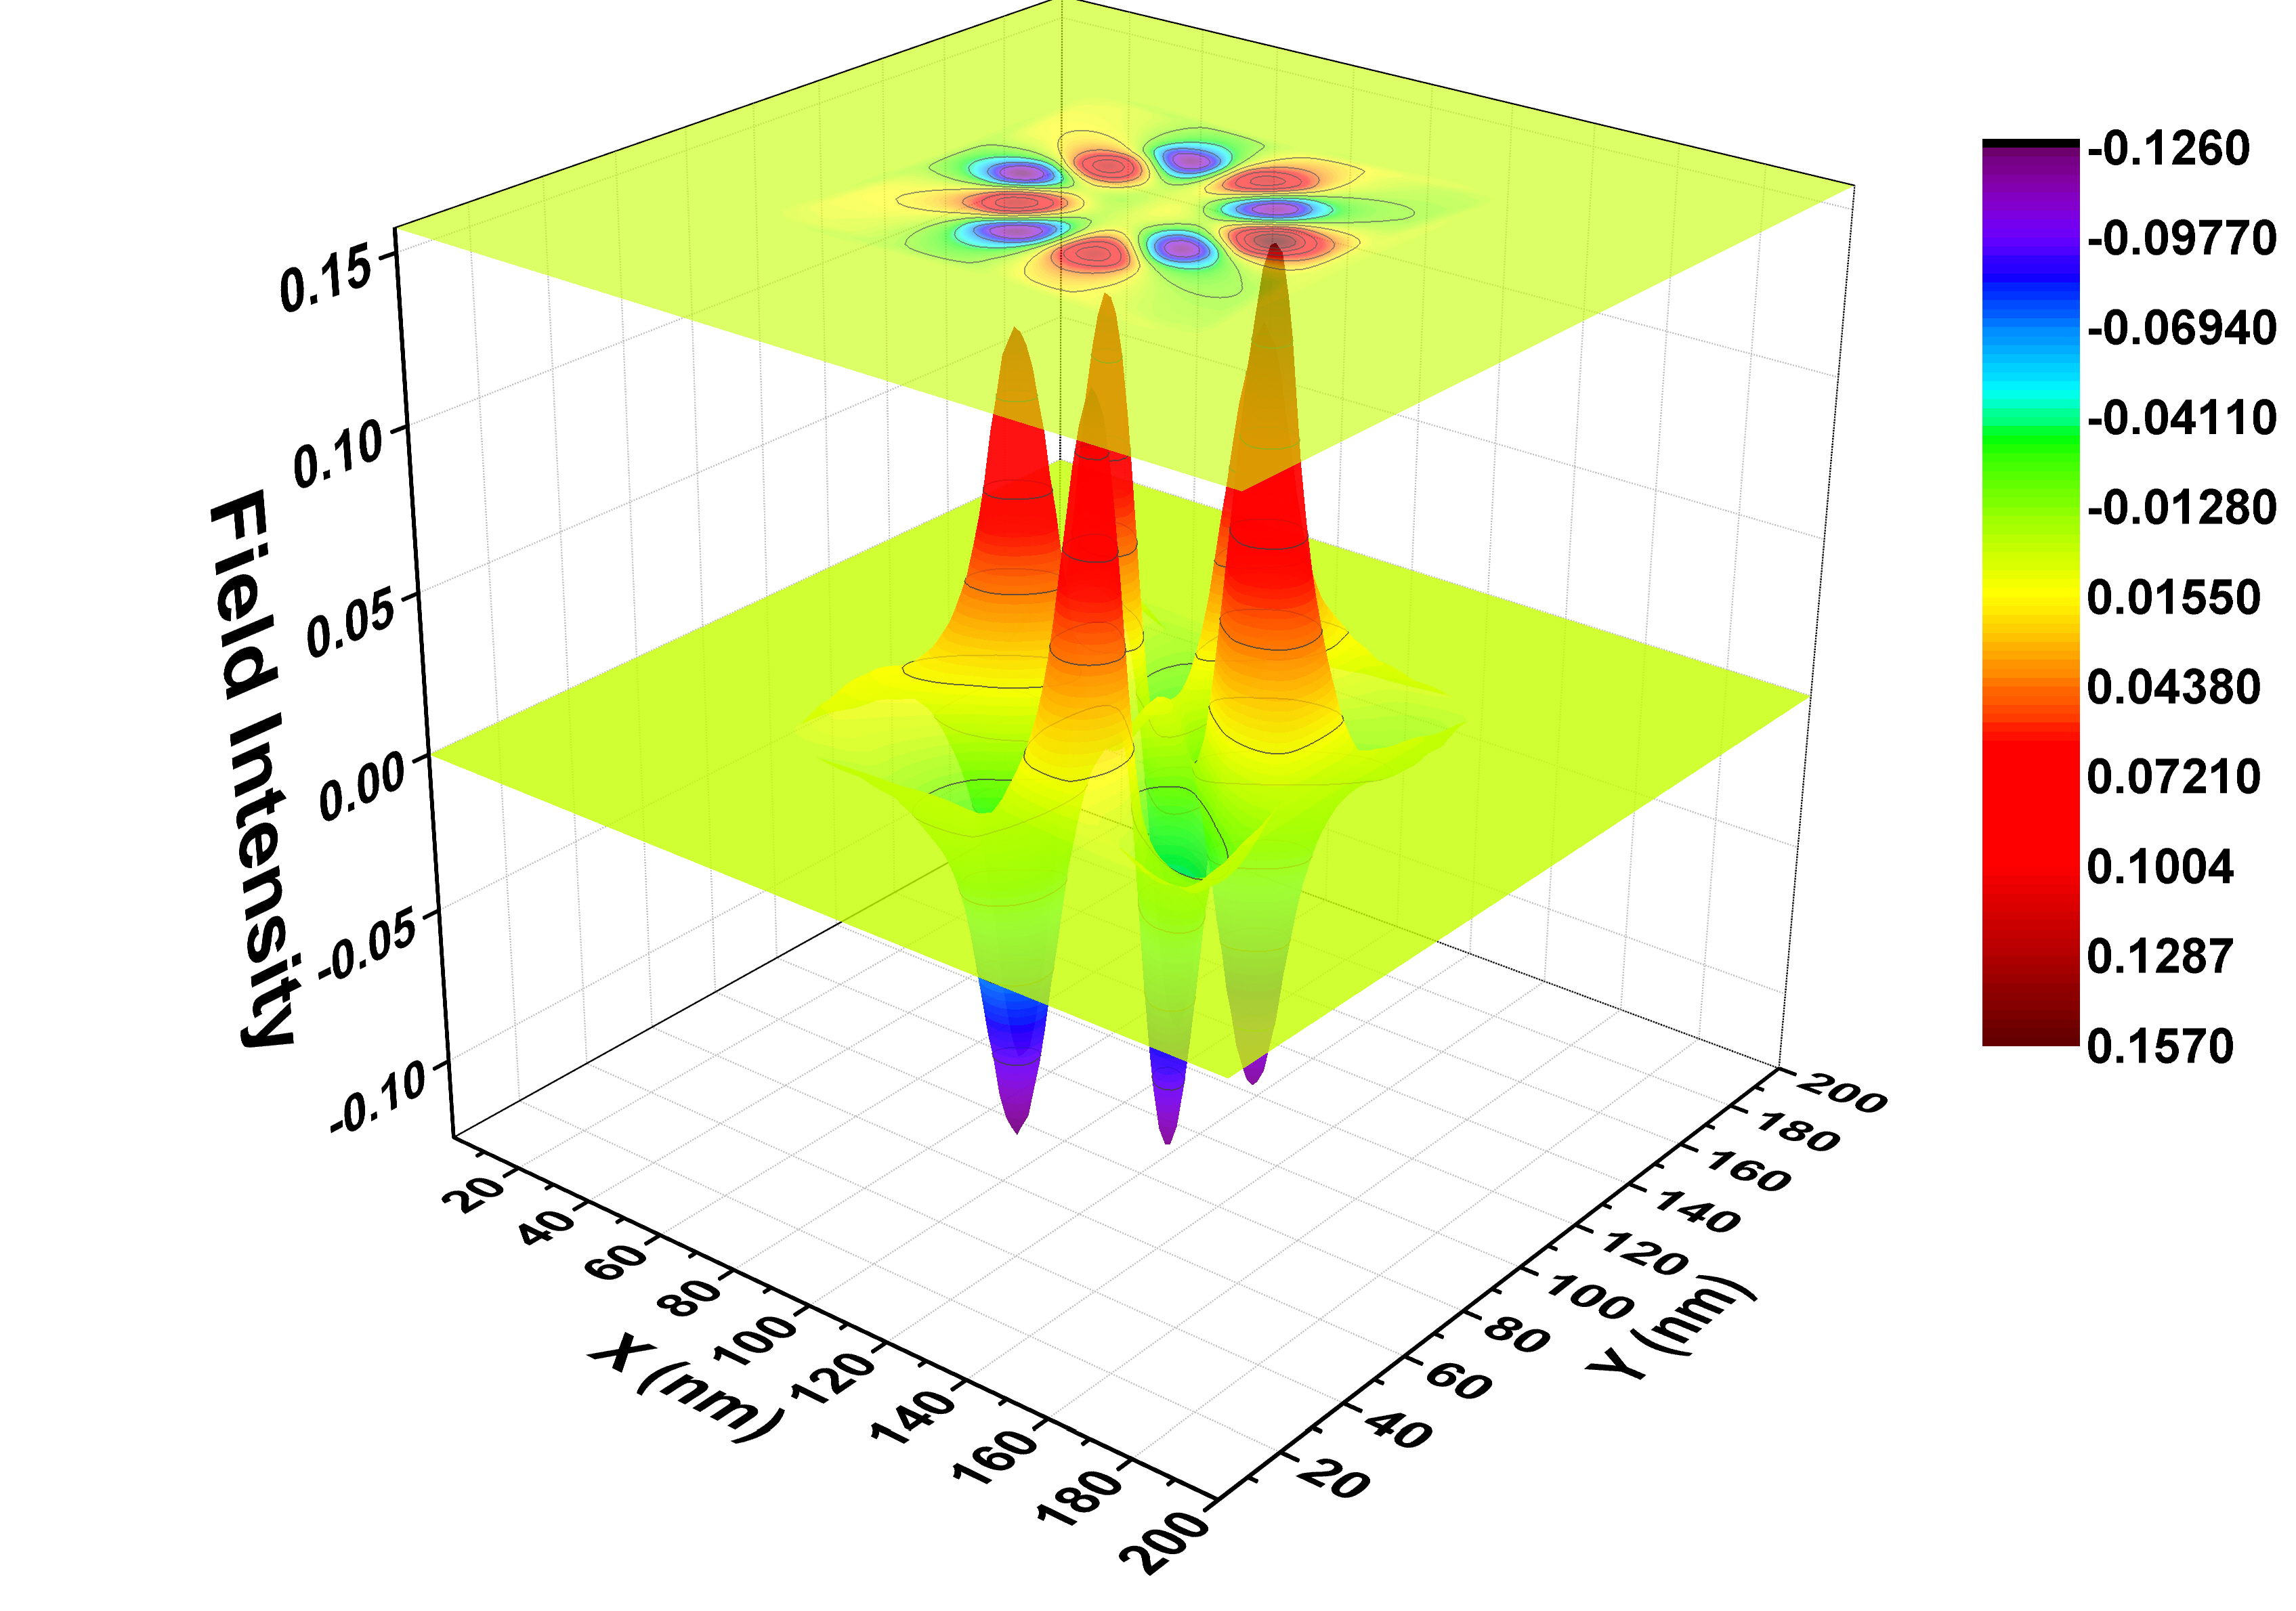
\includegraphics[width=\textwidth]{pictures/LM/photondensity2}
  \label{photondensity2}
\end{figure}
%\subsubsection{\civ-dependent Mean} \label{CIV SED}




  
  %CHAPTER: Electronic Density Distribution
  \suppressfooter{}
  \rightfooter{}
  \chapter{Reduced Electronic Density Distribution} \label{ED}

A heterojuntion is basically a p-n junction in a semiconductor between
materials of different composition. Normal junctions are between p and n type
versions of the same material. But in this case we refer to a juntion formed
betewen two group III-arsenide usually a GaAs/AlAs interface or a GaAs/AlGaAs
interface. Since they are two differnt materials, the band structure is
discontinuous from one material to the other and the band alignment across the
interface is typically of type I, i.e. the band gap of the lower bandgap
material is positioned energetically within the bandgap of the wider bandgap
semiconductor.

Polarization fields 
The usual growth direction for hexagonal III-V materials is
along the polar [0001] axis, for which the crystal lacks inversion symeetry.
This will result in the formation of polarization fields. There are two kinds
of polarization fields. They are spontaneous polarization (SP) and
Piezoelectric polarization (PZ).  The spontaneous polarization exists in polar
semiconductors with a Wurzite or lower symmetry crystal structure and is
related to the deviation of the crystal lattice parameters from the ideal
values for the structure, thereby creating molecular dipoles in the material
building a polarization field just like that formed in ferroelectrics. This
field has a fixed direction along the [0001] c-axis in the Wurtzite lattice.
Therefore the field resulting from spontaneous polarization will point along
the growth direction and this maximizes pontaneous polarization effect in these
systems and renders the problem effectively one-dimensional.

The other type of polarization field, the piezoelectric polarization occurs due
to the presence of strain in the system. When two layers are joined together to
form a heterojunction, the difference in the lattice constant between the two
materials will lead to a strain . This strain also occurs due tot he difference
in the thermal expansion coefficients in the the layers during cool down after
growth. This leads to elastic strain in the layers. 

\section{Self-consistent Schr{\"o}dinger-Poisson Solver} \label{sec:model}

\subsection{Finite Element Method}\label{sec:FEM}

The study of energy band structures of heterostructures needs a detailed
knowledge of optical and transport properties of the heterostructures. These
properties can be found by solving self-consistently Poisson's and
Schr{\"o}dinger's equations for the electron wave functions.


The finite element method (FEM) is a simple and efficient method for solving
ordinary differential equations (ODEs) or partial differential equations (PDSs)
in problem regions with simple boundaries~\cite{bathe2006finite}. FEM can be used to solve for the
Schr{\"o}dinger and Poisson equation self-consistently. A generic formulation for a PDE with the following form: 

\begin{equation}
  |D|u(x) = f(x)\in\Omega
  \label{eq:generic}
\end{equation}

where $D$ is an arbitrary operator, and $\Omega$ defines the geometry. In order
to solve this PDE using FEM, eq.~\ref{eq:generic} has to be rewritten in weak
variational form with the boudary conditions:

\begin{eqnarray}
\begin{aligned}
  \left\{
    \begin{array}{ll} 
      u(x) = u_{0}(x) \qquad on \quad \Gamma_D   \\
      \frac{\partial{u}}{\partial{n}} = g_0(x) \qquad on \quad \Gamma_N
    \end{array}
  \right.
\end{aligned}
\label{eq:generic_BC}
\end{eqnarray}

where $\Gamma_D$ and $\Gamma_N$ signifies Dirichlet and Neumann boundary
condition. By introducing an arbitrary function $v$ and multiplying the PDF
with $v$, then integrating over all the domain $\Gamma$ and separating every
second-order derivative using integration by parts, the original PDE can be
carried out in the weak form as:

\begin{equation}
  \int_{\Omega}|D^\prime|(u{\cdot}v)\ d\Omega + \\
  \int_{\Gamma_N}gv\ \partial\Omega = \\
  \int_{\Omega}fv\ d\Omega \quad \forall v \in \hat{V}\\
  \label{eq:weakPDE}
\end{equation}

where $D^\prime$ is the reduced operator after performing integration by part to the second-order derivatives, and $\hat{V}$ is the function space where an arbitrary function $v$ belongs to. The function $u$ lies in V, which could be different than $\hat{V}$. This continuous variational problem need to be reformulated to discrete problem with discrete space $\hat{V}_d \subset \hat{V}$ and $V\subset{V}$ so that the boundary conditions can be restated as:

\begin{equation}
  \int_{\Omega}|D^\prime|(u_d{\cdot}v)\ d\Omega + \\
  \int_{\Gamma_N}gv\ \partial\Omega = \\
  \int_{\Omega}fv\ d\Omega \quad \forall v \in \hat{V}_d\subset \hat{V}\\
  \label{eq:weakPDE_BC}
\end{equation}

It is more convenient to use unified notation for linear weak forms $a(u,v) =
L(v)$ with $a(u,v)=\int_{\Omega}|D^\prime|(u_d{\cdot}v)\ d\Omega$ and
$L(v)=\int_{\Omega}fv\ d\Omega- \int_{\Gamma_N}gv\partial\Omega$.

\subsection{Variational form of Schr{\"o}dinger and Poisson equations}\label{sec:VF}

A general Poisson equation for electrostatics is giving by~\cite{tan1990self}:

\begin{equation}
  \frac{d}{dx}(\epsilon_s(x)\frac{d}{dx})\Phi(x)=\frac{-q[N_D(x)-n(x)]}{\epsilon_0}
  \label{eq:Poisson}
\end{equation}

where $\epsilon_s$ is the dielectric constant of the material, $N_D$ is the
ionized donor concentration, $\Phi$ is electrostatic potential, and $n$ is the
electron density. Since Eq.~\ref{eq:Poisson} only has a piecewise dielectric
constant, the domain can be divided into subdomains by different dielectric
constants. The Poisson equation can be rewritten as:

\begin{equation}
  \epsilon_s\nabla^2\Phi(x)=\frac{-q[N_D(x)-n(x)]}{\epsilon_0}
  \label{eq:Poisson_VF}
\end{equation}

Note that the operator $|D|$ is replaced by $\nabla^2$, and the source term
$f(x)$ is replaced with the scaled difference of the ionized donor
concentration and the electron density. Then the Poisson equation can be
reformulate to the weak variational form following the previous procedures.

\begin{equation}
  \int_\Omega\epsilon_s\epsilon_0\nabla\Phi\nabla{v}\ d\Omega = \\
  \int_{\Omega}[{-q[N_D(x)-n(x)]}]{v(x)}\ d\Omega
  \label{eq:Poisson_VFF}
\end{equation}

The weak variational form of Schr{\"o}dinger's equation can be derived from the general differential form following by the similar manner:

\begin{equation}
  -\frac{\hbar^2}{2}\frac{d}{dx}(\frac{1}{m^\ast(x)}\frac{d}{dx})\psi(x)+\\
  V(x)\psi(x)=E\psi(x)
  \label{eq:Schrodinger}
\end{equation}

where $m^\ast(x)$ is the effective mass. Equation~\ref{eq:Schrodinger} can
rewritten after taking the effective mass out, as it will remain constant in a
single region.

\begin{equation}
  \frac{\hbar^2}{2{m^\ast}}\nabla^2\psi(x)+[E-V(x)]\psi(x) = 0
  \label{eq:Schrodinger_VF}
\end{equation}

Multiply both sides by a test function $v$, which is arbitrary with the condition that it vanishes on the boundaries of the system.

\begin{equation}
  \int_\Omega\frac{\hbar^2}{2{m^\ast}}\frac{\psi}{x}\frac{v}{x}\ d\Omega +\\
  \int_{\Omega}V(x)\psi(x)v(x) = \int_{\Omega}E\psi(x)v(x)\ d\Omega 
  \label{eq:Schrodinger_VFF}
\end{equation}

\subsection{Numerical Implementation}\label{sec:NI}

To obtain the electronic properties, the electrostatic potential
$V(x=-q\phi(x)+{\triangle}{E_c}(x)$ first sets to zero. Then the envelope
functions and the eigen energies are calculated according to the Schr{\"o}dinger
equation~\ref{eq:Schrodinger}. A Poisson equation~\ref{eq:Poisson} is solved
after the determination of the quasi Fermi level $E_F$ by solving charge
neutrality equation. The electron concentration can now be calculated based on:

\begin{equation}
  n(x) = {\sum\limits_{k=1}^{m}}{\psi^\ast}_k(x){\psi_k}(x){n_k}
  \label{eq:EC}
\end{equation}

\begin{equation}
  n_k = \frac{m&^\ast}{\pi\hbar^2}{\int\limits_{E_k}^{\infty}}\frac{1}{1+e^{(E-E_F)/KT}}dE
  \label{eq:EO}
\end{equation}

where $\triangle{E_c(x)}$ is the pseudopotential energy due to the band offset
at the heterointerface, $n_k$ is the electron occupation number which can be
calculated by Fermi-Dirac distribution function with Fermi level $E_F$,
$\psi_k$ is the wavefunction in the $k^{th}$ state, and $E_k$ is the eigen
energy in state k. Finally, a check of the electrostatic potential update
decides whether the iteration terminates. The procedure of this
Schr{\"o}dinger-Poisson solver has been demonstrated in the flow chart diagram
as in Fig.~\ref{SchrodingerPoissonSolver}.

Implementing the FEM method when solving the Schr{\"o}dinger and Poisson
equations requires the construction of a mesh defining local coordinate
surfaces. For each node of this mesh, the unknown eigen functions and eigen
values are found, replacing the original differential equations by variational
forms. In order to make the FEM method more effective, implementing a small
mesh when the wavefunction is changing rapidly and a large mesh during a slow
change in the wavefunction is necessary.

\begin{figure}
  \caption{A flow chart diagram of the Schr{\"o}dinger-Poisson solver. The procedure is only discussed for electrons in the conduction band for simplicity but it also hold true for holes in the valence band using analogous formulas.}
  \centering
  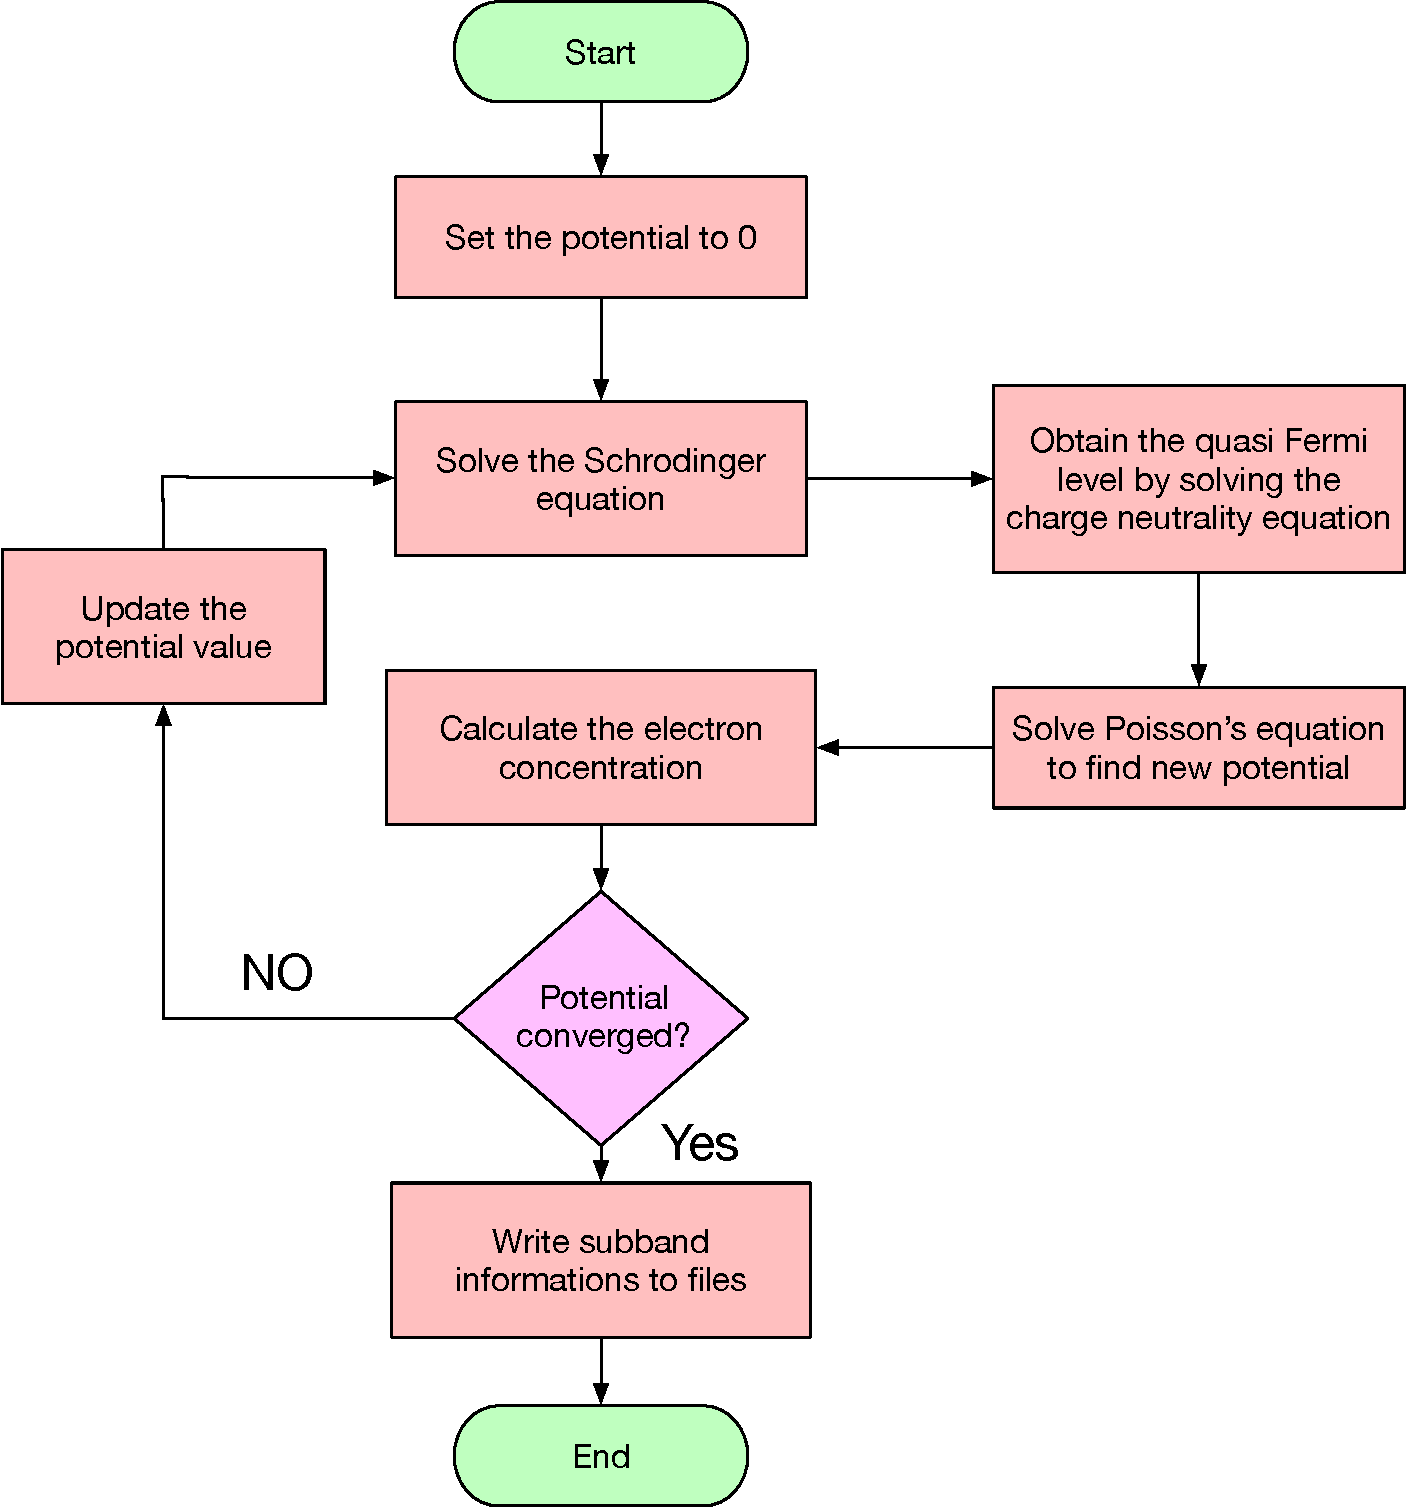
\includegraphics[width=\textwidth]{pictures/ED/SchrodingerPoissonSolver}
  \label{SchrodingerPoissonSolver}
\end{figure}

\section{Electronic Distribution in Nanowires} \label{sec:spectra}

The electronic band structure and the electronic density of cylindrical and
hexagonal GaAs/AlGaAs core-shell nanowire are calculated self-consistently by
solving Poisson and Schr{\"o}dinger equations
\cite{wong2011nanoscale,bertoni2011electron} using $\bf{nextnano^3}$ simulation
packages \cite{birner2007nextnano}, which is a commercial computer aid software
with better physical method for the calculation of the quantum mechanical
properties of an arbitrary combination of geometries and materials.

\subsection{Cylindrical Core-Shell Nanowire}

The cylindrical core-shell nanowire has been investigated with a radius of 20nm
GaAs core and 15nm AlGaAs shell. An additional Si-doped AlGaAs layer with a
0.33 mole fraction is placed between the core and shell. The thickness of this
layers is 5 nm. The left part of Fig.~\ref{CylindricalCSNW} shows the electron
density distribution in 3D view. A free-electron gas is formed in the GaAs core
and at the inner heterointerface with a small fluctuation of density along the
interface. There is a very small amount of electron gas distributed at the
center of the core. Further simulation with different doping density $\rho_D$
shows similar distribution of the electron gas but very small variation of the
magnitude of the intensity. On the right part of Fig.~\ref{CylindricalCSNW},
the black line represents the conduction and valence band bending and the blue
line shows the electron density along the vertical cut of this cylindrical
CSNW.

\begin{figure}
  \caption{(left) Electron charge distribution in 3D illustration. (right) Conduction and valence band bending (black lines) and electron density distribution (blue line) for cylindrical core-shell nanowire. The inset shows the data captured from a vertical slice of the simulated structure.}
  \centering
  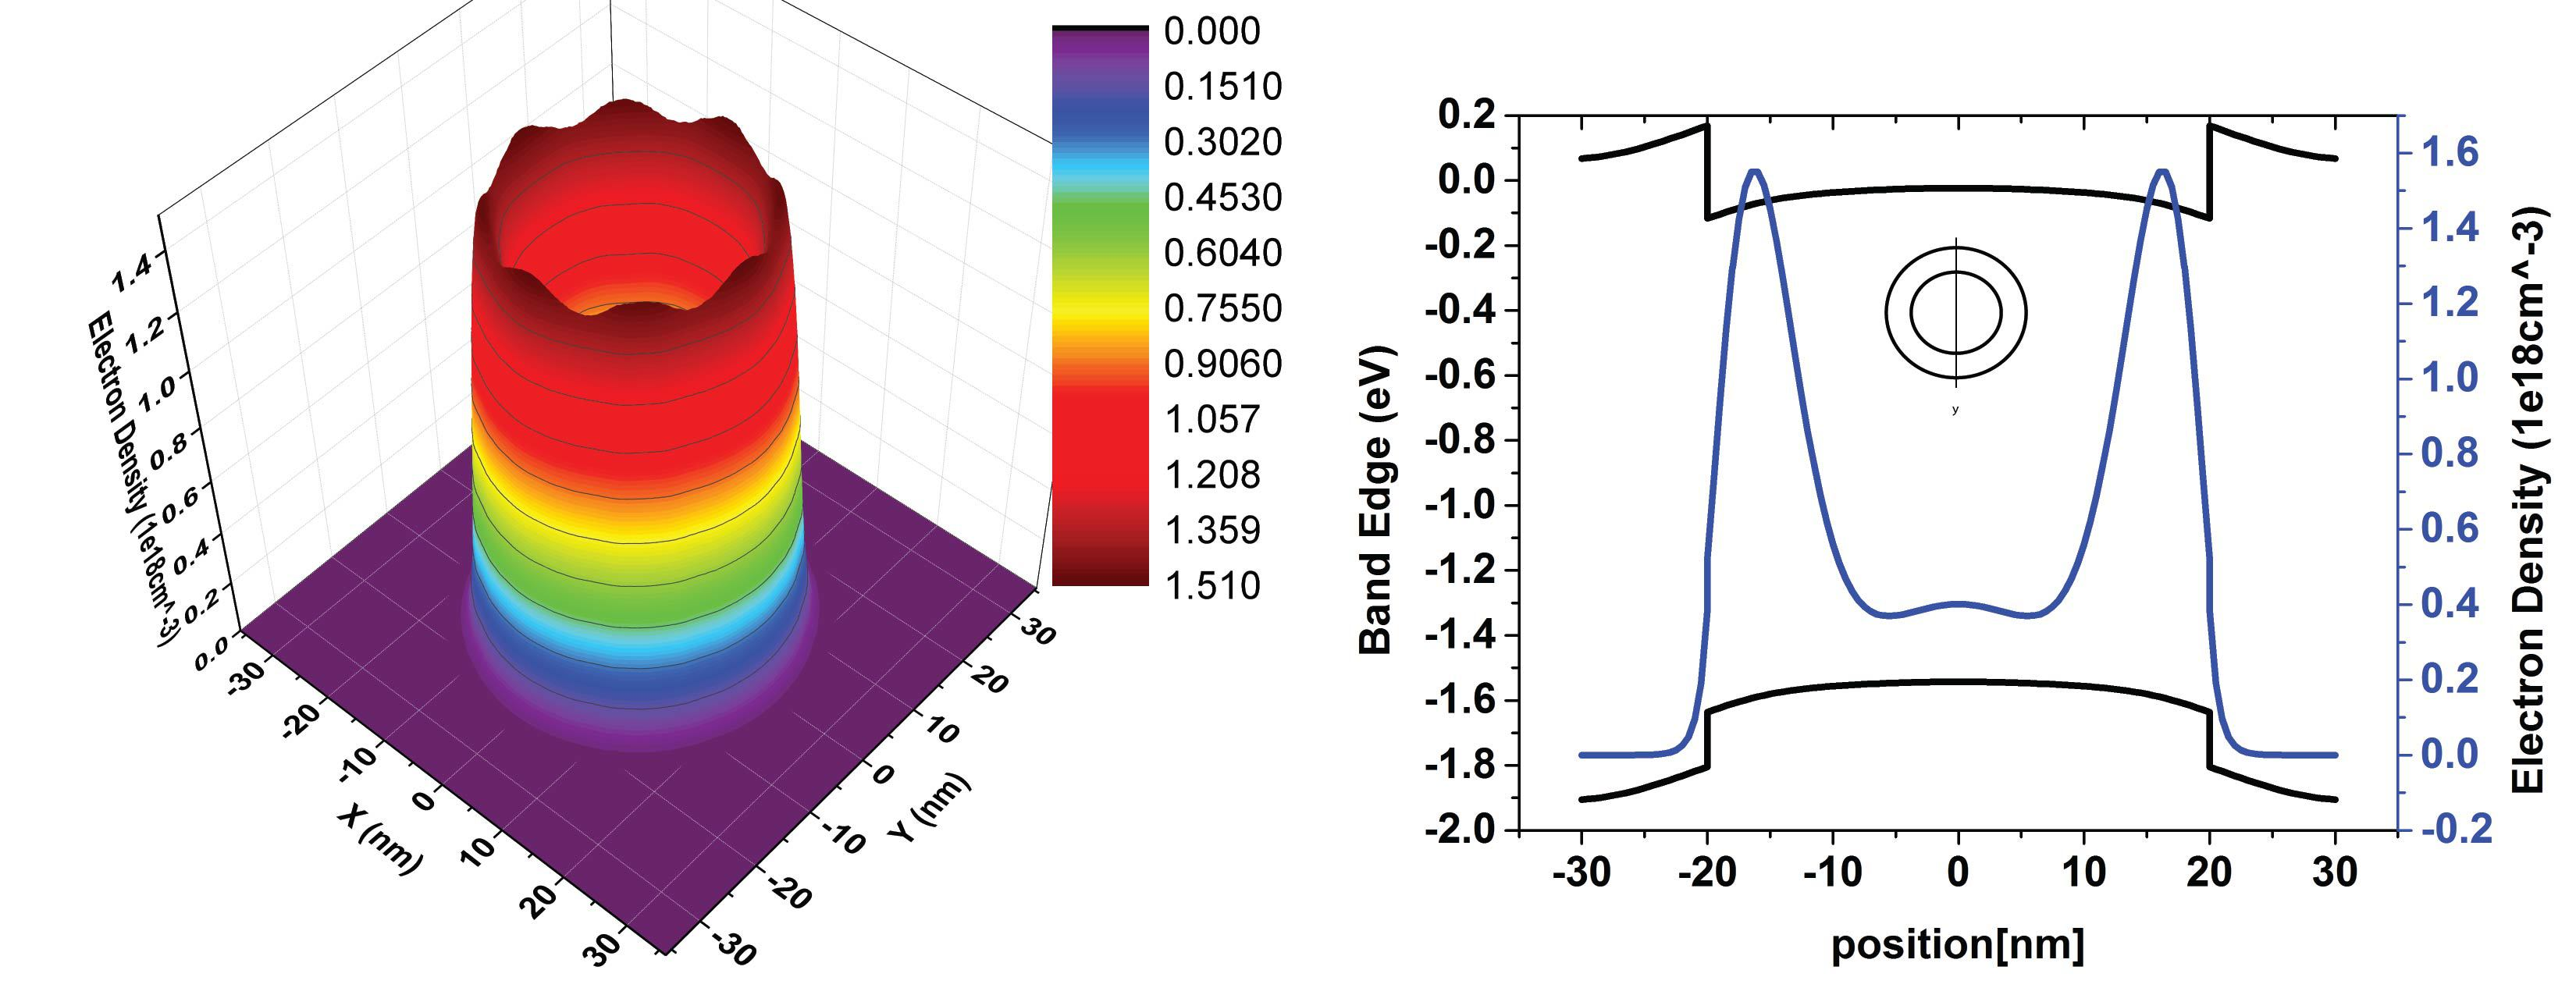
\includegraphics[width=\textwidth]{pictures/ED/CylindricalCSNW}
  \label{CylindricalCSNW}
\end{figure}

\subsection{Hexagonal Core-shell Nanowire} \label{sec:indv_lines}

Due to the hetero-interface between the core and shell and the piezoelectric
force at the corners, the electronic states distribution inside of the
hexagonal core-shell nanowire is not always three-dimensional case or
two-dimensional like in cylindrical NWs. Lower-dimensional electron gas arises
with increased doping density. A delta-doped hexagonal CSNW heterostructure has
been simulated. The radius of GaAs core and AlGaAs shell is 43.3 nm and 45 nm,
respectively, with a 17.3 nm AlGaAs spacer in between. The thickness of
Si-doped AlGaAs is 1.6 nm with a 0.33 mole fraction of AlGaAs. This Si-doped
AlGaAs layer is used to populate a (triangular) quantum well at the
heterointerfaces. Such a well can also be produced by sandwiching a GaAs layer
radially between two wider bandgap materials. 

The left part of Fig.~\ref{3DCharge}, \ref{2DCharge} and \ref{1DCharge} shows
the spatial distribution of the free-electron gas for the three values of the
doping density indicated as (Fig.~\ref{3DCharge}) $\rho_D = 9.2 \times 10^{18}
cm^{-3}$, (Fig.~\ref{2DCharge}) $\rho_D = 9.6 \times 10^{18} cm^{-3}$,
(Fig.~\ref{3DCharge}) $\rho_D = 1.5 \times 10^{19} cm^{-3}$. On the right part,
the electronic band structure (blue line) and the electronic density (red line)
of hexagonal GaAs/AlGaAs core-shell nanowire are depicted for vertical slice
(top, right) or horizontal slice (bottom, right).

At the lowest doping, shown in Fig.~\ref{3DCharge}, the charge is distributed
deep into the core. The distribution is only slightly modulated (right panels)
crossing the core along either the y cross section or x cross section, and
slightly depleted in the center of the core.

\begin{figure}
  \caption{(left) Three dimensional electron charge distribution in 3D illustration. (right) Conduction and valence band bending (blue lines) and electron density distribution (red line) for hexagonal core-shell nanowire with a low doping density. The inset shows the data captured from a (top) vertical or (bottom) horizontal slice of the simulated structure.}
  \centering
  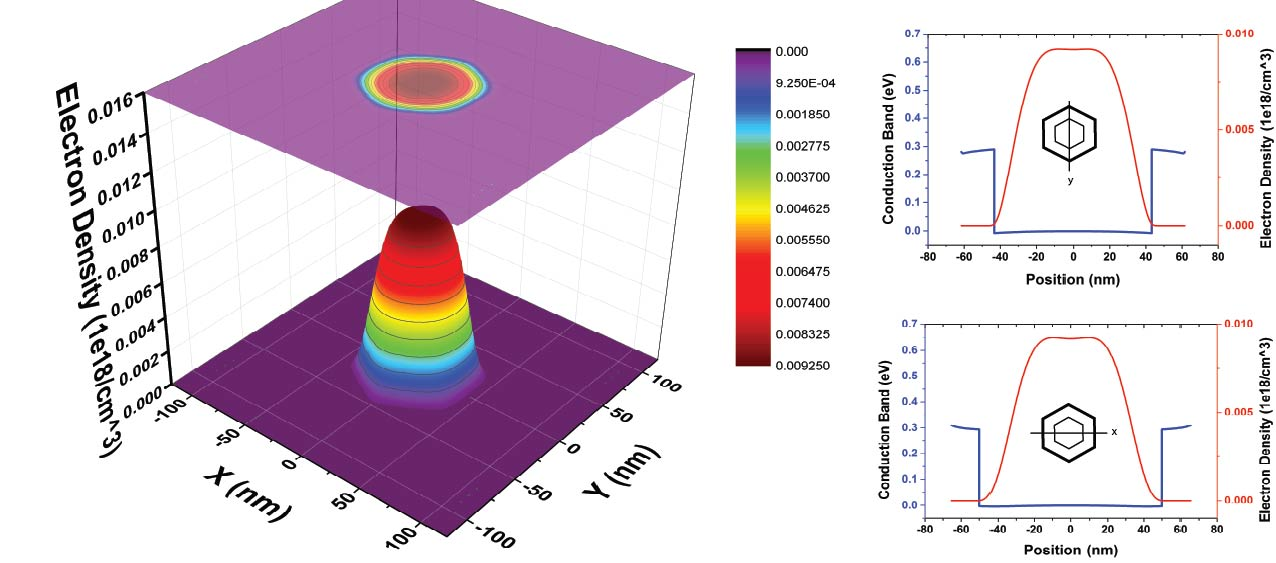
\includegraphics[width=\textwidth]{pictures/ED/3DCharge}
  \label{3DCharge}
\end{figure}

As the doping is increased in Fig.~\ref{2DCharge}, the charge depletion in the
center is more pronounced, and the charge moves toward the heterojunction
interface, leaving this "volcano" like charge distribution in the left part of
Fig.~\ref{2DCharge}. The two-dimensional electron gases (2DEG) are formed at the
heterointerface of GaAs core and AlGaAs shell.

\begin{figure}
  \caption{(left) Two dimensional electron charge distribution in 3D illustration. (right) Conduction and valence band bending (blue lines) and electron density distribution (red line) for hexagonal core-shell nanowire with a moderate doping density. The inset shows the data captured from a (top) vertical or (bottom) horizontal slice of the simulated structure.}
  \centering
  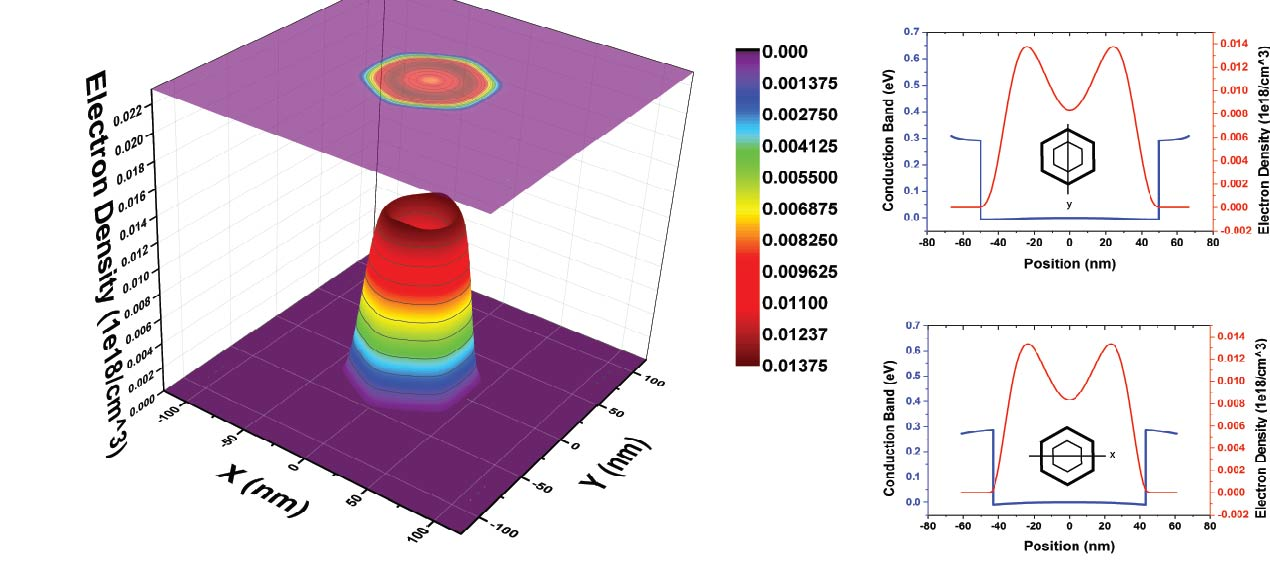
\includegraphics[width=\textwidth]{pictures/ED/2DCharge}
  \label{2DCharge}
\end{figure}

As the doping is further increased in Fig.~\ref{1DCharge}, the shell 2DEG form
at the six (6) core-shell hetero-interface facets, with six (6) pillars of
one-dimensional electron gas (1DEG) forming at the 6 vortices. In addition, as
shown in the right part of the Fig.~\ref{3DCharge}, \ref{2DCharge} and
\ref{1DCharge}, the electronic density of Fig.~\ref{1DCharge} is around two
orders of magnitude higher than 2DEG and bulk counterparts. The results also
matched the other groups' simulation results very well~\cite{Wong:2011tn,
Bertoni:2011hn}.


\begin{figure}
  \caption{(left) One dimensional electron charge distribution in 3D illustration. (right) Conduction and valence band bending (blue lines) and electron density distribution (red line) for hexagonal core-shell nanowire with a high doping density. The inset shows the data captured from a (top) vertical or (bottom) horizontal slice of the simulated structure.}
  \centering
  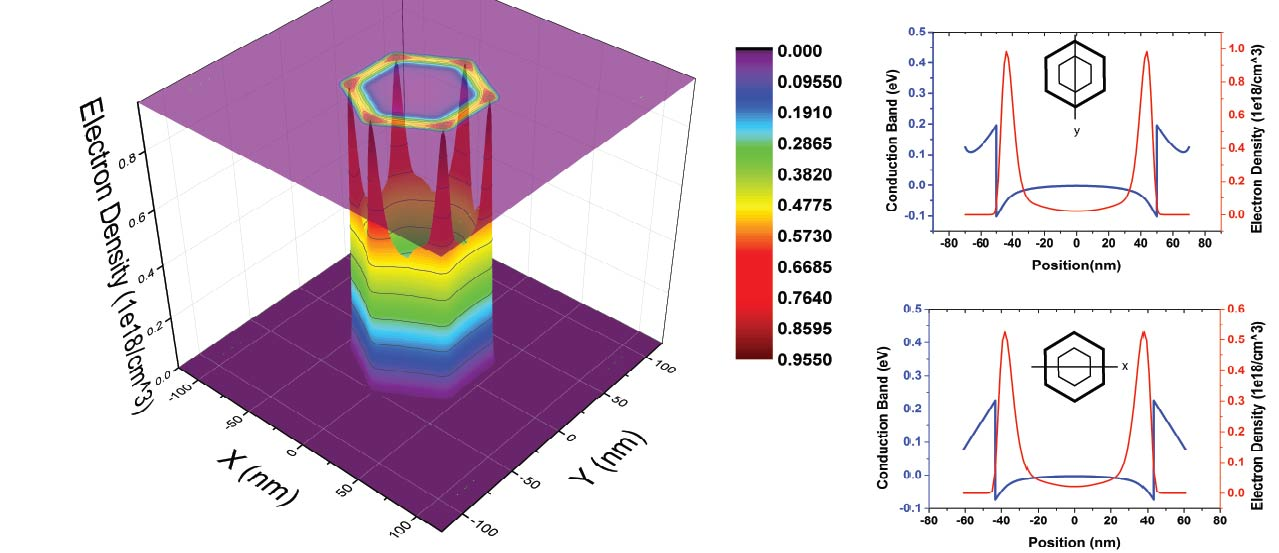
\includegraphics[width=\textwidth]{pictures/ED/1DCharge}
  \label{1DCharge}
\end{figure}


\section{Conclusions} \label{sec:conclusions}

In this chapter, the finite-element-method implemented self-consistent
Shr{\"o}dinger-Poisson solver has been discussed. In addition, a cylindrical
and hexagonal core-shell nanowire structure has been simulated and compared
with different doping density. The simulated results show unique electron
density distribution in hexagonal CSNW with large doping density. This unique
distribution of electrons has also been verified experimentally by electron
holographic tomography~\cite{Wolf:2011if} 


  %CHAPTER: Rate Management
  \suppressfooter{}
  \restorefooter{}
  \chapter{Dimensional Dependence of Optical Transition Rates} \label{RM}
 
\section{Time-dependent Perturbation Theory} \label{dust_seds}

%\subsection{} \label{dust_corrections}

%\subsection{A Uniform Sample}
%\subsection{\ltwofive\ and \bctwofive\ Distributions} \label{l_bc_dust}
%\subsection{Extinction Corrected SEDs} \label{l_bc_dust}

\section{Upward and Downward Transition Rates} \label{mbh_seds}

\section{Contributing Factors} \label{BH_conclusions}
\subsection{Overlap Integral}
\subsection{Oscillator Strength}
\subsection{Joint Optical Density of States}


  %CHAPTER: Laser Threshold Calculation
  \chapter{Modeling Lasing Threshold} \label{LT}


\section{History of Semiconductor Lasers} \label{corrections} As we know,
semiconductor lasers are important optoelectric devices ofr optical
communication systems. They are essential components for building optical
communication systems. There are intensive research results and achievements
from beginning.  In 1917, Einstein predicted the existence of spontaneous and
stimulated emission by which an atom can emit radiation. The first
semiconductor lasers were fabricated in 1962 using homojuncations. These lasers
had high threshold current density ( 19000/A/cm2 ) and operated at cryogenic
temperatures.  The concept of heterojuntion semiconductor lasers was realized
in 1969~1970 with a low threshold current density (1600 A/cm2) operating at
room temperature. These double-heterostructure diode lasers provide both
carrier and optical confinements, which imporve the efficiency for stimulated
emission.  The concept of quantum well structures for semicondcutor lasers was
proposed and realized experimentally in the late 1970s. The threshold current
density was reduced to about 500 A/cm, which improved the laser performance
significantly.

\section{Principle of Semiconductor Lasers} \label{corrections}

As we know, the semiconductor laser (or laser diode) in its simplest form is a
p-n junction of a single crystal of semiconductor material arranged in a
cavity, as shown in . The type and configuration of the material used to
determine the optical characteristics of the laser diode emission. Like others
in various oscillators or wave sources, the fundamental elements in the
semiconductor lasers are the following three elements: semiconductor band
structure (population inversion to provide gain mechanism), current injection
and P-N junction ( external pumping to make gain sustainable) and reflector of
cavity (feedback to provide coherence). The most common semiconductor lasers
are including Fabry-Perot(FP) or distributed feedback (DFB)/distributed Bragg
reflector (DBR) 

\subsection{Absorption of Light}

The light and matter interaction includes absorption, spontaneous emission and
stimulated emission, we first discuss the absorption of light by introducing
the absorption coeffiecient. This is the absorption rate without considering
the occupation factors.

Based on the following equations for different dimensionality.


\begin{equation}
\begin{aligned}
    \alpha_{3D}(\hbar\omega)= & C_0{|\hat{e}\cdot\bf{p}_{cv}|^2}(f_v-f_c)\\
    & \frac{1}{2\pi^2}(\frac{2m_r^\ast}{\hbar^2})^{3/_2}(\hbar\omega-E_g)^{1/_2},\\
    & C_0=\frac{\pi{e^2}}{n_r\epsilon_0{c}{m_0^2}\omega},
\end{aligned}
\label{eq:two}
\end{equation}

\begin{eqnarray}
\begin{aligned}
& \alpha_{2D}(\hbar\omega)=C_0{|\hat{e}\cdot\bf{p}_{cv}|^2}\frac{m_r^\ast}{\pi\hbar^2{L_z}},
\\
& \alpha_{1D}(\hbar\omega)=C_0{|\hat{e}\cdot\bf{p}_{cv}|^2}\frac{{(m_r^\ast)}^{3/_2}}{\pi\hbar{m_e^\ast}{L_x}{L_y}}\frac{1}{\sqrt{(\hbar\omega-E_g)}},
\end{aligned}
\label{eq:five}
\end{eqnarray}

The split plots of absorption coefficient for different dimensionality as in
Fig.~\ref{absrate_split}. Noted the unique shapes of density of states.

\begin{figure}
  \caption{Absorption Coefficient versus Photon Energy for 1D 2D and 3D with split plot}
  \centering
  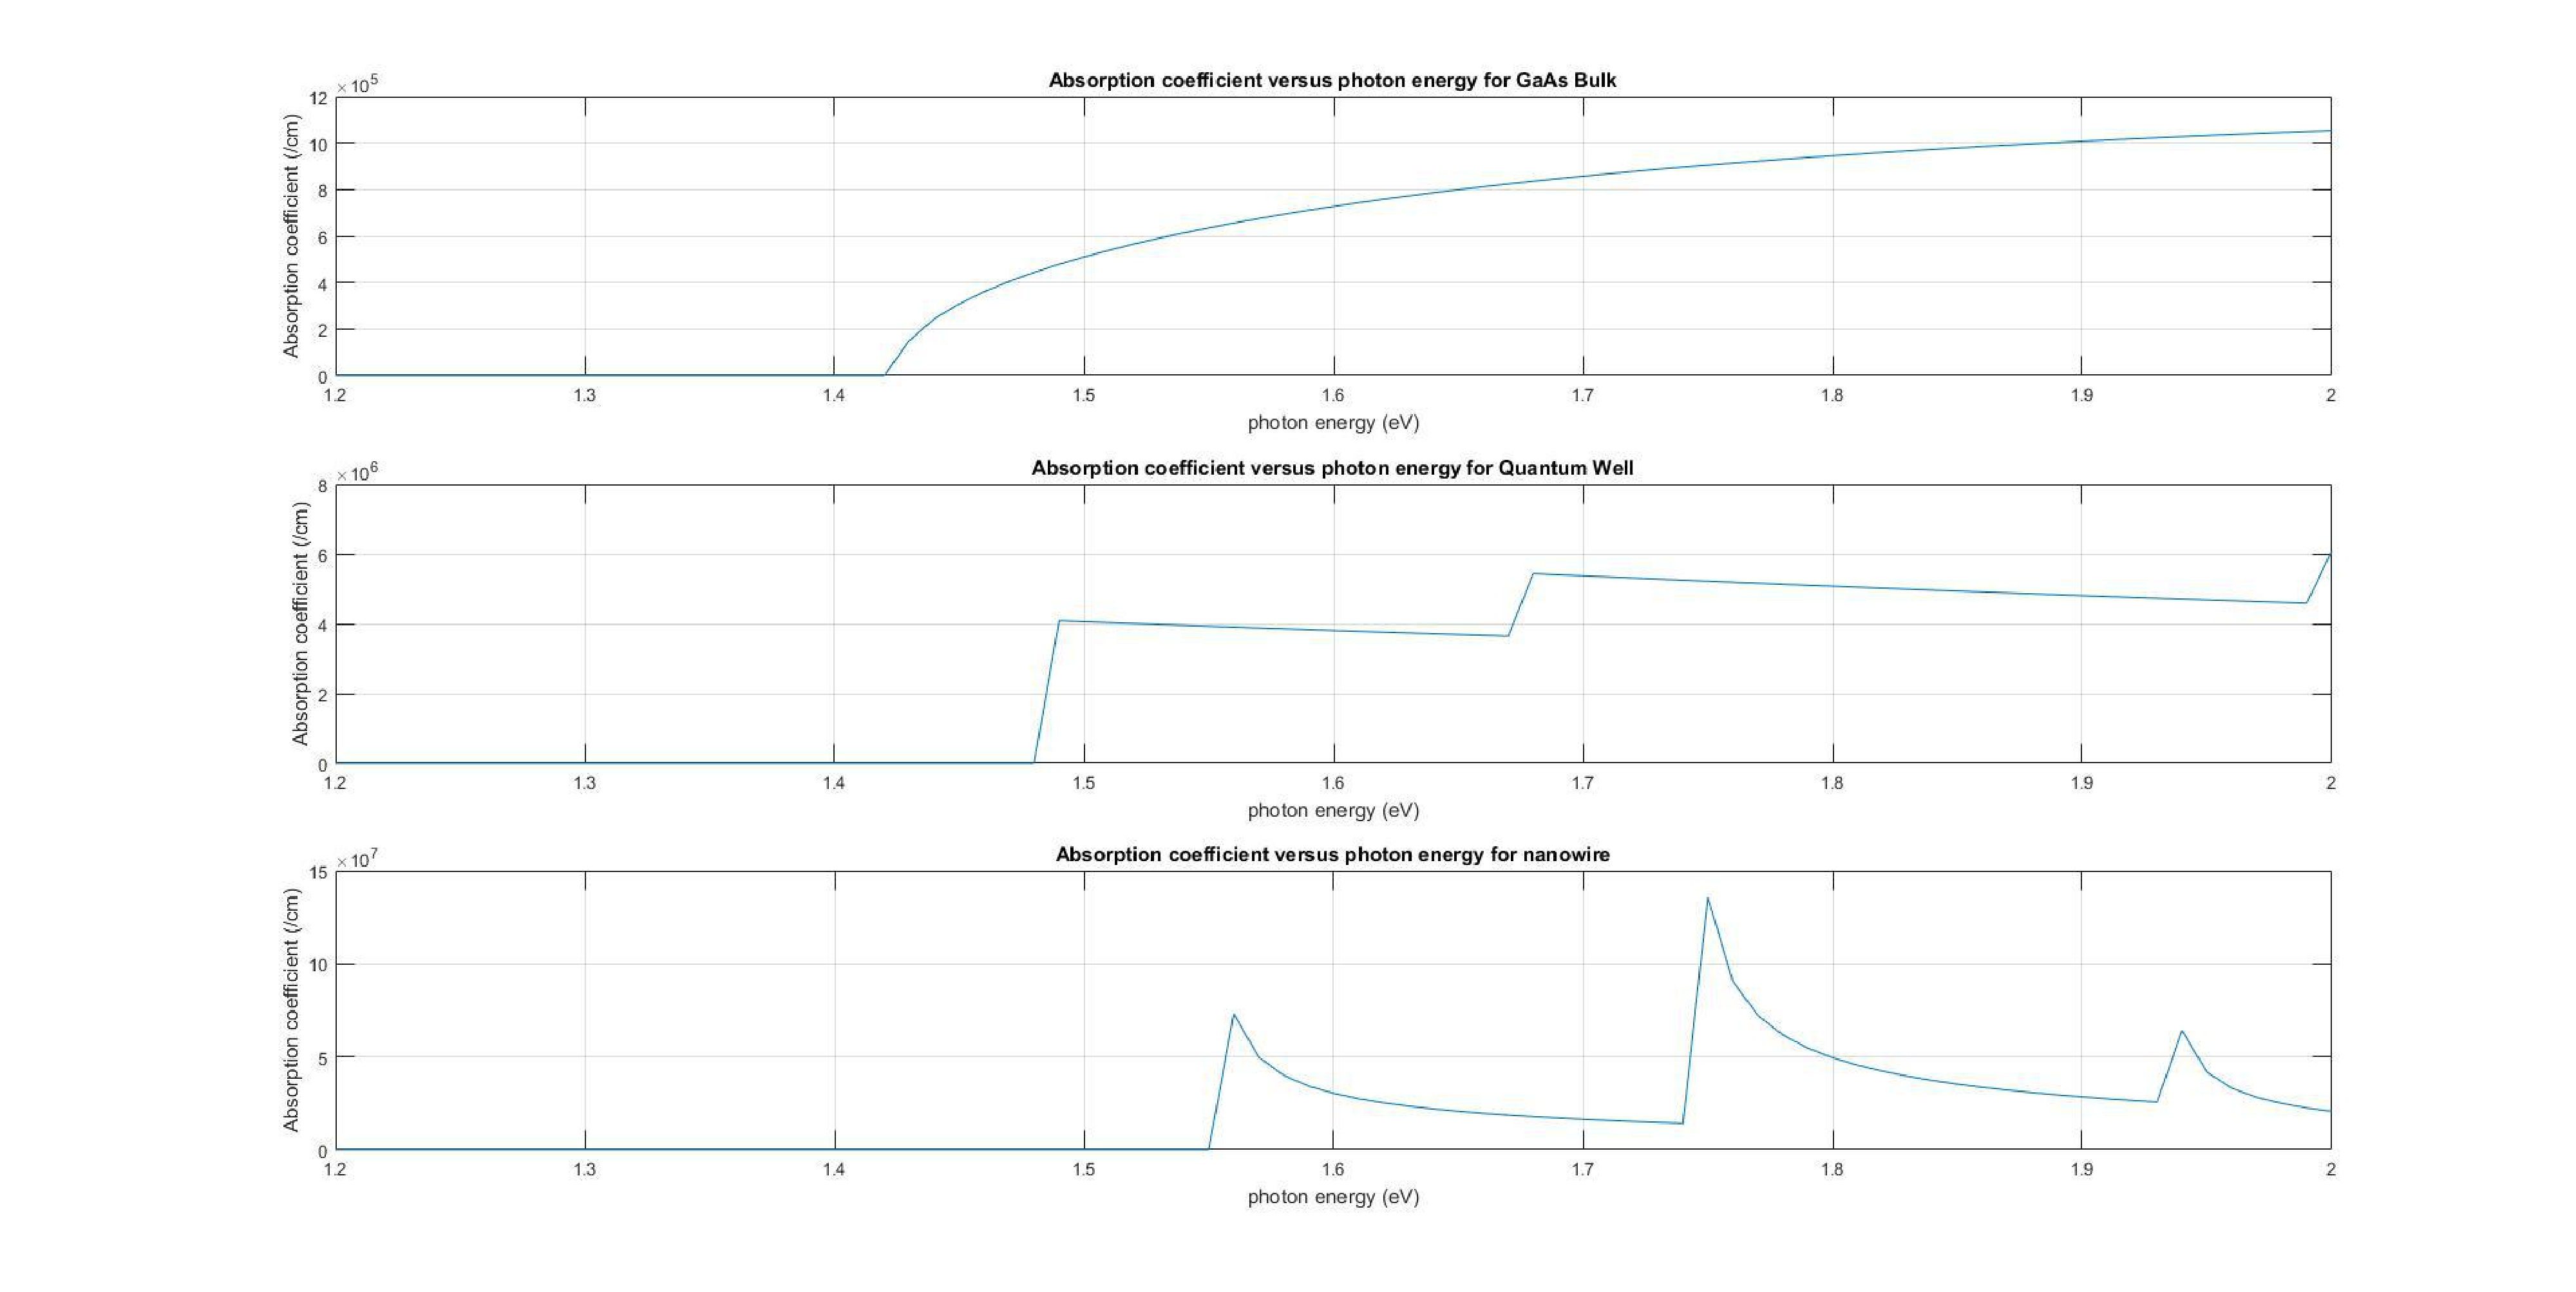
\includegraphics[width=\textwidth]{pictures/LT/absrate_split}
  \label{absrate_split}
\end{figure}

Then the overlay plot with multiple y axis as in Fig.~\ref{absrate_overlay} and
the different scales indicating the enhancement factor for 1D is 35(need to be
verified) compared to 3D.

\begin{figure}
  \caption{Absorption Coefficient versus Photon Energy for 1D 2D and 3D}
  \centering
  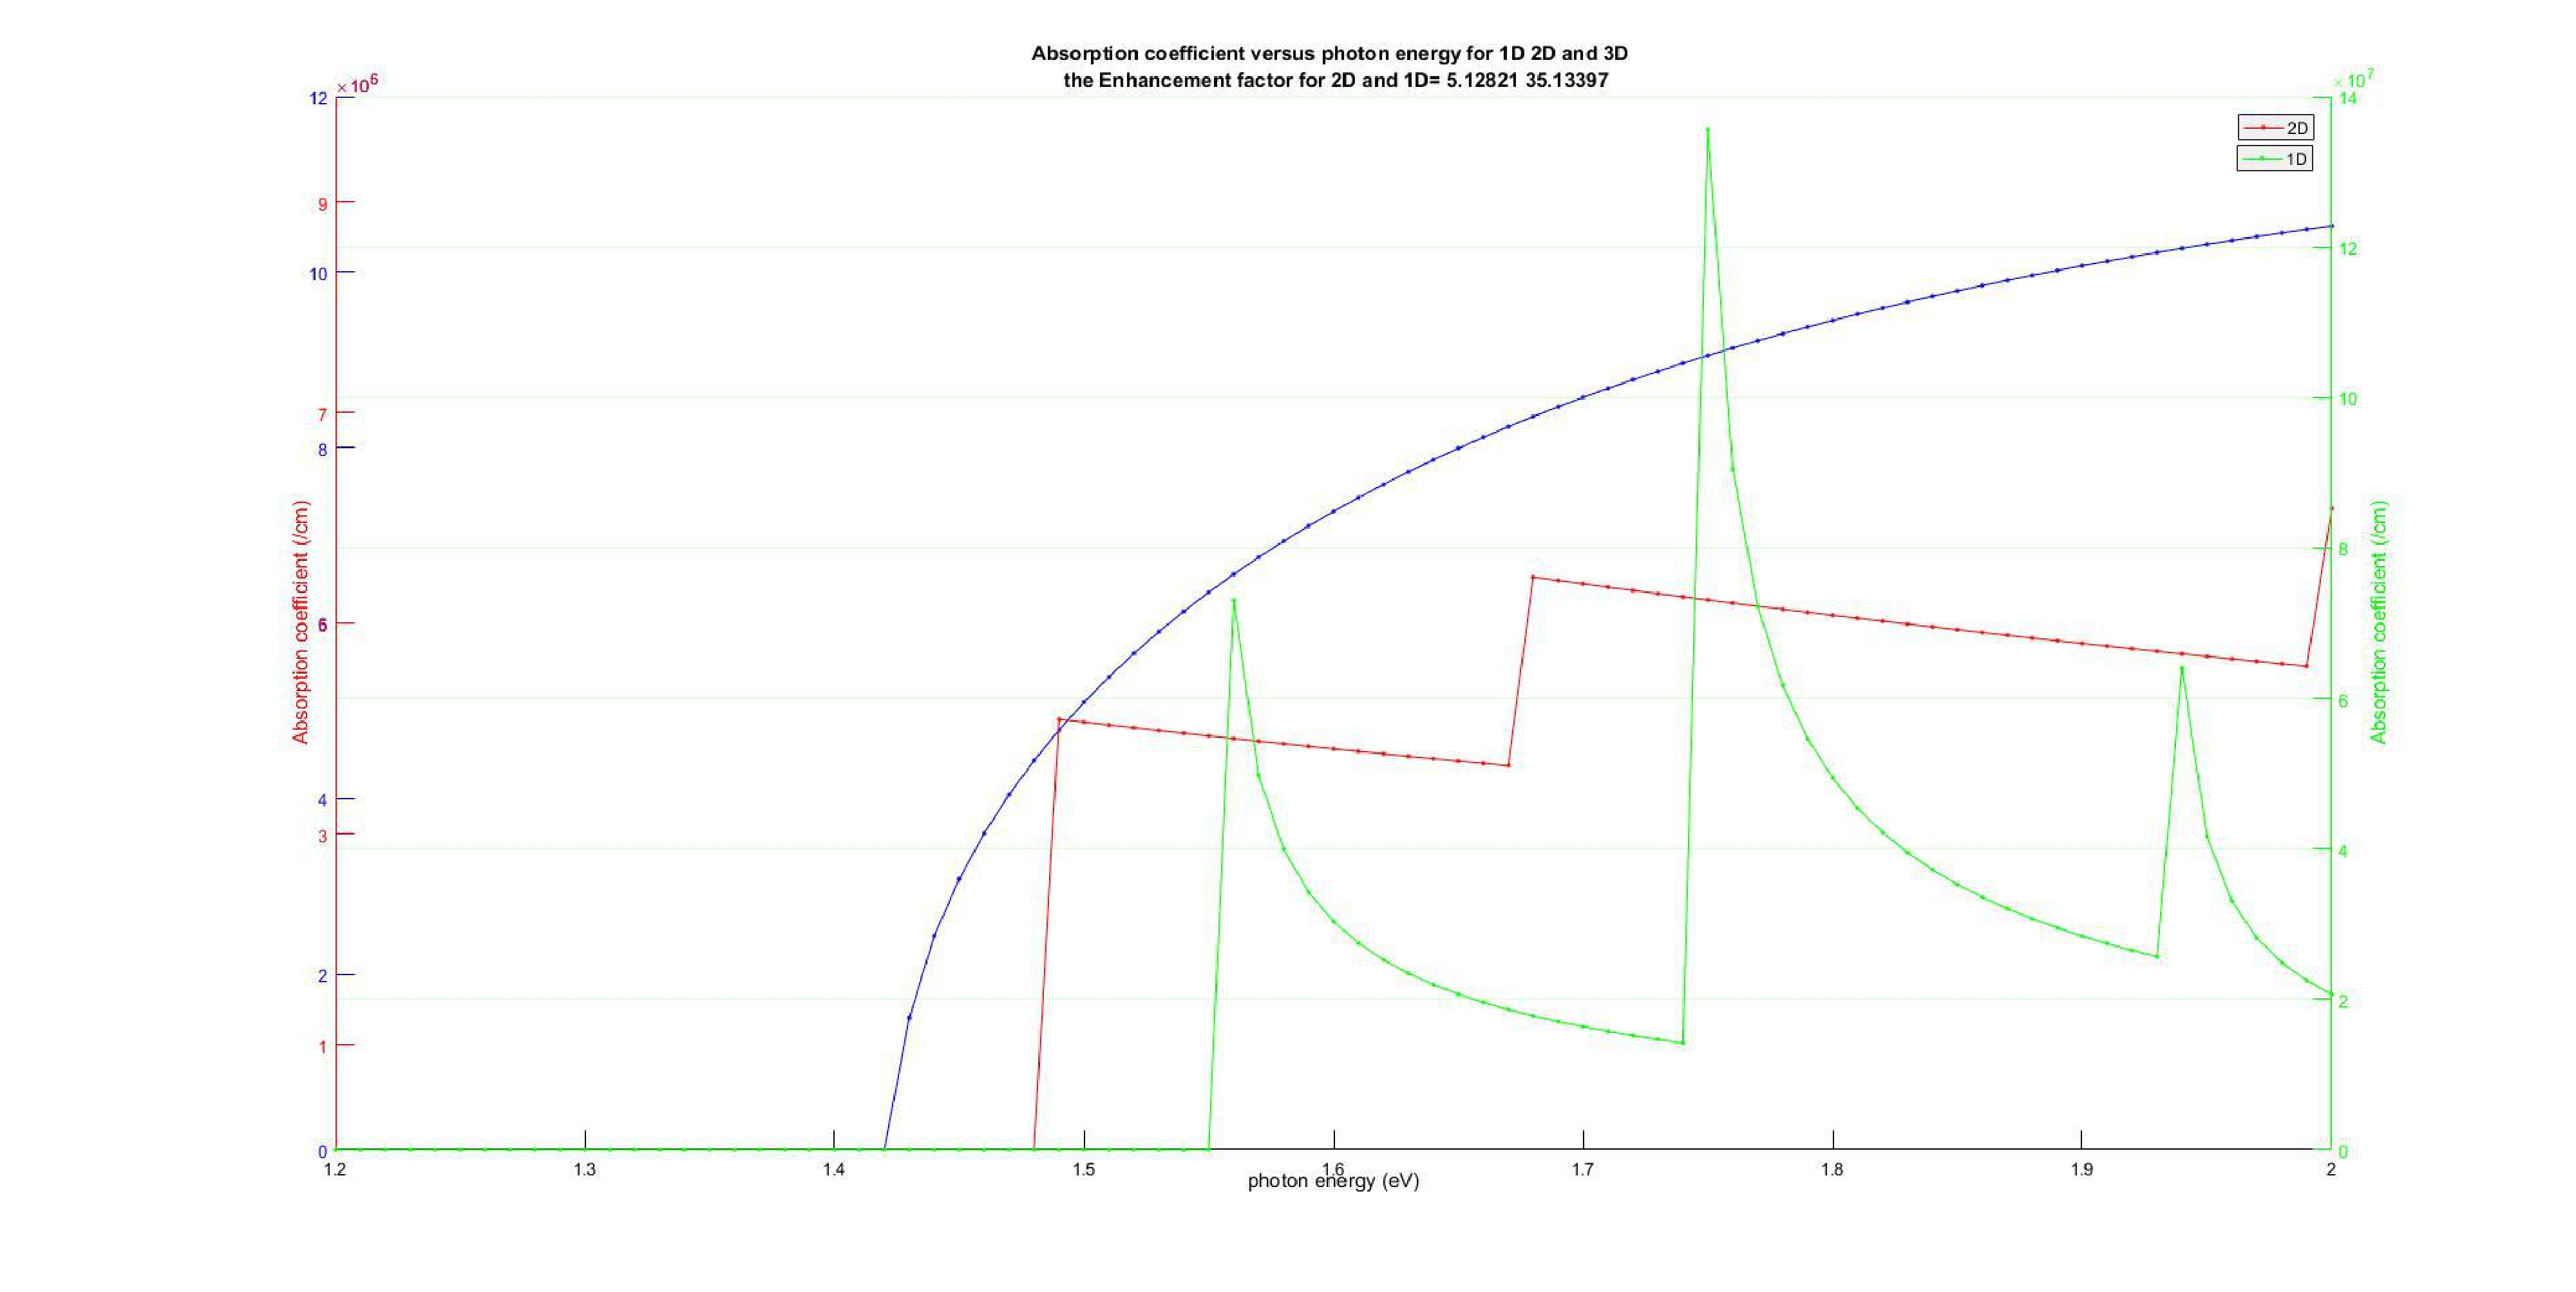
\includegraphics[width=\textwidth]{pictures/LT/absrate_overlay}
  \label{absrate_overlay}
\end{figure}

\subsection{Optical Gain}

Following the treatments of Appendix 3, we can derive the gain spectrum for 3D,
2D and 1D with consideration of occupation factor by calculating the Fermi
levels.

With decreasing dimensionality of the active region of an injection laser, the
density of states and gain spectra become narrower, which leads to a decrease
in the number of states to be filled to make the active region transparent
(zero population inversion and zero gain) and to achieve lasing (gain equal to
loss). Consequently, the transparency current (or inversion current, i.e., the
injection current at which the population inversion is zero) and the threshold
current (injection current at which the gain is equal to the loss and lasing
begins) decrease and their temperature dependences become weaker. The decrease
in the threshold current and increase in its temperature stability reflect one
fo the main areas of development and improvement of injection lasers. Owing to
the continuous nature of the carrier spectrum within the allowed subbands, the
use of QWs or QURs as active medium for optical transitions can only
quantitatively improve the parameters of devices based on them compared with
devices with a bulk active region. 

Among the advantages of QD lasers over the presently used QW lasers are their
narrower gain spectra, much lower threshold currents, and ultrahigh temperature
stability, as well as the wider possibilities for controlling their lasing
wavelength.

All the parameters for rate quations analysis in table~\ref{tab:rate_eq}.

\setlength{\tabcolsep}{4pt}

\begin{deluxetable}{ll}
\tabletypesize{\footnotesize}
\tablewidth{0pt}

\tablecaption{Parameters for rate euqation analysis. \label{tab:rate_eq}}
\tablehead{\colhead{Parameters} & \colhead{Values and Units}}
\startdata
{\em A}   &         $1.43\times10^8~s^{-1}$\\
{\em $\tar_{sp}$}   &   4 ns\\
{\em C}   &         $3.5\times10^{-30}~cm^{6}-s$\\
{\em $n_{g}$}       &   4.2 \\
{\em $\Gamma$}      &   1   \\
\enddata
\tablecomments{This table is available in its entirety in a machine-readable form in the journal publication \citet{Krawczyk:2013}.
A portion is shown here for guidance regarding its form and content.}
\end{deluxetable}


\begin{eqnarray}
\begin{aligned}
  & g_{3D}(\xi)=\frac{\sqrt{2}e^2{m_r^\ast}^{3/2}{p_{cv}^2}}{3{\pi}n_r\epsilon_0{m_0}^2C{\hbar^2}\xi}{\sqrt{(\xi-\xi_g)}}(f_n(\xi_2)-f_p(\xi_1)),
\\
& g_{2D}(\xi)=\frac{e^2{m_r^\ast}{p_{cv}^2}}{3{n_r}\epsilon_0{m_0}^2C{\hbar}L_z\xi}(f_n(\xi_2)-f_p(\xi_1)),
\\
& g_{1D}(\xi)=\frac{e^2{m_r^\ast}^{3/2}{p_{cv}^2}}{3{n_r}\epsilon_0{m_0}^2C\xi{L_x}{L_y}}\frac{1}{\sqrt{(\xi-\xi_g)}}(f_n(\xi_2)-f_p(\xi_1)),
\end{aligned}
\label{eq:five}
\end{eqnarray}

Now we can plot the gain spectrum respect to photon energy for 3D, 2D and 1D in
the figure below. As we can see, the gain spectrums follow the unique shapes of
density of states. The fourth figure is the maximum gain versus electron
carrier concentration varing from $3\times10^{18} (cm^{-3})$ to
$3\times10^{19}(cm^{-3})$. Using parameters $N_{tr} = 2\times10^{18} cm^{-3}$,
$N_{s} = 4\times10^{18} cm^{-3}$, and $g_0 = 6.11\times10^{5} cm^{-1}$, we fit
the curve in Fig.~\ref{gainspectrum} to build a logarithmic gain model of the
form for 3D case:

\begin{equation}
  g(N) = g_0\ln\left(\frac{N+N_s}{N_{tr}+ N_s}\right)
\end{equation}

where $N_s$ is a shift to force the natural logrithm to be finite at $N = 0$
such that the gain equals the umpumped absorption due to the band-to-band
transitions, $N_{tr}$ is the transparency carrier density, and $g_0$ is the
gain coefficient. $N_{tr}$ and $g_0$ will be different for different
dimensionality.

\begin{figure}
  \caption{Gain Coefficient versus Photon Energy for 1D 2D and 3D}
  \centering
  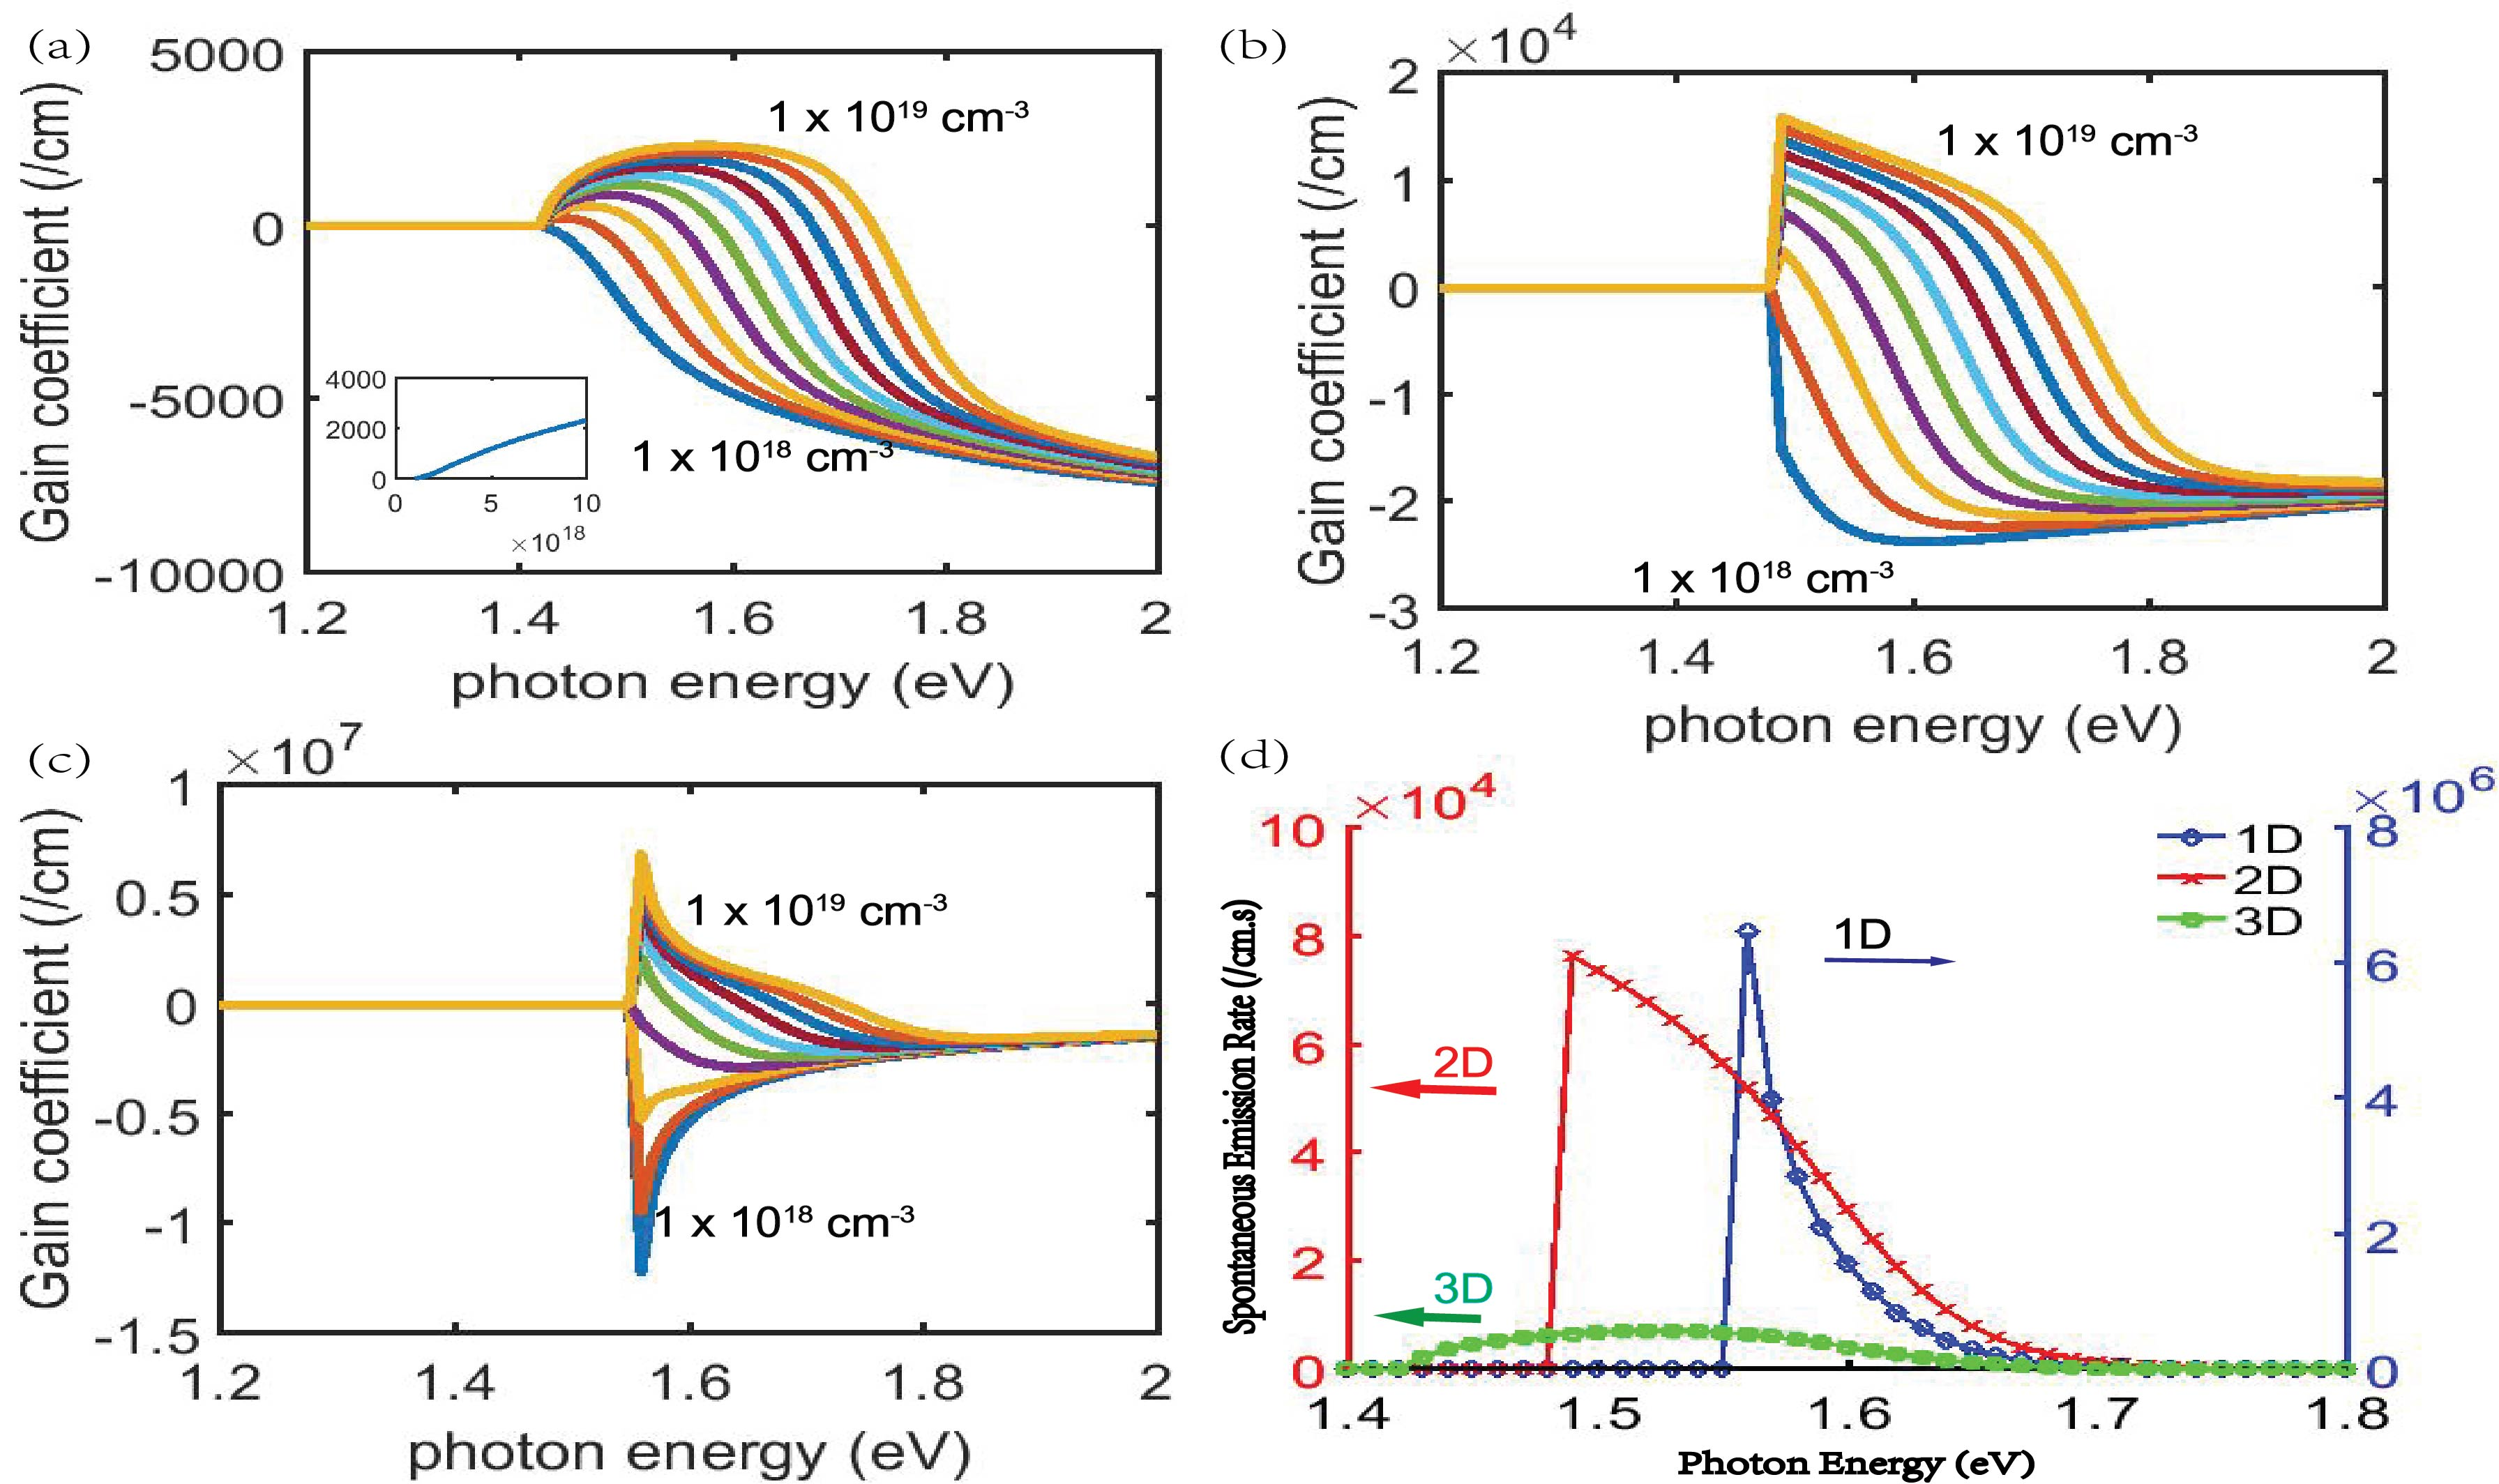
\includegraphics[width=\textwidth]{pictures/LT/gainspectrum}
  \label{gainspectrum}
\end{figure}

\begin{figure}
  \caption{Gain Model Fitting}
  \centering
  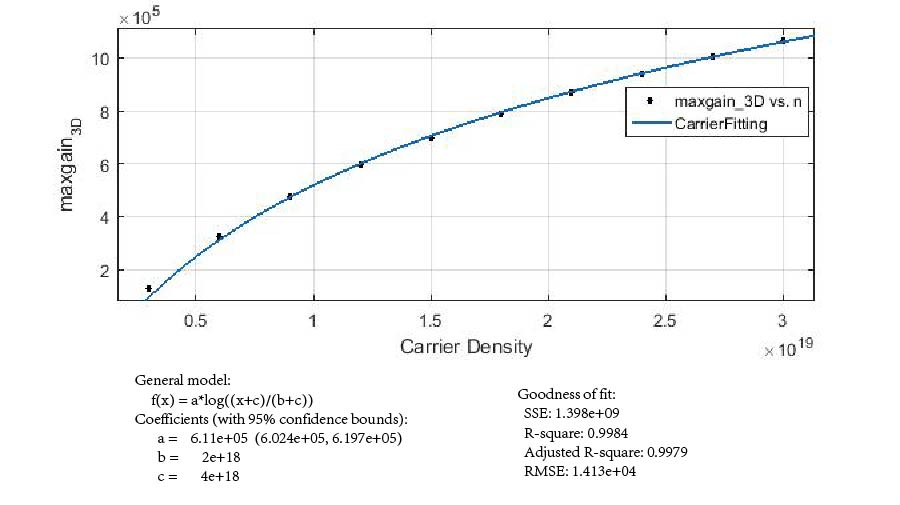
\includegraphics[width=\textwidth]{pictures/LT/gainModelFit_Anoted}
  \label{gainModelFit_Anoted}
\end{figure}

After fitting the curve in Fig.~\ref{gainModelFit_Anoted}, we can calculate the
threshold carrier density is $N_{th} = 4.533\times10^{18} cm^{-3}$. Then
plotting the spontaneous emission rate with respect to the threshold carrier
density $N_{th}$ for 3D, 2D and 1D as following: 

\begin{eqnarray}
\begin{aligned}
& r_{3D}^{\mathrm{spon}}(\xi)=\frac{n_re^2\xi{p_{cv}^2}}{{\pi}\epsilon_0{m_0}^2C^3{\hbar^2}}\frac{{m_r^\ast}^{3/2}}{2\pi^2\hbar^3}{\sqrt{(\xi-\xi_g)}}f_n(\xi_2)(1-f_p(\xi_1)),
\\
& r_{2D}^{\mathrm{spon}}(\xi)=\frac{n_re^2\xi{p_{cv}^2}}{{\pi}\epsilon_0{m_0}^2C^3{\hbar^2}}\frac{{m_r^\ast}}{\pi\hbar^2L_z}f_n(\xi_2)(1-f_p(\xi_1)),
\\
& r_{1D}^{\mathrm{spon}}(\xi)=\frac{n_re^2\xi{p_{cv}^2}}{{\pi}\epsilon_0{m_0}^2C^3{\hbar^2}}\frac{{m_r^\ast}^{3/2}}{\pi\hbar{m_e^\ast}L_xL_y}\frac{1}{\sqrt{(\xi-\xi_g)}}f_n(\xi_2)(1-f_p(\xi_1)),
\end{aligned}
\label{eq:six}
\end{eqnarray}

\begin{figure}
  \caption{Spontaneous Emission Rate versus Photon Energy for 1D 2D and 3D}
  \centering
  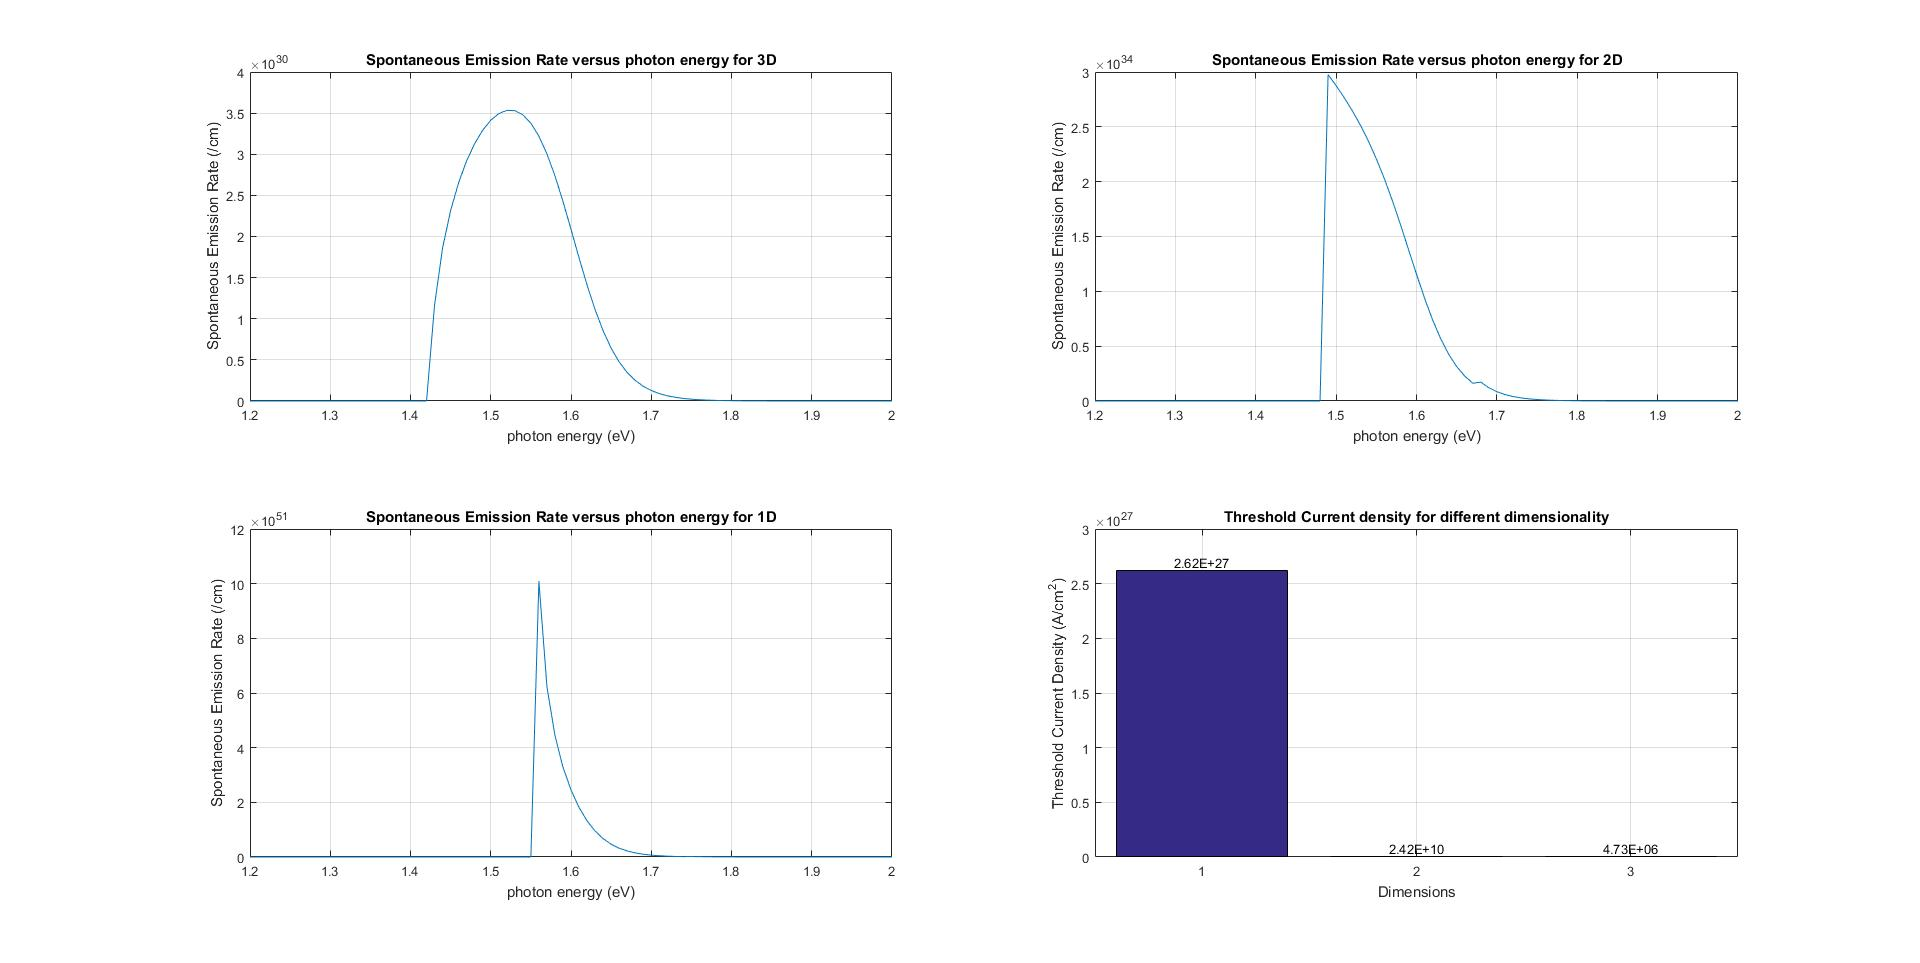
\includegraphics[width=\textwidth]{pictures/LT/sponrate}
  \label{sponrate}
\end{figure}

Integraing over all the photn energy spectrum, we have $R_{sp} =
\int_{\xi}r_{sp}d{\xi}$ for different dimensionality, then the threshold
current density can be simply caluclated as: $J_{th}= qdR_{sp}|_{N_{th}}$ and
plotted in the fourth part of Fig.~\ref{sponrate}. The threshold current for 3D
is $2.62\times10^{27} (A/cm^2)$, 2D is $2.42\times10^{10} (A/cm^2)$, and 1D
case is $4.73\times10^{6} (A/cm^2)$. The threshold current density needed for
lower-dimensional structure is greatly reduced.

Next, we can do dynamic analysis of laser modal and replace the threshold
current density to threshold pumping power. And verify the result with the
experimental data.

\subsection{Feedback and Laser Threshold}
\section{Types of semiconductor Lasers} \label{corrections}
\subsection{Fabry-Perot Semiconductor Lasers}

The Fabry-Perot(FP) laser is conceptually just an LED with a pair of end
mirrors or facets. The mirrors are needed to create the right conditions for
lasing to occur. The lasing medium can only amplify (undergo stimulated
emission) over a fairly narrow range because of the characteristics of the
material it is made from . A typical gain curve is illustrated on the
left-hand. 

\subsection{Grating-Based semiconductor Lasers}
\subsection{Vertical-Cavity Surface-Emitting Lasers}

As seen, light in the VCSEL propagates vertically with DBR mirrors as the
nature of the manufacturing process, the entire round-trip of the VCSEL is much
shorter than that of with the edge-emitting lasers. It leads to high
reflectivity ( around 99.9$\%$) of DBR mirrors, in which the large number of
layers are required.

One of features related to the VCSELs is the longitudianl modal stability due
to its short cavity length (around order of the wavelength). A

\subsection{Grating Surface-Emitting Lasers}
\section{Characteristics of Semiconductor Lasers} \label{corrections}

In order to understand their operation, it is necessary to know some basic
performance parameters or important features of semiconductor lasers.

\section{Basic Requrement for Design of Semiconductor Lasers} \label{corrections}
\subsection{Spectral width and Linewidth}

FP semiconductor lasers produce a range of wavelengths. This range of
wavelengths is called the "spectral width" of the laser. Typically there will
be around 8 "modes" and the spectral width. In order to determin exactly the
spectral shape, spectral width is usually quoted as the FWHM (Full Width Half
Maximun) Instead of producing a continuous range of wavelengths over their
spectral width. Semiconductor lasers produce a series of "lines" at a number of
discrete wavelengths. Lines themselves vary in width (in different types of
lasers) very significantly. The linewidth is inversely proportional to the
coherence length of the laser.

\subsection{Operating Wavelength, Switching Time, and Modulation}
\section{Modeling of Semiconductor Lasers} \label{corrections}

From the general formulations through the rate equations ans wave equations
based on the

As we know, from different aspects of the same physics of the energy
conservation, there are two basic classical methods to model the operation of
semiconductor lasers. The first method, which will be summarized , applies the
concept of photo/electron particle exchange with the abtract optical parameters
and is suitable for the FP lasers. For the DBR/DFB lasers, due to strong
non-uniformities of index distribution. The interaction between electromagnetic
fields and electric particles has been considered, which . Indeed, those two
methods are wholly compatible with one anohter. In this project, because we
focus on the FP lasers as , we employ the first method: the standard rate
equation approach.

Three fundamental elements in the semiconductor lasers: semiconductor band
structure, current injection, and cavity. The former two are related to the
material and junction structure, and the later is related to the laser
structure. For semiconductor lasers, the key in the modeling is to deal with
the interaction between electromagnetic fields and gain medium. The basic
procedure of modeling of semiconductor lasers: Due to the complexity of the
rate equation and coupling between carrier and photon density, the coupling
rate equations are further solved by numerical methods such as the
standing-wave approach (in frequency domain) and the traveling-wave approach
(in time domain). The stading-wave approach is based on the assumption that the
temporal and the spatial dependence of field distributions of the cavity odes
are separable. As such, the dynamics is considered in the modal amplitudes.
Consequently, the standing-wave apporach is valid only when the photon lifetime
is much shorter than the characteristic time of the laser dynamics. The
traveling-wave approach, on the other hand, makes no assumptions about the
cavity modes. Rather, it solves the time-dependent coupled=wave equations for
the forward and the backward traveling waves directly and tehrefore is valid
even the laser cavity has relatively small Q-factor and/or the characteristic
time of the laser dynamics is very short. Another advantage of the
traveling-wave model is that it can be readily applied to laser diodes operated
with multiple cavity modes, for which the stading-wave model may have
difficulty in finding the complex roots corresponding to each mode.
\section{Laser Rate Equations} \label{corrections} 


We start with the governing equations of carrier density and photon density in
the active region which is governed by a dynamic process.

\begin{eqnarray}
\begin{aligned}
  & \frac{dN}{dt} = \frac{\eta_{i}I}{qV} - \frac{N}{\tau} - R_{st},
  \\
  & \frac{dN_p}{dt} = {\Gamma}v_g{g}N_p + \Gamma\beta_{sp}R_{sp} - \frac{N_p}{\tau_p},
\end{aligned}
\label{eq:eight}
\end{eqnarray}

where $\beta_{sp}$ is the spontaneous emission factor, defined as the
percentage of the total spontaneous emission coupled into the lasing mode. And it is
just the reciprocal of the number of available optical modes in the bandwidth of
the spontaneous emission for uniform coupling to all modes. The g is Incremental gain
per unit length.

The first term of equation 1 is the rate of injected electrons $G_{gen} =
{\Gamma_{i}I}/{qV}$, ${\Gamma_{i}I}/{q}$ is the number of electrons per
second being injected into the active region, where V is the volume of the
active region. The rest terms are the rate of recombining of electrons per unit
volume in the active region. There are several mechanisms should be considered,
including a spontaneous recombination rate, $R_{sp}$, a nonradiative
recombination rate, $R_{nr}$, a carrier leakage rate, $R_l$ and a net
stimulated recombination, $R_{st}$, including both stimulated absorption and
emission. Which looks like:

\begin{equation}
  R_{rec} = R_{sp} + R_{nr} + R_{l} + R_{st}
\end{equation}

The above equation used input current intensity, $I$, for electrically injected
lasing situation, however, if optical pump used as the lasing source, then we
need to rewrite the governing equations.

\begin{eqnarray}
\begin{aligned}
  & \frac{dN}{dt} = \frac{\eta_{i}P}{qV} - \frac{N}{\tau} - R_{st},
  \\
  & \frac{dN_p}{dt} = {\Gamma}v_g{g}N_p + \Gamma\beta_{sp}R_{sp} - \frac{N_p}{\tau_p},
\end{aligned}
\label{eq:eight}
\end{eqnarray}

$P$ is the optical pump used for exciting nano-cavity laser emission and is
time-dependent of the form $P_{p}sech^2(\frac{1.76t}{\delta{t}})$, where $P_p$ is the peak power amplitude, and $\delta{t}$ is the time pulse width.


The cavity loss can be characterized by a photon decay constant or lifetime,
$\tau_p$, and the gain necessary to overcome losses, and thus reach threshold.
By assuming steady-state conditions (\ie $dN_p/dt = 0$), and solving for this
steady-state or threshold gain, $g_{th}$, where the generation term equals the
recombination term for photons. We assume only a small fraction of the
spontaneous emission is coupled into the mode (\ie $\beta_{sp}$ is quite
small), then the second term can be neglected, and we have the solution:

\begin{equation}
  \Gamma{g_{th}} = \frac{1}{v_g\tau_p} = <\alpha_i> + \alpha_m
\end{equation}

The product, $\Gamma{g_{th}}$, is referred to as the threshold modal gain
because it now represents the net gain required for the mode as a whole, and it
is the mode as a whole that experiences the cavity loss. $<\alpha_i>$ is the
average internal loss, and $\alpha_m$ is the mirror loss if we considered an
in-plane wave laser.

\begin{equation}
  R_{rec} = R_{sp} + R_{nr} + R_{l} + R_{st}
\end{equation}

The first three terms on the right refer to the natural or unstimulated carrier
decay processes. The fourth one, $R_{st}$, require the presence of photon.


Then, recognizing that $(R_{sp} + R_{nr} + R_{l}) =AN + BN^2 +CN^3$ depends
monotonically on $N$, we observe from eq 2.34 that above threshold $(R_{sp} +
R_{nr} + R_{l})$ will also clamp at its threshold value, given by Eq 2.35. Thus,
we can substitute Eq 2.35 into the carrier rate equation, eq 2.16 to obtain a
new above threshold carrier rate equations,

\begin{equation}
  \frac{dN}{dt} = \eta_i \frac{(I - I_{th})}{qV} - v_{g}gN_p,~~~   (I > I_{th})
\end{equation}

We also calculate a steady-state photon density above threshold where $g = g_{th}$,

\begin{equation}
  N_p = \frac{\eta_i (I - I_{th})}{qv_{g}g{th}V}~~~   (steady~ state)
\end{equation}

To obtain the power out, we first construct the stored optical energy in the
cavity, $E_{os}$, by multiplying the photon density, $N_p$, by the energy per
photon, $hv$, and the cavity volume, $V_p$. That is $E_{os} = N_phvV_p$. Then,
we multiply this by the erngy loss rate through the mirrors, $v_g\alpha_m =
\frac{1}{\tau_m}$, to get the optical power output from the mirrors,

\begin{equation}
  P_0 = v_g\alpha_{m}N_phvV_p
\end{equation}

Substituting from , and using $\Gamma = V/V_p$,

\begin{equation}
  P_0 = \eta_i(\frac{\alpha_m}{<\alpha_i> + \alpha_m})\frac{hv}{q}(I - I{th}),~~~(I > I_{th})
\end{equation}


We can get the threshold carrier density

\begin{equation}
  N_{th} = N_{tr}e^{g_{th}/g_{0}N} = N_{tr}e^{(<\alpha_i> + \alpha_m)/\Gamma{g_{0}}N}
\end{equation}

Using the polynomial fit for the recombination rates, and recognizing that for
the best laser material the recombination at threshold is dominated by
spontaneous recombination, we have, $I_{th}\cong B{N_{th}}^2qV/\eta_i$, Thus

\begin{equation}
  I_{th} {\cong} \frac{qVB{N_{tr}}^2}{\eta_i}e^{(<\alpha_i> + \alpha_m)/\Gamma{g_0}N}
\end{equation}

where for most $\uppercase\expandafter{\romannumeral3} -
\uppercase\expandafter{\romannumeral5}$ materials the bimolecular recombination
coefficient, $B \sim 10^{-10} cm^3/s$.

Reduce the transparency value and increase the differential gain of the active
materials.

It is desirable to reduce the cavity loss $(<\alpha_i> + \alpha_m)$ and volume,
$V$, in order to retaining a reasonably large confinement factor, $\Gamma$.

\section{Wave Model of Semiconductor Lasers} \label{corrections}

\section{Linewidth Enhancement Factor} \label{corrections}

Electrons and holes frequently interact with other carriers and with phonons,
thereby changing their energy within the sub-band. Such intra-band scatter
events happen about every 0.1 ps, much more often than band-to-band
recombination events. Thus, scattering leads to an uncertainty of the electron
energy, which can be accounted for by introducing a symmetrical linewidth
broadening funtion L into the gain formula.  This convolution integral means
that gain at the photon energy can now receive contributions from electron
transitions with, weighted by 

In fact, positive gain is now possible even for photon energies slightly below
the bandgap. Cauchy himself exploited such a density function in 1827, with
infinitesimal scale parameter, in defining a Dirac delta function, while among
physicists, it is known as the Lorentzian line shape functionL with the
half-width. This function is based on the assumption that the occupation
probability of an electron state decays proportionally to exp(-t/). The Fourier
transformation of this exponential function into the nergy domain leads to .
Gamma is the average of the broadening in the conduction and inthe valence
band. The full linewidth 2gamma is related to the average intra-band scattering
time 

Which includes scattering events in the conduction band and valence band. For
each band, linewidth contributions from different scattering processes are
adding up.

\section{Implementations} \label{corrections}
\subsection{Optical Modes}
\subsection{Steady State Analysis}
\subsection{Dynamic State Analysis}

\section{Simulation Results} \label{corrections}
\subsection{Input Parameters}
\subsection{Optical Modes}
\subsection{Steady State Analysis}
\subsection{Dynamic State Analysis}

  
  %CHAPTER: Conclusion
  \chapter{Conclusions and Future Research} \label{conclusions}

As mentioned previously, communication of information, together with storage
and computation form a “grand challenge” of the information age [2, 7].
Recently, the analysis of big data has become the engine for societal,
financial, scientific, and technological endeavors. This demands an
infrastructure that is capable of fast and reliable high volume data
processing. Traditionally, this requirement was fulfilled by silicon
technology. However, silicon-based technology has its own limitations, such as
speed limit and heat dissipation problem. In order to process high volume data,
we need data computation, storage and communication work as three fundamental
functions of a computation cell. A monolithic nano-system may be envisioned
which incorporates NWs as waveguides, detectors, photovoltaic cells, antennas,
modulators, (photo)capacitors, LEDs, and lasers, .These components may be
incorporated in circuit layers, such as network on chip. Different layers can
communicate using NW through-silicon vias (TSVs). Similar
low-power/high-performance advantages can be realized through achievement of
high interconnect densities on the 2.5D Though-Si-Interposer (TSI) as reported
in [114].

In conclusion, optical properties of nano-cavities were reviewed
here emphasizing the analysis of resonant optical modes which depend both
radially and axially on the geometries of the nanowires. This shows how such
sub-wavelength structures can form optical cavities as-grown, without needing
sophisticated facet mirrors. In addition, we show how the fortuitous overlap of
the reduced dimensional electronic wave functions and the photonic modes is
responsible for the extraordinary optoelectronic properties of core-shell
nanowires. Such nano-structures have been developed on heterogeneous
substrates, particularly silicon, and as such becoming an important component
in the next generation of photonic integrated circuits which are particularly
useful in meeting the grand challenge of low energy and fast speed computation.

\section{Contributions of this dissertation}

In this dissertation, we simulated the two-dimensional-electron-gas based
heterostructure . and compared it with undoped structure. The static behavior
simulations, including 2-D potential profile, electric field distributions, and
carrier concentration, were performed with commercially availabe software. The
carrier transient behaviro in the absorption region was investigated by . The
simulation revealed the vertical field in the absortpion region enhanced the
elctron transport. 

We showed that two-dimenisonal gas can work as an extended contact to collect
photogenerated carriers by means of carrier-carrier scattering which results in
a fast energy relaxation time.

In addition, we designed a 2DEG/@DHg structure based high-speed photodetector
on GaAs substrate for optical communication applictions. It takes the
advantages of both vertical field and confined 2D gas, and transforms a lateral
MSM structure. 

The major contributions of this thesis are (1) simulation and analysis the 2DEG
device, revealing a vertical field in the absorption region which facilitates
electron transportl; (2) design, simulation and analysis of 2DEG based MSM
phototedtector.

\section{Outline of the future work}

%Insert amazing opening paragraph here.  An overview of the goals of this thesis.
%General idea: Take a group of observables, look for correlations, relate to physics.

Low dimensional electron gases exsit at the heterointerfaces of core-shell
nanowires (CSNWs). For example, the GaAs/AlGaAs CSNWs typically form a
hexagonal structure in which six (6) pillars of 1D charge at the vortices, and
six (6) sheets of 2D charge at facets  are formed~\cite{Wang:2015hz}. At the same time,
nanowires (NW) have also been shown to be capable of confining light in their
sub-wavelength nano-structure, supporting photonic modes, and producing
resonant cavities without the need for polished end facets. We have previously
shown how the electronic wave functions that are thus formed affect the optical
transition rates, resulting in orders of magnitude  enhancement in absorption
and emission of light. Here we report on the plasmonic effects of the
confined charge on the optical properties of CSNWs We report on finite
difference time domain (FDTD) simulations with the aim of identifying the
surface plasmon resonance modes which affect light confinement in hexagonal
CSNWs, and help form a  high quality factor resonant cavity. This is done by
comparing regular CSNW, with a) wires covered with metal which produces surface
plasmon-polaritons (SPP’); b) NWs covered with metal that is sandwiched between
the core and the outer, shell; and c) two-dimensional electron gas (2DEG)
which  embedded at the heterointerace of CSNWs. Results show that the 2DEG
behaves similarly to an embedded metallic surface, allowing for highly
localized light confinement in these wires without the need for vertical
structures such as Bragg mirrors commonly used in vertical cavity surface
emitting lasers (VCSEL’s). Besides affecting the cavity, the 2DEG enhances  the
transition rates due to the plasmon-electron interaction, facilitating not only
photonic stimulated emission and lasing, but also  surface plasmon
amplification by stimulated emission of radiation~\cite{Bergman:2003vo}.

We model the dielectric function of the two dimensional electron gas using the
Drude model for dispersive media, and extract its relevant parameters from~\cite{Bergman:2003vo}.
The complex conductivity of the 2DEG is derived using the relaxation time
approximation, effective reduced mass of electrons, and the density of the
carriers in the gas. By substitution the complex conductivity in Drude model,
we can model the 2DEG, with given plasma frequency, damping coefficient, and
the oscillator strength using FDTD simulator.

The two dimensional plasma frequency is calculated as~\cite{Bergman:2003vo}: in which,  is the
background dielectric constant and m* is the effective mass of the electron. It
is important to note that, as shown in (1), the plasma frequency of the 2DEG
can be tuned with changing the carrier concentration. This tubnability
distinguishes the 2DEG from other plasmonic material such as metals. The
complex conductivity of the electron gas is derived as~\cite{Bergman:2003vo}:

The electromagnetic wave traveling of the Surface Plamon Polariton (SPP)
involves both charge motion in electron reservoir (e.g., metal, graphene and
2DEG) and waves in the dielectric or air. Instead of using any metallic
materials, Core-Shell nanowires (CSNWs) can naturally form two-dimensional
electron gas (2DEG) at the heterojunction interface and even large
one-dimensional pillar of charge at the corners of thier hexagonal facets.

Surface plasmon polaritons are density oscillations of electrons at the surface
of a dielectric. Noble metals such as Au and Ag are considereed as the best
plasmonic material candidates because of their high conductivity and low loss.
The important parameters fro choosing the metals in plasmonic nanowire are the
relaxation time and the plasma frequency of the metallic layer. Since silver
has the smallest relaxation time, we coat a CSNW with it in order to study its
effect on the NW cavity. we futhre embed Ag between the GaAs core and AlGaAs
shell and compare its affect on the field profile and mode generation. Finally,
we compare this configuration with a relatively dense 2DEG which is formed at
the heterointerface of CSNWs. Simulation is performed using MIT's MEEP open
source finite-differnce time-domain (FDTD) simulation software.  For modeling
the 2DEG we use data in , and for metallic layers, we used Lorentz-Drude model
based on experimental data extracted from.

\begin{figure}
  \caption{An FDTD-simulated electric field profile (linear scale) of (a) a hexagonal core-shell nanowire (CSNW), (b) photonic modes are affected by plamonic modes in a CSNW covered with silver coating, (c) CSNW with embedded silver layer between the core and the shell; (d) plasmonic and photonic modes of CSNW with embedded 2DEG show similar effects compared to embedded metal. The black boundaries represent the interface betweeen layers of the structure.}
  \centering
  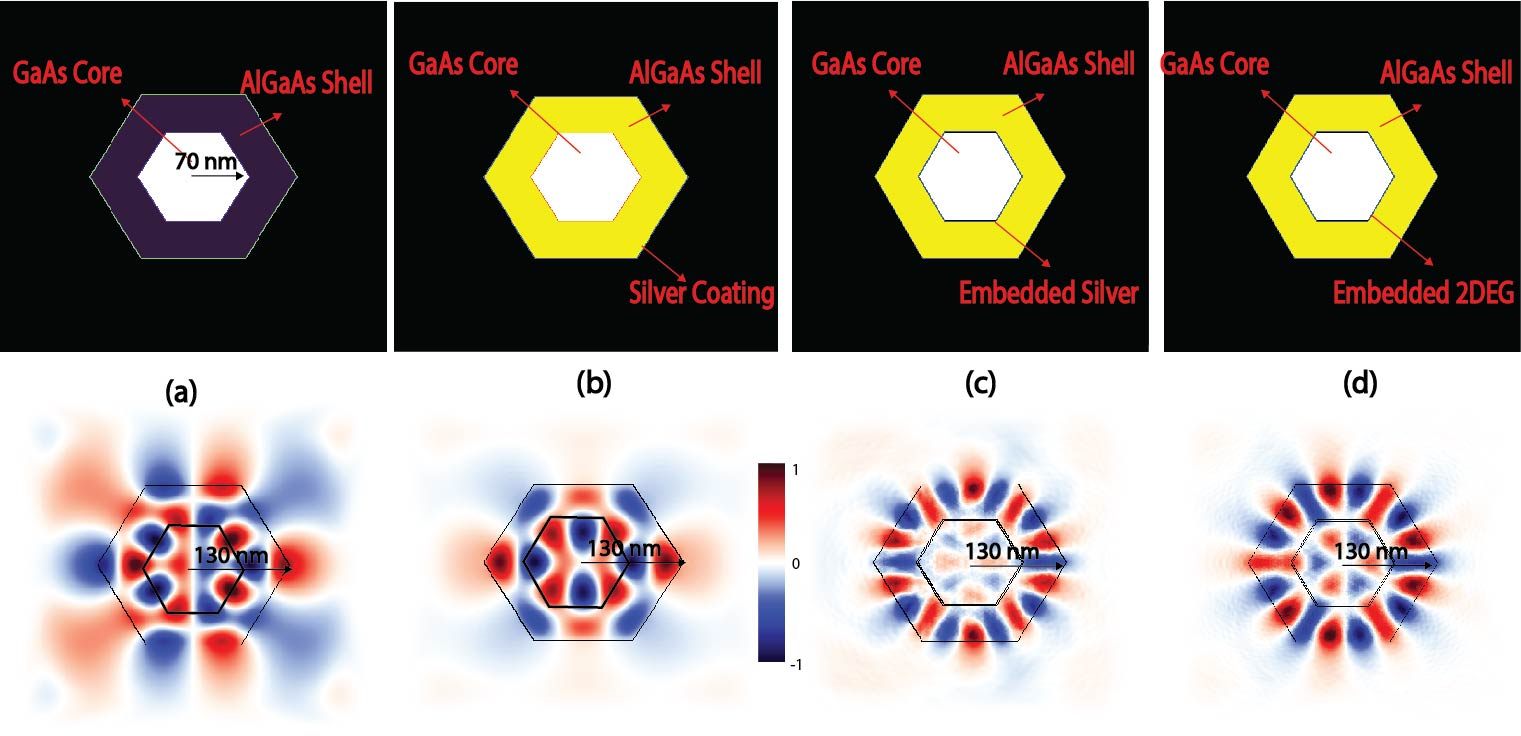
\includegraphics[width=\textwidth]{pictures/Conclusion/PlasmonMode}
  \label{PlasmonMode}
\end{figure}

Figure~\ref{PlasmonMode} shows the FDTD-simulated electric field profile (linear scale) in the
transverse plane of (a) CSNW; (b) CSNW with silver coating; (c) CSNW with and
embedded silver layer between the core and the shell; (d) CSNW with 2DEG at the
hetero-interface. As shown in Fig, coating the wire with metal introduces
plasmonic modes in the structure that enhance light confinement. Metal embedded
betweeen the core and the shell has similar effect. Importantly, we observe
that similar plasmonic features can be obtained due to the 2DEG that is
embedded in CSNW~\cite{montazeri2016plasmonic}.

Recently, the analysis of big data has become the engine for societal,
financial, scientific, and technological endeavors. This demands an
infrastructure that is capable of fast and reliable high volume data
processing. Traditionally, this requirement was fulfilled by silicon
technology. However, silicon-based technology has its own limitations, such as
speed limit and heat dissipation problem. In order to process high volume data,
we need data computation, storage, and communication to work in concert as the
three fundamental functions of a computation cell. As schematically shown in
Fig.~\ref{NWPIC_NB}, a monolithic nanosystem may be envisioned, which
incorporates NWs as waveguides, detectors, photovoltaic cells, antennas,
modulators, (photo)capacitors, LEDs and lasers. These components may be
incorporated in circuit layers, such as network-on-chip. Different layers can
communicate using NW through-silicon vias (TSVs). Similar
low-power/high-performance advantags can be realized through achievement of
high interconnect densities on the 2.5D through-Si-interposer (TSI) as reported
in reference~\cite{Zhang:2015ec} 

\begin{figure}
  \caption{Schematic depiction of an optoelectronic nanosystem may include key components such as NW LED/laser source, photodetector/photocapacitor, NW antennas, and NW-enabled network-on-chip integrated on silicon.}
  \centering
  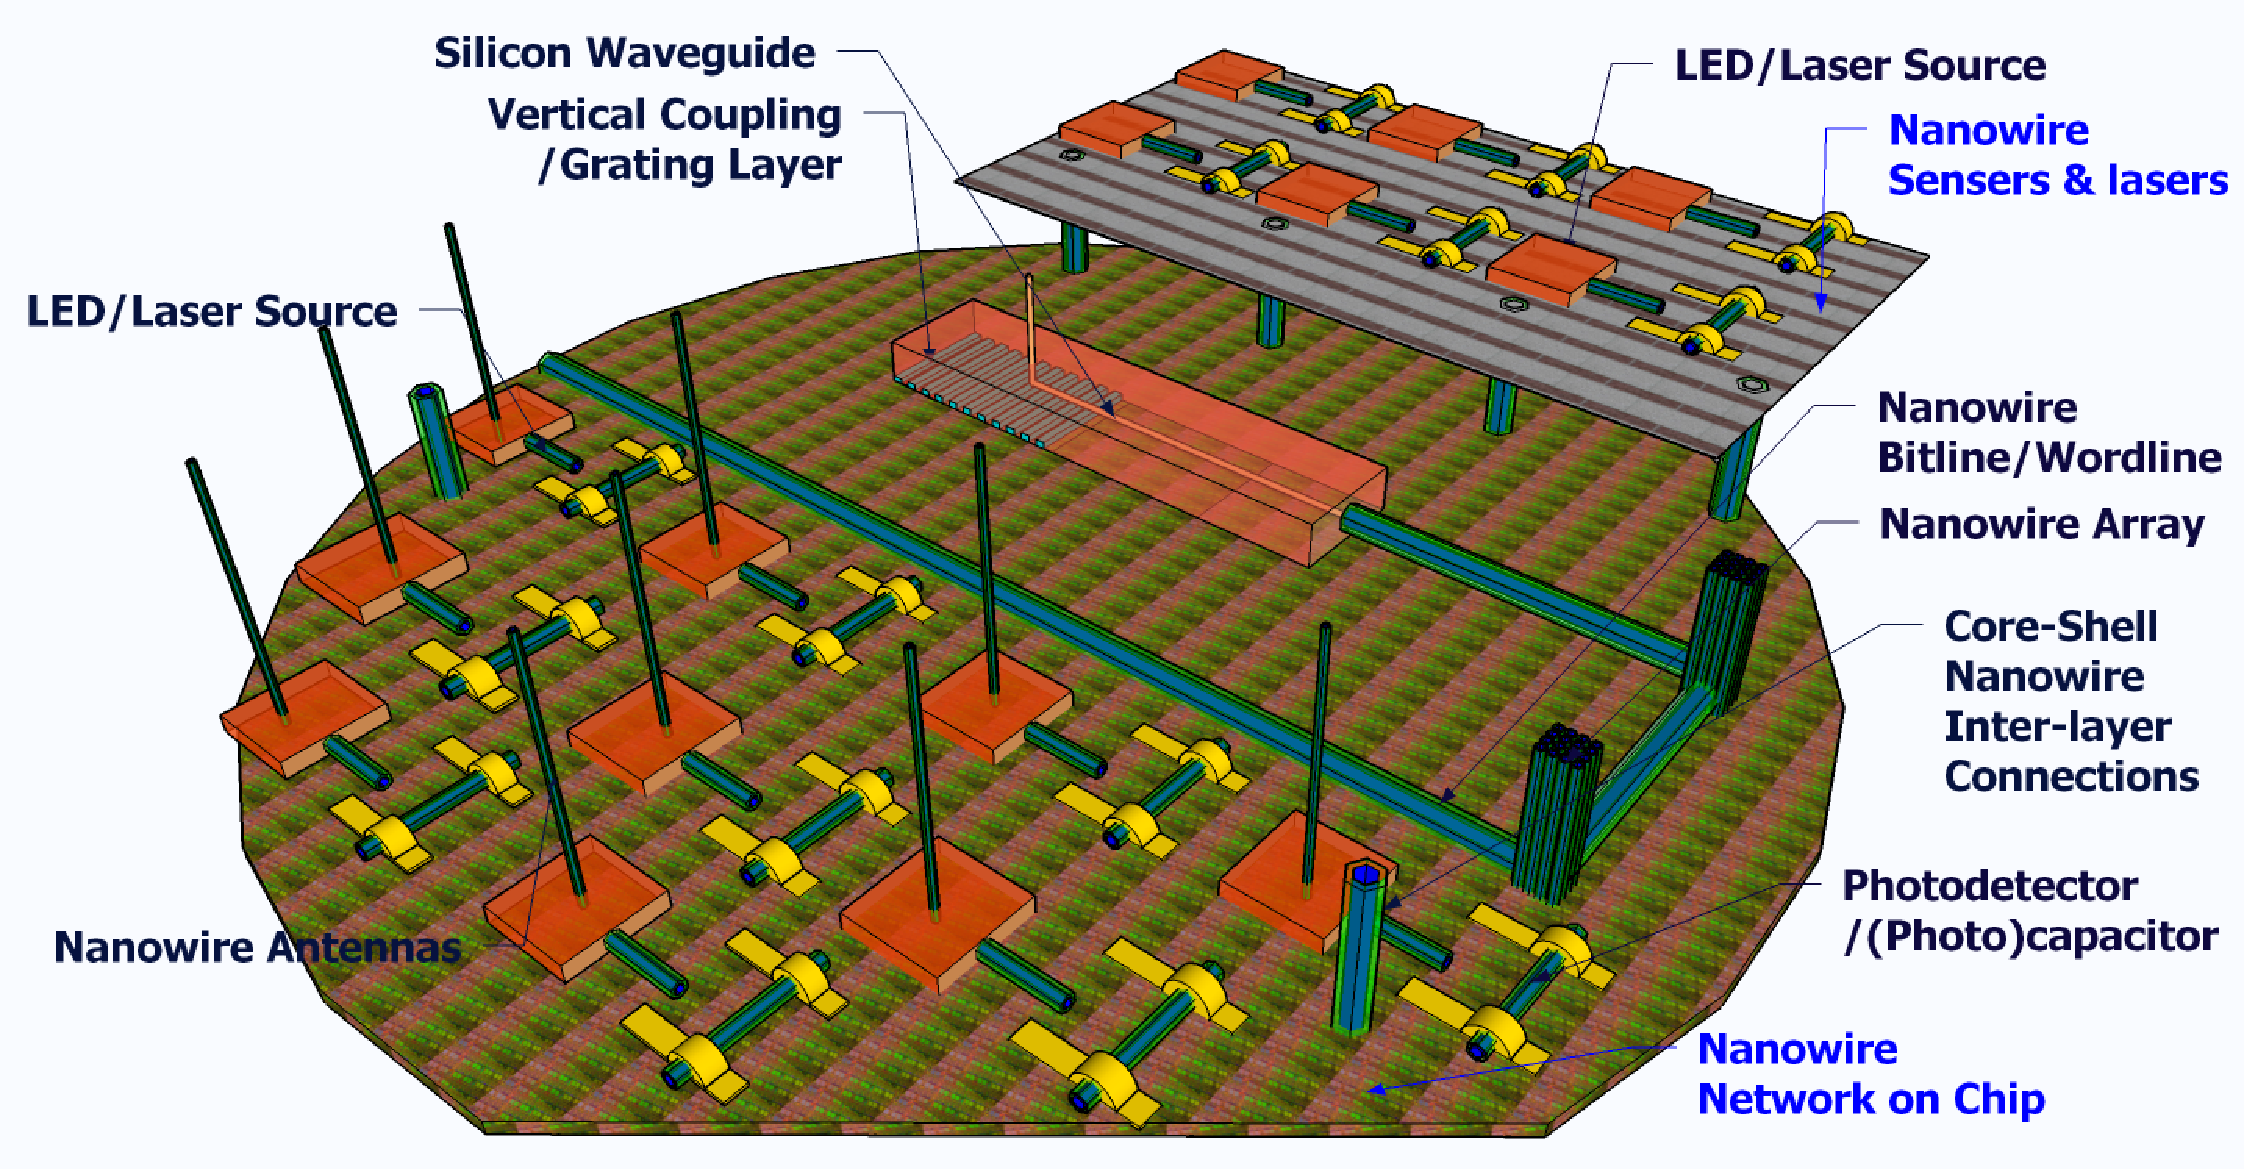
\includegraphics[width=\textwidth]{pictures/Conclusion/NWPIC_NB}
  \label{NWPIC_NB}
\end{figure}
%In Chapter~\ref{data} we brought together data from the mid-IR through the UV
%for the purpose of creating multi-wavelength SEDs for the SDSS DR7 quasars
%catalog.  This involved cross-matching mid-IR data from {\em Spitzer} and {\em
%WISE}, near-IR data from 2MASS and UKIDSS, and UV data from {\em GALEX}.  From
%this cross matched data set we created several subsets used throughout our
%studies.  We began with a (observationally) non-reddened data set used to
%explore trends in the SEDs based on various observed properties. To study the
%dust reddening properties of our quasars we limited our data to quasars
%uniformly selected by the SDSS quasar detection pipeline.  This data set was
%further split into quasar with BALs and quasars without BALs.  Finally, when
%exploring our SEDs as function of $\mbh$ we further limited this sample to the
%non-BAL quasars since BALs can make the estimated values for $\mbh$ invalid.


  
  
\end{thesis}

\suppressfooter{}
\bibliography{bib/All_refs}
\suppressfooter{}
\restorefooter{}
\appendix{}
\chapter{Transition Rates} \label{ch:rates} 

This research project focuses on the dimensional dependence of the absorption
behavior in semiconductor when interacting with light. Through time-dependent
perturbation theory, we find out the transition rate and Fermi’s Golden Rule,
then based on the light interaction Hamiltonian, time average Poynting vector
and matrix element, derive the absorption coefficient for bulk semiconductor
(3-dimension), quantum well (2-dimension) and quantum wire (1-dimension)
structure.  Finally, this report will discuss the partial confinement on the
electron in the conduction band without the hole confined in the valence band
situation.

The Schr{\"o}dinger equation:
\begin{equation}
  \HAM\Psi(r,t) = - \frac{\hbar}{i}\frac{\partial}{\partial t}\Psi(r,t)
\end{equation}

The Hamiltonian $\HAM$ can be expressed as:
\begin{equation}
  \HAM = \HAM_0 + \HAM^\prime(r,t)
\end{equation}

where $\HAM_0$ is the unperturbed part Hamiltonian and is time-independent,
$\HAM^\prime(r,t)$ is the small perturbation.

The solution to the unperturbed part is assumed known:

\begin{eqnarray}
\begin{aligned}
  & \HAM_0\Psi_n(r,t) = - \frac{\hbar}{i}\frac{\partial }{\partial t}\Psi_n(r,t),
  \\
  & \frac{dN_p}{dt} = {\Gamma}v_g{g}N_p + \Gamma\beta_{sp}R_{sp} - \frac{N_p}{\tau_p},
\end{aligned}
\label{eq:unperturbHAM}
\end{eqnarray}

The time-dependent perturbation is assumed to have the form

\begin{equation}
  \HAM = \begin{cases}
    \HAM^\prime(r)e^{-i\omega t} + \HAM^{\prime+}(r)e^{+\omega t}, & t \geq 0 \\
    0, & t < 0
  \end{cases}
\end{equation}

Expand the wave function in terms of the unperturbed solution, we find out $\Psi(r,t)$:

\begin{equation}
  \Psi(r,t) = \sum_{n}a_n(t)\Phi_n(r)e^{(-iE_{n}t/\hbar)}
\end{equation}

$|a_n(t)|^2$ gives the probability that the electron is in the state n at time t.

Substituting the expansion for $\Psi$ into Schr{\"o}dinger equation and using~\ref{eq:unperturbHAM}, we have

\begin{equation}
  \sum_n \frac{da_n(t)}{dt}\Psi_n(r)e^{-iE_{n}t/\hbar} = -\frac{\hbar}{i}\sum_n \HAM^{\prime}(r,t)a_n(t)\Phi_n(r)e^{(-iE_{n}t/\hbar)}
\end{equation}

Taking the inner product with the wave function ${\Phi_m}^\star(r)$, and using
the orthonormal property,

\begin{equation}
  \int{d^3}\bm{r}{{\Phi^\ast}_m}(\bm{r})\Phi_n(\bm{r}) = \delta_{mn}
\end{equation}

We find:

\begin{equation}
\frac{d{a_n(t)}}{dt}=-\frac{i}{\hbar}\sum_{n}a_n(t){\HAM^\prime}_{mn}(t)e^{i\omega_{mn}t}
\end{equation}

where


\begin{eqnarray}
\begin{aligned}
  & {\HAM^\prime}_{mn}(t)=\langle{m}|\HAM^\prime(\bm{r},t)|{n}\rangle \\
  & = \int{\Phi^\ast}_m(\bm{r}){\HAM^\prime}(\bm{r},t)\Psi_n(\bm{r})d^3\bm{r} \\
  & = {\HAM^\prime}_{mn}e^{-i\omega{t}} + {\HAM^\prime}_{mn}e^{+i\omega{t}}
\end{aligned}
\label{eq:HAMintigral}
\end{eqnarray}

\begin{equation}
  {\omega_{mn}}=(E_m-E_n)/\hbar
\end{equation}

and the matrix element is:

\begin{equation}
  {\HAM^\prime}_{mn}(t)=\int{{\Phi^\ast}_m}(\bm{r})\HAM^\prime(\bm{r},t)\Psi_{n}(\bm{r})d^3\bm{r}
\end{equation}

Introducing the perturbation parameter $\lambda$


\begin{equation}
  \HAM=\HAM_0+\lambda\HAM^\prime(\bm{r},t)
\end{equation}

and letting

\begin{equation}
  a_n(t)={a^{(0)}}_n+\lambda{a^{(1)}}_n(t)+\lambda^2{a^{(2)}}_n(t)+\cdots
\end{equation}

we can take the derivative and set $\lambda=1$


\begin{eqnarray}
\begin{aligned}
  & \frac{d{{a^{(0)}}_n(t)}}{dt}=0 \\
  & \frac{d{{a^{(1)}}_n(t)}}{dt}=-\frac{i}{\hbar}\sum_{n}{a^{(0)}_n(t)}{\HAM^\prime}_{mn}(t)e^{i\omega_{mn}t}
\\
  & \frac{d{{a^{(2)}}_n(t)}}{dt}=- \frac{i}{\hbar}\sum_{n}{a^{(1)}_n(t)}{\HAM^\prime}_{mn}(t)e^{i\omega_{mn}t}
\\
\label{eq:probility}
\end{aligned}
\end{eqnarray}

Thus, the zeroth-order solutions for equation~\ref{eq:probility} are constant. Let the electron be at the state i initially

\begin{equation}
  {a^{(0)}}_i(t=0)=1; \quad {a^{(0)}}_m(t)=0, \quad m\neq {i}
\end{equation}

We have the zeroth-order solution

\begin{equation}
  {a^{(0)}}_i(t=0)=1; \quad {a^{(0)}}_m(t)=0, \quad m\neq {i}
\end{equation}

Therefore, the electron stays at the state i in the absence of any perturbation. The first order solution is

\begin{eqnarray}
\begin{aligned}
  & \frac{d{a^{(1)}_n}}{dt}=-\frac{i}{\hbar}{\HAM^\prime}_{mn}(t)e^{i\omega_{mn}t} \\
  & = -\frac{i}{\hbar}[{\HAM^\prime}_{mi}e^{-i(\omega_{mi}-\omega)t}+{\HAM^\prime}_{mi}e^{+i(\omega_{mi}-\omega)t}]
\end{aligned}
\end{eqnarray}

If for final state $m=f$; then integrate above equation, we have

\begin{equation}
{a^{(1)}_{f}(t)}=-\frac{i}{\hbar}[{\HAM^\prime}_{fi}\frac{e^{-i(\omega_{mi}-\omega)t}}{\omega_{fi}-\omega}+{\HAM^{\prime+}}_{fi}\frac{e^{+i(\omega_{mi}-\omega)t}}{\omega_{fi}+\omega}]
\end{equation}

If we consider the photon energy to be near resonance, either $\omega\sim\omega_{fi}$ or $\omega\sim-\omega{fi}$, we find the dominant terms:

\begin{equation}
  {a^{(1)}_{f}(t)}=\frac{4{|{\HAM^\prime}_{fi}|}^2}{\hbar^2}\frac{{sin}^2\frac{t}{2}(\omega_{fi}-\omega)}{{(\omega_{fi}-\omega)}^2} +\frac{4{|{\HAM^\prime}_{fi}|}^2}{\hbar^2}\frac{{sin}^2\frac{t}{2}(\omega_{fi}+\omega)}{{(\omega_{fi}+\omega)}^2}
\end{equation}

where the cross-term has been dropped because it is small compared with either of the above two terms.

When the interaction time is long enough, using approcimation
\begin{equation}
  \frac{{sin}^2(\frac{xt}{2})}{x^2}\rightarrow \frac{\pi{t}}{2}\delta(x)
\end{equation}

Then

\begin{equation}
  {|a^{(1)}_f(t)|}^2= \frac{2\pi{t}}{\hbar^2}{|\HAM^\prime_(fi)|}^2\delta(\omega_{fi}-\omega)+\frac{2\pi{t}}{\hbar^2}{|\HAM^\prime_(fi)|}^2\delta(\omega_{fi}+\omega)
\end{equation}

The transition rate should be, after using the property of

\begin{equation}
  \delta(\hbar\omega)=\frac{\delta(w)}{\hbar}
\end{equation}

\begin{eqnarray}
\begin{aligned}
  & W_{if} = \frac{d{|a^{(1)}_f(t)|}^2}{dt} \\ 
  &  \frac{2\pi}{\hbar}{|\HAM^\prime_(fi)|}^2\delta(E_{f}-E_{i}-\hbar\omega)+\frac{2\pi}{\hbar}{|\HAM^\prime_(fi)|}^2\delta(E_{f}-E_{i}+\hbar\omega)
\end{aligned}
\end{eqnarray}

where $E_f = E_i+ \hbar\omega$ represents the absorption of a photon by an electron, and $E_f = E_i - \hbar\omega$ corresponds with the emission of a photon.

\begin{equation}
  {I_{hm}^{en}}=\int_{-\infty}^\infty{\Phi_n^\ast}(z){g_m(z)}\,\mathrm{d}z,
\end{equation}

\begin{equation}
{I_{hm}^{en}}=\int_{-\infty}^\infty{\Phi_n^\ast}(z){g_m(z)}\,\mathrm{d}z,
\label{eq:seven}
\end{equation}

Therefore, the electron stays at the state i in the absence of any
perturbation. The first order solution is 

If we consider the photon energy to be near resonance, either  or, we find the
dominant terms: The absorption coefficient is a strong function of
dimensionality. The confining situation of the quantum structure will
considerably affect the energy levels, the overlap function of the conduction
and valance band envelope function and also the joint optical density of state.
Through the derivation of the absorption coefficient, we can observe the
interaction between the light and semiconductor.  The next questions should
address: 1. The simulation data for single nanowire abs

\chapter{Semiconductor Laser Modeling}
\label{sec:model}

In this section, we are trying to delve into the mechanics of how an injected
current actually results in an optical output in a semiconductor heterojunction
laser by providing a systematic derivation of the dc light-current
characteristics. First, the rate equation for photon generation and loss in a
laser cavity is developed. This shows that only a small portion of the
spontaneously generated light contributes to the lasing mode. Most of it comes
from the stimulated recombination of carriers. All of the carriers that are
stimulated to recombine by light in a certain mode contribute more photons to
that same mode. Thus, the stimulated carrier recombination/photon generation
process is a gain process. We find the threshold gain for lasing which is the
gain necessary to compensate for cavity losses. The threshold current is the
current required to reach this gain 

For electrons and holes in the active region of a diode laser, only a fraction,
$\eta_i$, of injected current will contribute to the generation of carriers.We
assumed the active regions that are undoped or lightly doped, so that under
high injection levels, charge neutrality applies and the electron density
equals the hole density (i.e., $N = P$ in the active region). Thus, we can
greatly simplify our analysis by specifically tracking only the electron
density, N.

We start with the governing equations of carrier density and photon density in
the active region which is governed by a dynamic process.

\begin{eqnarray}
\begin{aligned}
  & \frac{dN}{dt} = \frac{\eta_{i}I}{qV} - \frac{N}{\tau} - R_{st},
  \\
  & \frac{dN_p}{dt} = {\Gamma}v_g{g}N_p + \Gamma\beta_{sp}R_{sp} - \frac{N_p}{\tau_p},
\end{aligned}
\label{eq:eight}
\end{eqnarray}

where $\beta_{sp}$ is the spontaneous emission factor, defined as the
percentage of the total spontaneous emission coupled into the lasing mode. And it is
just the reciprocal of the number of available optical modes in the bandwidth of
the spontaneous emission for uniform coupling to all modes. The g is Incremental gain
per unit length.

The first term of equation 1 is the rate of injected electrons $G_{gen} =
{\Gamma_{i}I}/{qV}$, ${\Gamma_{i}I}/{q}$ is the number of electrons per
second being injected into the active region, where V is the volume of the
active region. The rest terms are the rate of recombining of electrons per unit
volume in the active region. There are several mechanisms should be considered,
including a spontaneous recombination rate, $R_{sp}$, a nonradiative
recombination rate, $R_{nr}$, a carrier leakage rate, $R_l$ and a net
stimulated recombination, $R_{st}$, including both stimulated absorption and
emission. Which looks like:

\begin{equation}
  R_{rec} = R_{sp} + R_{nr} + R_{l} + R_{st}
\end{equation}

The first three terms on the right refer to the natural or unstimulated carrier
decay processes. The fourth one, $R_{st}$, require the presence of photon.

The natural decay process can be described by a carrier lifetime, $\tau$. In
the absence of photon or a generation term, the rate equation for carrier decay
is $dN/dt = -N/\tau$, where $N/\tau = R_{sp} + R_{nr} + R_{l}$.

The natural decay rate can also be expressed in a power series of the carrier
density, N. We can also rewrite $R_{rec} = BN^2 + (AN + CN^3) + R_{st}$.  Where
$R_{sp} ~ BN^2$ and $R_{nr} + R_{l} ~ (AN + cN^3)$. The coefficient B is the
bimolecular recombination coefficient, and it has a magnitude, $B \sim 10^{-10}
cm^3/s$ for most AlGaAs and InGaAsP alloys of interest.

When a laser is below threshold, in which the gain is insufficient to
compensate for cavity losses, the generated photons do not receive net
amplification. The spontaneous photon generation rate per unit volume is
exactly equal to the spontaneous electron recombination rate, $R_{sp}$, because
an electron-hole pair will emit a photon when they recombine radiatively.
Under steady-state conditions ($dN/dt = 0$), the generation rate equals the
recombination rate with $R_{st} = 0$.

\begin{equation}
  \frac{\eta_{i}I}{qV} = R_{sp} + R_{nr} + R_{l}
\end{equation}

The spontaneously generated optical power, $P_{sp}$, is obtained by multiplying
the number of photons generated per unit time per unit volume, $R_{sp}$, by the
energy per photon, $hv$, and the volume of the active region, V.

\begin{equation}
  P_{sp} = h{\upsilon}VR_{sp} = \eta_i\eta_r\frac{h\upsilon}{q}I
\end{equation}

The main photon generation term above threshold is $R_{st}$. Electron-hole pair
is stimulated to recombine, another photon is generated. But since the cavity
volume occupied by photons, $V_p$, is usually larger than the active region
volume occupied by electrons, V, the photon density generation rate will be
$[V/V_p]R_{st}$, not just $R_{st}$. The electron-photon overlap factor,
$[V/V_p]$, is generally referred to as the confinement factor, $\Gamma$.

\section{Threshold or Steady-State Gain in Lasers} \label{sec:conditionals}

The cavity loss can be characterized by a photon decay constant or lifetime,
$\tau_p$, and the gain necessary to overcome losses, and thus reach threshold.
By assuming steady-state conditions (\ie $dN_p/dt = 0$), and solving for this
steady-state or threshold gain, $g_{th}$, where the generation term equals the
recombination term for photons. We assume only a small fraction of the
spontaneous emission is coupled into the mode (\ie $\beta_{sp}$ is quite
small), then the second term can be neglected, and we have the solution:

\begin{equation}
  \Gamma{g_{th}} = \frac{1}{v_g\tau_p} = <\alpha_i> + \alpha_m
\end{equation}

The product, $\Gamma{g_{th}}$, is referred to as the threshold modal gain
because it now represents the net gain required for the mode as a whole, and it
is the mode as a whole that experiences the cavity loss. $<\alpha_i>$ is the
average internal loss, and $\alpha_m$ is the mirror loss if we considered an
in-plane wave laser.

The optical energy of a nano-cavity laser propagates in a dielectric waveguide
mode, which is confined both transversely and laterally as defined by a
normalized transverse electric field profile, $U(x,y)$. In the axial direction
this mode propagates as $exp^{(-j\beta z)}$, where $\beta$ is the complex
propagation constant, which includes any loss or gain. Thus, the time- and
space-varying electric field can be written as

\begin{equation}
  \xi = \hat{e}_{y}E_{0}U(x,y)e^{j(\omega t- \beta z)}
\end{equation}

where $\hat{e}_y$ is the unit vector indicating TE polarization and $E_0$ is
the magnitude of the field. The complex propagation constant, $\beta$, includes
the incremental transverse modal gain, $<g>_{xy}$ and internal modal loss,
$<\alpha_i>_{xy}$. If we consider a Fabry-Perot laser with the propagating mode
is reflected by end mirrors, and the reflection coefficients are $r_1$ and
$r_2$. respectively. In addition, the mean mirror intensity reflection coefficient, $R = r_1r_2$.

Define the mirror lass as $\alpha_m$

\begin{equation}
  \alpha_m \equiv \frac{1}{L}\ln(\frac{1}{R})
\end{equation}

The photon decay lifetime is given by,

\begin{equation}
  \frac{1}{\tau_p} = \frac{1}{\tau_i} + \frac{1}{\tau_m} = v_g(<\alpha_i> + \alpha_m)
\end{equation}

Thus, we can also write

\begin{equation}
  \Gamma g_{th} = <\alpha_i> + \alpha_m = \frac{1}{v_g\tau_p}
\end{equation}

\section{Threshold Current and Output Power}
\label{sec:threshold_current_and_power_out_versus_current}

We construct together a below-threshold and an above-threshold characteristic
to illustrate the output power versus input current for a normal diode laser.
The first step is to use the below-threshold steady-state carrier rate
equation,

\begin{equation}
  \frac{\eta_{i}I_{th}}{qV} = {(R_{sp} + R_{nr} + R_{l})}_{th} = \frac{N_{th}}{\tau} 
\end{equation}

Then, recognizing that $(R_{sp} + R_{nr} + R_{l}) =AN + BN^2 +CN^3$ depends
monotonically on $N$, we observe from eq 2.34 that above threshold $(R_{sp} +
R_{nr} + R_{l})$ will also clamp at its threshold value, given by Eq 2.35. Thus,
we can substitute Eq 2.35 into the carrier rate equation, eq 2.16 to obtain a
new above threshold carrier rate equations,

\begin{equation}
  \frac{dN}{dt} = \eta_i \frac{(I - I_{th})}{qV} - v_{g}gN_p,~~~   (I > I_{th})
\end{equation}

We also calculate a steady-state photon density above threshold where $g = g_{th}$,

\begin{equation}
  N_p = \frac{\eta_i (I - I_{th})}{qv_{g}g{th}V}~~~   (steady~ state)
\end{equation}

To obtain the power out, we first construct the stored optical energy in the
cavity, $E_{os}$, by multiplying the photon density, $N_p$, by the energy per
photon, $hv$, and the cavity volume, $V_p$. That is $E_{os} = N_phvV_p$. Then,
we multiply this by the erngy loss rate through the mirrors, $v_g\alpha_m =
\frac{1}{\tau_m}$, to get the optical power output from the mirrors,

\begin{equation}
  P_0 = v_g\alpha_{m}N_phvV_p
\end{equation}

Substituting from , and using $\Gamma = V/V_p$,

\begin{equation}
  P_0 = \eta_i(\frac{\alpha_m}{<\alpha_i> + \alpha_m})\frac{hv}{q}(I - I{th}),~~~(I > I_{th})
\end{equation}

For the output power below-threshold $(I < I_{th})$ can be approximated by neglecting the stimulated emission term and solving for $N_p$ under steady-state conditions.

\begin{equation}
N_p = \Gamma\beta_{sp}R_{sp}\tau{p}~~~(I < I_{th})
\end{equation}

and 

\begin{equation}
  P_0(I < I_{th}) = \eta_r\eta_i\left(\frac{\alpha_m}{<\alpha_i> + \alpha_m}\right)\frac{hv}{q}\beta_{sp}I,
\end{equation}


We can get the threshold carrier density

\begin{equation}
  N_{th} = N_{tr}e^{g_{th}/g_{0}N} = N_{tr}e^{(<\alpha_i> + \alpha_m)/\Gamma{g_{0}}N}
\end{equation}

Using the polynomial fit for the recombination rates, and recognizing that for
the best laser material the recombination at threshold is dominated by
spontaneous recombination, we have, $I_{th}\cong B{N_{th}}^2qV/\eta_i$, Thus

\begin{equation}
  I_{th} {\cong} \frac{qVB{N_{tr}}^2}{\eta_i}e^{(<\alpha_i> + \alpha_m)/\Gamma{g_0}N}
\end{equation}

where for most $\uppercase\expandafter{\romannumeral3} -
\uppercase\expandafter{\romannumeral5}$ materials the bimolecular recombination
coefficient, $B \sim 10^{-10} cm^3/s$.

For a multiple quantum-well (MQW) lasers, we have to multiply the single-well confinement factor, $\Gamma_1$, and volume, $V_1$, by the number of wells, $N_w$.


\begin{equation}
  I_{thMQW} {\cong} \frac{qN_{w}V_{1}B{N_{tr}}^2}{\eta_i}e^{2(<\alpha_i> + \alpha_m)/{N_w\Gamma_{1}g_{0}N}}
\end{equation}


\chapter{MEEP Simulation Code} \label{ch:meepcode} 
\section{Cylindrical Core-Shell Nanowire}

%\SyntaxHighLighting{}
\lstinputlisting[language=Scheme]{snippet/sourcecode/CylindCS.ctl}

\section{Hexagonal Core-Shell Nanowire}
%\SyntaxHighLighting{}
\lstinputlisting[language=Scheme]{snippet/sourcecode/HexCS3D.ctl}

\chapter{Gain Spectrum and Threshold Calculation Matlab Code} \label{ch:matlabcode} 
%\SyntaxHighLighting{}
\lstinputlisting[language=matlab]{snippet/sourcecode/gain1band.m}

\suppressfooter{}
\iffinal{}{\newpage}

\begin{vita}

{\Large\bf Coleman M. Krawczyk}

\singlespacing
{\large\bf Education}
\begin{itemize} \itemsep -2pt
\item Drexel University, Philadelphia, Pennsylvania USA
	\vspace{-2pt}
	\begin{itemize} \itemsep -2pt
		\item Ph.D., Physics, September 2014
		\item M.S., Physics, June 2010
	\end{itemize}
	\vspace{-2pt}
\item University of Massachusetts at Amherst, Amherst, Massachusetts USA
	\vspace{-2pt}
	\begin{itemize} \itemsep -2pt
		\item B.S., Astrophysics, May 2008
		\item B.S., Mathematics, May 2008
	\end{itemize}
\end{itemize}

{\large\bf Publications}
\begin{itemize} \itemsep -2pt
	\item ``Dusty Quasars", 2014
	\item ``Mean Spectral Energy Distributions and Bolometric Corrections for Luminous Quasars", \href{http://dx.doi.org/10.1088/0067-0049/206/1/4}{ApJS, 206, 4}, 2013
	\item  ``C IV Emission and the Ultraviolet through X-Ray Spectral Energy Distribution of Radio-quiet Quasars", \href{http://dx.doi.org/10.1088/0004-6256/142/4/130}{AJ, 142, 130}, 2011
	\item  ``The Sloan Digital Sky Survey Quasar Catalog. V. Seventh Data Release", \href{http://dx.doi.org/10.1088/0004-6256/139/6/2360}{AJ, 139, 2360}, 2010
	\item ``Re-Examining Larson's Scaling Relationships in Galactic Molecular Clouds", \href{http://dx.doi.org/10.1088/0004-637X/699/2/1092}{ApJ, 699, 1092}, 2008
\end{itemize}

%{\large\bf Talks}
%\begin{itemize} \itemsep -2pt
%	\item ``Exploring Quasar SEDs as a Function of Black Hole Properties", American Astronomical Society Meeting 223, January 2014
%	\item ``Mean SEDs, Bolometric Corrections, and Dust Reddening for Luminous Quasars", Max Planck Institut f\"{u}r Astronomie, May 2013
%\end{itemize}

{\large\bf Awards}
\begin{itemize} \itemsep -2pt
	\item NSF Graduate Research Fellowship Program, Honorable Mention, 2009
	\item Mary Dailey Irvine Prize, 2008
\end{itemize}

{\large\bf Teaching Experience}

\begin{itemize} \itemsep -2pt
	\item \textbf{Teaching Assistant} \hfill \textit{September 2008 to May 2010}
	\begin{itemize} \itemsep -2pt
		\item[] \textit{Autumn 2008 to Spring 2009} -- Introductory Physics I--III
		\item[]\textit{Autumn 2009 to Spring 2010} -- Contemporary Physics I--III
	\end{itemize}
	\item \textbf{Tutor}%
	\begin{itemize} \itemsep -2pt
		\item[]\textit{Spring 2006 to Spring 2008} -- Astronomy Help Desk
	\end{itemize}
	\item \textbf{Supplemental Instructor} \hfill \textit{Spring 2007  to Spring 2008}
	\begin{itemize} \itemsep -2pt
		\item[]\textit{Spring 2007 and 2008} -- SI for Techniques of Theoretical Physics
		\item[]\textit{Autumn 2008} -- SI for  Mechanics
	\end{itemize}
\end{itemize}

{\large\bf Public Outreach}
\begin{itemize} \itemsep -2pt
	\item \textbf{The Franklin Institute} \hfill \textit{January 2009 to July 2014}
	\item \textbf{Carver Science Fair} \hfill \textit{February 19th, 2014}
	\item \textbf{UMass Science Outreach} \hfill \textit{September 2004 to May 2008}
\end{itemize}

\end{vita}

\restorefooter{}
\end{document}
